\documentclass[twoside]{book}

% Packages required by doxygen
\usepackage{calc}
\usepackage{doxygen}
\usepackage{graphicx}
\usepackage[utf8]{inputenc}
\usepackage{makeidx}
\usepackage{multicol}
\usepackage{multirow}
\usepackage{textcomp}
\usepackage[table]{xcolor}

% Font selection
\usepackage[T1]{fontenc}
\usepackage{mathptmx}
\usepackage[scaled=.90]{helvet}
\usepackage{courier}
\usepackage{amssymb}
\usepackage{sectsty}
\renewcommand{\familydefault}{\sfdefault}
\allsectionsfont{%
  \fontseries{bc}\selectfont%
  \color{darkgray}%
}
\renewcommand{\DoxyLabelFont}{%
  \fontseries{bc}\selectfont%
  \color{darkgray}%
}

% Page & text layout
\usepackage{geometry}
\geometry{%
  a4paper,%
  top=2.5cm,%
  bottom=2.5cm,%
  left=2.5cm,%
  right=2.5cm%
}
\tolerance=750
\hfuzz=15pt
\hbadness=750
\setlength{\emergencystretch}{15pt}
\setlength{\parindent}{0cm}
\setlength{\parskip}{0.2cm}
\makeatletter
\renewcommand{\paragraph}{%
  \@startsection{paragraph}{4}{0ex}{-1.0ex}{1.0ex}{%
    \normalfont\normalsize\bfseries\SS@parafont%
  }%
}
\renewcommand{\subparagraph}{%
  \@startsection{subparagraph}{5}{0ex}{-1.0ex}{1.0ex}{%
    \normalfont\normalsize\bfseries\SS@subparafont%
  }%
}
\makeatother

% Headers & footers
\usepackage{fancyhdr}
\pagestyle{fancyplain}
\fancyhead[LE]{\fancyplain{}{\bfseries\thepage}}
\fancyhead[CE]{\fancyplain{}{}}
\fancyhead[RE]{\fancyplain{}{\bfseries\leftmark}}
\fancyhead[LO]{\fancyplain{}{\bfseries\rightmark}}
\fancyhead[CO]{\fancyplain{}{}}
\fancyhead[RO]{\fancyplain{}{\bfseries\thepage}}
\fancyfoot[LE]{\fancyplain{}{}}
\fancyfoot[CE]{\fancyplain{}{}}
\fancyfoot[RE]{\fancyplain{}{\bfseries\scriptsize Generated on Sat Jan 30 2016 17\-:33\-:27 for Embedded Tool Kit by Doxygen }}
\fancyfoot[LO]{\fancyplain{}{\bfseries\scriptsize Generated on Sat Jan 30 2016 17\-:33\-:27 for Embedded Tool Kit by Doxygen }}
\fancyfoot[CO]{\fancyplain{}{}}
\fancyfoot[RO]{\fancyplain{}{}}
\renewcommand{\footrulewidth}{0.4pt}
\renewcommand{\chaptermark}[1]{%
  \markboth{#1}{}%
}
\renewcommand{\sectionmark}[1]{%
  \markright{\thesection\ #1}%
}

% Indices & bibliography
\usepackage{natbib}
\usepackage[titles]{tocloft}
\setcounter{tocdepth}{3}
\setcounter{secnumdepth}{5}
\makeindex

% Hyperlinks (required, but should be loaded last)
\usepackage{ifpdf}
\ifpdf
  \usepackage[pdftex,pagebackref=true]{hyperref}
\else
  \usepackage[ps2pdf,pagebackref=true]{hyperref}
\fi
\hypersetup{%
  colorlinks=true,%
  linkcolor=blue,%
  citecolor=blue,%
  unicode%
}

% Custom commands
\newcommand{\clearemptydoublepage}{%
  \newpage{\pagestyle{empty}\cleardoublepage}%
}


%===== C O N T E N T S =====

\begin{document}

% Titlepage & ToC
\hypersetup{pageanchor=false}
\pagenumbering{roman}
\begin{titlepage}
\vspace*{7cm}
\begin{center}%
{\Large Embedded Tool Kit }\\
\vspace*{1cm}
{\large Generated by Doxygen 1.8.6}\\
\vspace*{0.5cm}
{\small Sat Jan 30 2016 17:33:27}\\
\end{center}
\end{titlepage}
\clearemptydoublepage
\tableofcontents
\clearemptydoublepage
\pagenumbering{arabic}
\hypersetup{pageanchor=true}

%--- Begin generated contents ---
\chapter{Embedded Tool Kit}
\label{index}\hypertarget{index}{}\hypertarget{index_intro_sec}{}\section{Introduction}\label{index_intro_sec}
E\-T\-K is a lightweight collection of C++ templates and classes that are particularly useful to embedded software engineers.\hypertarget{index_requirements_sec}{}\section{Requirements}\label{index_requirements_sec}
E\-T\-K uses C++14 language features. This means it requires at least g++-\/4.9 or an equivalent compiler to use.

Robot graphic by \href{http://www.freepik.com/}{\tt Freepik} from \href{http://www.flaticon.com/}{\tt Flaticon} is licensed under \href{http://creativecommons.org/licenses/by/3.0/}{\tt C\-C B\-Y 3.\-0}. Made with \href{http://logomakr.com}{\tt Logo Maker} 
\chapter{Namespace Index}
\section{Namespace List}
Here is a list of all documented namespaces with brief descriptions\-:\begin{DoxyCompactList}
\item\contentsline{section}{\hyperlink{namespaceetk}{etk} }{\pageref{namespaceetk}}{}
\end{DoxyCompactList}

\chapter{Hierarchical Index}
\section{Class Hierarchy}
This inheritance list is sorted roughly, but not completely, alphabetically\-:\begin{DoxyCompactList}
\item \contentsline{section}{etk\-:\-:Array$<$ T, L $>$}{\pageref{classetk_1_1_array}}{}
\item \contentsline{section}{etk\-:\-:Array$<$ etk\-:\-:Evo\-Pid\-:\-:P\-I\-D\-Gain, P\-O\-P\-U\-L\-A\-T\-I\-O\-N $>$}{\pageref{classetk_1_1_array}}{}
\item \contentsline{section}{etk\-:\-:Array$<$ tbl, N $>$}{\pageref{classetk_1_1_array}}{}
\item \contentsline{section}{etk\-:\-:Bits$<$ T $>$}{\pageref{classetk_1_1_bits}}{}
\item \contentsline{section}{etk\-:\-:Brown\-Linear\-Expo}{\pageref{classetk_1_1_brown_linear_expo}}{}
\item \contentsline{section}{etk\-:\-:Coordinate}{\pageref{classetk_1_1_coordinate}}{}
\begin{DoxyCompactList}
\item \contentsline{section}{etk\-:\-:Waypoint}{\pageref{classetk_1_1_waypoint}}{}
\end{DoxyCompactList}
\item \contentsline{section}{etk\-:\-:Evo\-Pid}{\pageref{classetk_1_1_evo_pid}}{}
\item \contentsline{section}{etk\-:\-:Expo\-Moving\-Avg}{\pageref{classetk_1_1_expo_moving_avg}}{}
\item \contentsline{section}{etk\-:\-:Fuzzy$<$ N $>$}{\pageref{classetk_1_1_fuzzy}}{}
\item \contentsline{section}{etk\-:\-:High\-Pass\-Filter}{\pageref{classetk_1_1_high_pass_filter}}{}
\item \contentsline{section}{etk\-:\-:Short\-Term\-Memory$<$ T, L\-E\-N $>$\-:\-:Iterator}{\pageref{classetk_1_1_short_term_memory_1_1_iterator}}{}
\item \contentsline{section}{etk\-:\-:Array$<$ T, L $>$\-:\-:Iterator}{\pageref{classetk_1_1_array_1_1_iterator}}{}
\item \contentsline{section}{etk\-:\-:List$<$ T, L $>$\-:\-:Iterator}{\pageref{classetk_1_1_list_1_1_iterator}}{}
\item \contentsline{section}{etk\-:\-:List$<$ T, L $>$}{\pageref{classetk_1_1_list}}{}
\item \contentsline{section}{etk\-:\-:List$<$ etk\-:\-:Fuzzy\-:\-:Set, N+1 $>$}{\pageref{classetk_1_1_list}}{}
\item \contentsline{section}{etk\-:\-:Loop\-Range$<$ T $>$}{\pageref{classetk_1_1_loop_range}}{}
\item \contentsline{section}{etk\-:\-:Loop\-Range\-Iterator$<$ T $>$}{\pageref{classetk_1_1_loop_range_iterator}}{}
\item \contentsline{section}{etk\-:\-:Matrix$<$ M\-A\-X\-\_\-\-X, M\-A\-X\-\_\-\-Y $>$}{\pageref{classetk_1_1_matrix}}{}
\item \contentsline{section}{etk\-:\-:Obj\-Pool$<$ T, N $>$}{\pageref{classetk_1_1_obj_pool}}{}
\item \contentsline{section}{etk\-:\-:P\-I\-D\-Controller}{\pageref{classetk_1_1_p_i_d_controller}}{}
\begin{DoxyCompactList}
\item \contentsline{section}{etk\-:\-:Circular\-P\-I\-D\-Controller}{\pageref{classetk_1_1_circular_p_i_d_controller}}{}
\end{DoxyCompactList}
\item \contentsline{section}{etk\-:\-:Evo\-Pid\-:\-:P\-I\-D\-Gain}{\pageref{classetk_1_1_evo_pid_1_1_p_i_d_gain}}{}
\item \contentsline{section}{etk\-:\-:P\-I\-D\-Rater}{\pageref{classetk_1_1_p_i_d_rater}}{}
\begin{DoxyCompactList}
\item \contentsline{section}{etk\-:\-:Basic\-P\-I\-D\-Rater}{\pageref{classetk_1_1_basic_p_i_d_rater}}{}
\end{DoxyCompactList}
\item \contentsline{section}{etk\-:\-:Pool\-Ptr$<$ P, T $>$}{\pageref{classetk_1_1_pool_ptr}}{}
\item \contentsline{section}{etk\-:\-:Quaternion}{\pageref{classetk_1_1_quaternion}}{}
\item \contentsline{section}{etk\-:\-:Rate\-Limiter}{\pageref{classetk_1_1_rate_limiter}}{}
\item \contentsline{section}{etk\-:\-:Ring\-Buffer$<$ T, overwrite $>$}{\pageref{classetk_1_1_ring_buffer}}{}
\item \contentsline{section}{etk\-:\-:Rope}{\pageref{classetk_1_1_rope}}{}
\item \contentsline{section}{etk\-:\-:scalar\-Linear\-Kalman}{\pageref{classetk_1_1scalar_linear_kalman}}{}
\item \contentsline{section}{etk\-:\-:Fuzzy$<$ N $>$\-:\-:Set}{\pageref{classetk_1_1_fuzzy_1_1_set}}{}
\item \contentsline{section}{etk\-:\-:Short\-Term\-Memory$<$ T, L\-E\-N $>$}{\pageref{classetk_1_1_short_term_memory}}{}
\item \contentsline{section}{etk\-:\-:Short\-Term\-Memory$<$ real\-\_\-t, M\-E\-M\-O\-R\-Y\-\_\-\-L\-E\-N\-G\-T\-H $>$}{\pageref{classetk_1_1_short_term_memory}}{}
\item \contentsline{section}{etk\-:\-:Static\-String$<$ L $>$}{\pageref{classetk_1_1_static_string}}{}
\item \contentsline{section}{etk\-:\-:Stream$<$ derived $>$}{\pageref{classetk_1_1_stream}}{}
\item \contentsline{section}{etk\-:\-:Time}{\pageref{classetk_1_1_time}}{}
\item \contentsline{section}{etk\-:\-:Tokeniser$<$ T $>$}{\pageref{classetk_1_1_tokeniser}}{}
\item \contentsline{section}{etk\-:\-:Vector$<$ N $>$}{\pageref{classetk_1_1_vector}}{}
\end{DoxyCompactList}

\chapter{Class Index}
\section{Class List}
Here are the classes, structs, unions and interfaces with brief descriptions\-:\begin{DoxyCompactList}
\item\contentsline{section}{\hyperlink{classetk_1_1_array}{etk\-::\-Array$<$ T, L $>$} }{\pageref{classetk_1_1_array}}{}
\item\contentsline{section}{\hyperlink{classetk_1_1_basic_p_i_d_rater}{etk\-::\-Basic\-P\-I\-D\-Rater} }{\pageref{classetk_1_1_basic_p_i_d_rater}}{}
\item\contentsline{section}{\hyperlink{classetk_1_1_bits}{etk\-::\-Bits$<$ T $>$} \\*\hyperlink{classetk_1_1_bits}{Bits} provides an easy way to set and read the bits of an integer individually }{\pageref{classetk_1_1_bits}}{}
\item\contentsline{section}{\hyperlink{classetk_1_1_brown_linear_expo}{etk\-::\-Brown\-Linear\-Expo} \\*Browns linear exponential filter is a form of double exponential smoothing. It can be more responsive than the Moving\-Expo\-Avg filter, but is prone to overshoot }{\pageref{classetk_1_1_brown_linear_expo}}{}
\item\contentsline{section}{\hyperlink{classetk_1_1_circular_p_i_d_controller}{etk\-::\-Circular\-P\-I\-D\-Controller} \\*A Circular P\-I\-D Controller. This controller uses \hyperlink{namespaceetk_a77f395cb44512ab4a95d08b01b3c7f20}{constrain\-\_\-circular()}; to keep it's inputs and error within a circular range. If segments was set to 360, the setpoint was 175 and the measurement was -\/175, the resulting error would be -\/10 degrees. This makes the circular P\-I\-D controller suitable for controlling the heading of a vehicle, for example }{\pageref{classetk_1_1_circular_p_i_d_controller}}{}
\item\contentsline{section}{\hyperlink{classetk_1_1_coordinate}{etk\-::\-Coordinate} \\*Represents latitude and longitude coordinates. Units are in degrees unless stated otherwise. All navigation functions use great circle mathematics and are, in theory, suitable for long distances and navigation in polar regions }{\pageref{classetk_1_1_coordinate}}{}
\item\contentsline{section}{\hyperlink{classetk_1_1_evo_pid}{etk\-::\-Evo\-Pid} \\*A self tuning P\-I\-D controller that uses Evolutionary Algorithms to search for optimal P\-I\-D gains }{\pageref{classetk_1_1_evo_pid}}{}
\item\contentsline{section}{\hyperlink{classetk_1_1_expo_moving_avg}{etk\-::\-Expo\-Moving\-Avg} \\*An exponential moving average low-\/pass filter }{\pageref{classetk_1_1_expo_moving_avg}}{}
\item\contentsline{section}{\hyperlink{classetk_1_1_fuzzy}{etk\-::\-Fuzzy$<$ N $>$} \\*\hyperlink{classetk_1_1_fuzzy}{Fuzzy} logic class. \hyperlink{classetk_1_1_fuzzy}{Fuzzy} logic can be used for function approximation, control applications, signal process, A\-I and so on. Here is a tutorial on using \hyperlink{classetk_1_1_fuzzy}{Fuzzy} logic with E\-T\-K \href{http://www.camelsoftware.com/blog/2015/12/12/fuzzy-logic-control-part-1/}{\tt http\-://www.\-camelsoftware.\-com/blog/2015/12/12/fuzzy-\/logic-\/control-\/part-\/1/} }{\pageref{classetk_1_1_fuzzy}}{}
\item\contentsline{section}{\hyperlink{classetk_1_1_high_pass_filter}{etk\-::\-High\-Pass\-Filter} \\*The \hyperlink{classetk_1_1_high_pass_filter}{High\-Pass\-Filter} blocks long term averages and allows higher frequencies through }{\pageref{classetk_1_1_high_pass_filter}}{}
\item\contentsline{section}{\hyperlink{classetk_1_1_short_term_memory_1_1_iterator}{etk\-::\-Short\-Term\-Memory$<$ T, L\-E\-N $>$\-::\-Iterator} }{\pageref{classetk_1_1_short_term_memory_1_1_iterator}}{}
\item\contentsline{section}{\hyperlink{classetk_1_1_array_1_1_iterator}{etk\-::\-Array$<$ T, L $>$\-::\-Iterator} }{\pageref{classetk_1_1_array_1_1_iterator}}{}
\item\contentsline{section}{\hyperlink{classetk_1_1_list_1_1_iterator}{etk\-::\-List$<$ T, L $>$\-::\-Iterator} \\*The list iterator makes a list iterable using C++11 ranged for loop syntax }{\pageref{classetk_1_1_list_1_1_iterator}}{}
\item\contentsline{section}{\hyperlink{classetk_1_1_list}{etk\-::\-List$<$ T, L $>$} \\*The list class is an iterable container object. A list can contain up to a maximum number of items determined by the template parameter L. \hyperlink{classetk_1_1_list}{List} is supposed to provide a similar look and feel to std\-::vector, but without using dynamic memory allocation }{\pageref{classetk_1_1_list}}{}
\item\contentsline{section}{\hyperlink{classetk_1_1_loop_range}{etk\-::\-Loop\-Range$<$ T $>$} \\*This class is of limited usefullness by itself. It should be used with the \hyperlink{namespaceetk_aff39b0f367ee4d947e2e7d297ffd506b}{range()} template functions }{\pageref{classetk_1_1_loop_range}}{}
\item\contentsline{section}{\hyperlink{classetk_1_1_loop_range_iterator}{etk\-::\-Loop\-Range\-Iterator$<$ T $>$} \\*See \hyperlink{classetk_1_1_loop_range}{Loop\-Range} }{\pageref{classetk_1_1_loop_range_iterator}}{}
\item\contentsline{section}{\hyperlink{classetk_1_1_matrix}{etk\-::\-Matrix$<$ M\-A\-X\-\_\-\-X, M\-A\-X\-\_\-\-Y $>$} }{\pageref{classetk_1_1_matrix}}{}
\item\contentsline{section}{\hyperlink{classetk_1_1_obj_pool}{etk\-::\-Obj\-Pool$<$ T, N $>$} }{\pageref{classetk_1_1_obj_pool}}{}
\item\contentsline{section}{\hyperlink{classetk_1_1_p_i_d_controller}{etk\-::\-P\-I\-D\-Controller} \\*A generic \hyperlink{classetk_1_1_p_i_d_controller}{P\-I\-D\-Controller}. \href{https://en.wikipedia.org/wiki/PID_controller}{\tt https\-://en.\-wikipedia.\-org/wiki/\-P\-I\-D\-\_\-controller} }{\pageref{classetk_1_1_p_i_d_controller}}{}
\item\contentsline{section}{\hyperlink{classetk_1_1_evo_pid_1_1_p_i_d_gain}{etk\-::\-Evo\-Pid\-::\-P\-I\-D\-Gain} }{\pageref{classetk_1_1_evo_pid_1_1_p_i_d_gain}}{}
\item\contentsline{section}{\hyperlink{classetk_1_1_p_i_d_rater}{etk\-::\-P\-I\-D\-Rater} }{\pageref{classetk_1_1_p_i_d_rater}}{}
\item\contentsline{section}{\hyperlink{classetk_1_1_pool_ptr}{etk\-::\-Pool\-Ptr$<$ P, T $>$} }{\pageref{classetk_1_1_pool_ptr}}{}
\item\contentsline{section}{\hyperlink{classetk_1_1_quaternion}{etk\-::\-Quaternion} }{\pageref{classetk_1_1_quaternion}}{}
\item\contentsline{section}{\hyperlink{classetk_1_1_rate_limiter}{etk\-::\-Rate\-Limiter} \\*The \hyperlink{classetk_1_1_rate_limiter}{Rate\-Limiter} limits the rate of change of a signal to a given step size }{\pageref{classetk_1_1_rate_limiter}}{}
\item\contentsline{section}{\hyperlink{classetk_1_1_ring_buffer}{etk\-::\-Ring\-Buffer$<$ T, overwrite $>$} \\*Ring\-Buffers are a great way to buffer information from data streams such as U\-A\-R\-Ts. \hyperlink{classetk_1_1_ring_buffer}{Ring\-Buffer} does not allocate it's own memory, instead it requires a pointer to an array or memory region where it can store data. \par
\par
 Example }{\pageref{classetk_1_1_ring_buffer}}{}
\item\contentsline{section}{\hyperlink{classetk_1_1_rope}{etk\-::\-Rope} \\*W\-H\-Y R\-O\-P\-E? It's like a string, only more robust }{\pageref{classetk_1_1_rope}}{}
\item\contentsline{section}{\hyperlink{classetk_1_1scalar_linear_kalman}{etk\-::scalar\-Linear\-Kalman} \\*A linear kalman filter for scalars }{\pageref{classetk_1_1scalar_linear_kalman}}{}
\item\contentsline{section}{\hyperlink{classetk_1_1_fuzzy_1_1_set}{etk\-::\-Fuzzy$<$ N $>$\-::\-Set} \\*A fuzzy logic set }{\pageref{classetk_1_1_fuzzy_1_1_set}}{}
\item\contentsline{section}{\hyperlink{classetk_1_1_short_term_memory}{etk\-::\-Short\-Term\-Memory$<$ T, L\-E\-N $>$} \\*\hyperlink{classetk_1_1_short_term_memory}{Short\-Term\-Memory} stores a data in a buffer. As more data is received, the old data is eventually overwritten and forgotten. It has some uses in digital signal processing, adaptive control and filtering }{\pageref{classetk_1_1_short_term_memory}}{}
\item\contentsline{section}{\hyperlink{classetk_1_1_static_string}{etk\-::\-Static\-String$<$ L $>$} \\*Static\-Strings are a safer alternative to C-\/strings as Static\-Strings are immune to buf overruns. Static\-Strings also provide a lot of the convenience of std\-::strings, although they do differ from std\-::strings in a number of ways }{\pageref{classetk_1_1_static_string}}{}
\item\contentsline{section}{\hyperlink{classetk_1_1_stream}{etk\-::\-Stream$<$ derived $>$} }{\pageref{classetk_1_1_stream}}{}
\item\contentsline{section}{\hyperlink{classetk_1_1_time}{etk\-::\-Time} \\*\hyperlink{classetk_1_1_time}{Time} is a class that can be used to perform time related functions such as counting systicks }{\pageref{classetk_1_1_time}}{}
\item\contentsline{section}{\hyperlink{classetk_1_1_tokeniser}{etk\-::\-Tokeniser$<$ T $>$} \\*The tokeniser moves along a string and breaks it into tokens }{\pageref{classetk_1_1_tokeniser}}{}
\item\contentsline{section}{\hyperlink{classetk_1_1_vector}{etk\-::\-Vector$<$ N $>$} }{\pageref{classetk_1_1_vector}}{}
\item\contentsline{section}{\hyperlink{classetk_1_1_waypoint}{etk\-::\-Waypoint} \\*A \hyperlink{classetk_1_1_waypoint}{Waypoint} I\-S\-\_\-\-A coordinate, but it has an extra dimension to store altitude. It provides get and set methods for altitude, and it can be cast to a 3 dimensional \hyperlink{classetk_1_1_vector}{etk\-::\-Vector} }{\pageref{classetk_1_1_waypoint}}{}
\end{DoxyCompactList}

\chapter{Namespace Documentation}
\hypertarget{namespaceetk}{\section{etk Namespace Reference}
\label{namespaceetk}\index{etk@{etk}}
}
\subsection*{Namespaces}
\begin{DoxyCompactItemize}
\item 
\hyperlink{namespaceetk_1_1_version}{Version}
\end{DoxyCompactItemize}
\subsection*{Classes}
\begin{DoxyCompactItemize}
\item 
class \hyperlink{classetk_1_1_bits}{Bits}
\begin{DoxyCompactList}\small\item\em \hyperlink{classetk_1_1_bits}{Bits} provides an easy way to set and read the bits of an integer individually. \end{DoxyCompactList}\item 
class \hyperlink{classetk_1_1_cout}{Cout}
\item 
class \hyperlink{classetk_1_1_expo_moving_avg}{Expo\-Moving\-Avg}
\begin{DoxyCompactList}\small\item\em An exponential moving average low-\/pass filter. \end{DoxyCompactList}\item 
class \hyperlink{classetk_1_1_brown_linear_expo}{Brown\-Linear\-Expo}
\begin{DoxyCompactList}\small\item\em Browns linear exponential filter is a form of double exponential smoothing. It can be more responsive than the Moving\-Expo\-Avg filter, but is prone to overshoot. \end{DoxyCompactList}\item 
class \hyperlink{classetk_1_1scalar_linear_kalman}{scalar\-Linear\-Kalman}
\begin{DoxyCompactList}\small\item\em A linear kalman filter for scalars. \end{DoxyCompactList}\item 
class \hyperlink{classetk_1_1_high_pass_filter}{High\-Pass\-Filter}
\begin{DoxyCompactList}\small\item\em The \hyperlink{classetk_1_1_high_pass_filter}{High\-Pass\-Filter} blocks long term averages and allows higher frequencies through. \end{DoxyCompactList}\item 
class \hyperlink{classetk_1_1_rate_limiter}{Rate\-Limiter}
\begin{DoxyCompactList}\small\item\em The \hyperlink{classetk_1_1_rate_limiter}{Rate\-Limiter} limits the rate of change of a signal to a given step size. \end{DoxyCompactList}\item 
class \hyperlink{classetk_1_1_fuzzy}{Fuzzy}
\begin{DoxyCompactList}\small\item\em \hyperlink{classetk_1_1_fuzzy}{Fuzzy} logic class. \hyperlink{classetk_1_1_fuzzy}{Fuzzy} logic can be used for function approximation, control applications, signal process, A\-I and so on. Here is a tutorial on using \hyperlink{classetk_1_1_fuzzy}{Fuzzy} logic with E\-T\-K \href{http://www.camelsoftware.com/blog/2015/12/12/fuzzy-logic-control-part-1/}{\tt http\-://www.\-camelsoftware.\-com/blog/2015/12/12/fuzzy-\/logic-\/control-\/part-\/1/}. \end{DoxyCompactList}\item 
class \hyperlink{classetk_1_1_list}{List}
\begin{DoxyCompactList}\small\item\em The list class is an iterable container object. A list can contain up to a maximum number of items determined by the template parameter L. \hyperlink{classetk_1_1_list}{List} is supposed to provide a similar look and feel to std\-::vector, but without using dynamic memory allocation. \end{DoxyCompactList}\item 
class \hyperlink{classetk_1_1_loop_range_iterator}{Loop\-Range\-Iterator}
\begin{DoxyCompactList}\small\item\em See \hyperlink{classetk_1_1_loop_range}{Loop\-Range}. \end{DoxyCompactList}\item 
class \hyperlink{classetk_1_1_loop_range}{Loop\-Range}
\begin{DoxyCompactList}\small\item\em This class is of limited usefullness by itself. It should be used with the \hyperlink{namespaceetk_aff39b0f367ee4d947e2e7d297ffd506b}{range()} template functions. \end{DoxyCompactList}\item 
class \hyperlink{classetk_1_1_matrix}{Matrix}
\item 
class \hyperlink{classetk_1_1_coordinate}{Coordinate}
\begin{DoxyCompactList}\small\item\em Represents latitude and longitude coordinates. Units are in degrees unless stated otherwise. All navigation functions use great circle mathematics and are, in theory, suitable for long distances and navigation in polar regions. \end{DoxyCompactList}\item 
class \hyperlink{classetk_1_1_waypoint}{Waypoint}
\begin{DoxyCompactList}\small\item\em A \hyperlink{classetk_1_1_waypoint}{Waypoint} I\-S\-\_\-\-A coordinate, but it has an extra dimension to store altitude. It provides get and set methods for altitude, and it can be cast to a 3 dimensional \hyperlink{classetk_1_1_vector}{etk\-::\-Vector}. \end{DoxyCompactList}\item 
class \hyperlink{classetk_1_1_p_i_d_controller}{P\-I\-D\-Controller}
\begin{DoxyCompactList}\small\item\em A generic \hyperlink{classetk_1_1_p_i_d_controller}{P\-I\-D\-Controller}. \href{https://en.wikipedia.org/wiki/PID_controller}{\tt https\-://en.\-wikipedia.\-org/wiki/\-P\-I\-D\-\_\-controller}. \end{DoxyCompactList}\item 
class \hyperlink{classetk_1_1_circular_p_i_d_controller}{Circular\-P\-I\-D\-Controller}
\begin{DoxyCompactList}\small\item\em A Circular P\-I\-D Controller. This controller uses \hyperlink{namespaceetk_a0bb96bed2b97ddb4eba560684c0e050a}{constrain\-\_\-circular()}; to keep it's inputs and error within a circular range. If segments was set to 360, the setpoint was 175 and the measurement was -\/175, the resulting error would be -\/10 degrees. This makes the circular P\-I\-D controller suitable for controlling the heading of a vehicle, for example. \end{DoxyCompactList}\item 
class \hyperlink{classetk_1_1_quaternion}{Quaternion}
\item 
class \hyperlink{classetk_1_1_ring_buffer}{Ring\-Buffer}
\begin{DoxyCompactList}\small\item\em Ring\-Buffers are a great way to buffer information from data streams such as U\-A\-R\-Ts. \hyperlink{classetk_1_1_ring_buffer}{Ring\-Buffer} does not allocate it's own memory, instead it requires a pointer to an array or memory region where it can store data. \par
\par
 Example. \end{DoxyCompactList}\item 
class \hyperlink{classetk_1_1_rope}{Rope}
\begin{DoxyCompactList}\small\item\em W\-H\-Y R\-O\-P\-E? It's like a string, only more robust. \end{DoxyCompactList}\item 
class \hyperlink{classetk_1_1_static_string}{Static\-String}
\begin{DoxyCompactList}\small\item\em Static\-Strings are a safer alternative to C-\/strings as Static\-Strings are immune to buffer overruns. Static\-Strings also provide a lot of the convenience of std\-::strings, although they do differ from std\-::strings in a number of ways. \end{DoxyCompactList}\item 
class \hyperlink{classetk_1_1_short_term_memory}{Short\-Term\-Memory}
\begin{DoxyCompactList}\small\item\em \hyperlink{classetk_1_1_short_term_memory}{Short\-Term\-Memory} stores a data in a buffer. As more data is received, the old data is eventually overwritten and forgotten. It has some uses in digital signal processing, adaptive control and filtering. \end{DoxyCompactList}\item 
class \hyperlink{classetk_1_1_time}{Time}
\begin{DoxyCompactList}\small\item\em \hyperlink{classetk_1_1_time}{Time} is a class that can be used to perform time related functions such as counting systicks. \end{DoxyCompactList}\item 
class \hyperlink{classetk_1_1_tokeniser}{Tokeniser}
\begin{DoxyCompactList}\small\item\em The tokeniser moves along a string and breaks it into tokens. \end{DoxyCompactList}\item 
class \hyperlink{classetk_1_1_vector}{Vector}
\end{DoxyCompactItemize}
\subsection*{Functions}
\begin{DoxyCompactItemize}
\item 
{\footnotesize template$<$typename T $>$ }\\\hyperlink{classetk_1_1_loop_range}{Loop\-Range}$<$ T $>$ \hyperlink{namespaceetk_aff39b0f367ee4d947e2e7d297ffd506b}{range} (T from, T to)
\begin{DoxyCompactList}\small\item\em Like \hyperlink{namespaceetk_a65f1ea4495206c62f285e48ffd2f677e}{range(\-T to)}, except the start value can be specified. \end{DoxyCompactList}\item 
{\footnotesize template$<$typename T $>$ }\\\hyperlink{classetk_1_1_loop_range}{Loop\-Range}$<$ T $>$ \hyperlink{namespaceetk_a65f1ea4495206c62f285e48ffd2f677e}{range} (T to)
\begin{DoxyCompactList}\small\item\em The range function constructs and returns a loop range iterator. It's purpose is to exploit C++11 ranged look syntax and provide a cleaner and less verbose way to iterate over a range of numbers. \end{DoxyCompactList}\item 
auto \hyperlink{namespaceetk_a3b8ba4e0ed638ad07a7ab4f6cfc22c26}{constrain} (auto x, auto a, auto b)
\begin{DoxyCompactList}\small\item\em Used to keep a number within a particular range. \end{DoxyCompactList}\item 
auto \hyperlink{namespaceetk_a0bb96bed2b97ddb4eba560684c0e050a}{constrain\-\_\-circular} (auto x, uint32\-\_\-t segments)
\begin{DoxyCompactList}\small\item\em Used to constrain a number to within a circular range. For example,. \end{DoxyCompactList}\item 
auto \hyperlink{namespaceetk_a6643ab662d2d880d937a8adfea183ac6}{min} (auto a, auto b)
\begin{DoxyCompactList}\small\item\em Returns the smaller of two values. \end{DoxyCompactList}\item 
auto \hyperlink{namespaceetk_a0b90340a93fcebfc57cb7c5f30bed26d}{max} (auto a, auto b)
\begin{DoxyCompactList}\small\item\em Returns the larger of two values. \end{DoxyCompactList}\item 
auto \hyperlink{namespaceetk_a5c4722af8a58319b06077130fe759644}{map} (auto x, auto in\-\_\-min, auto in\-\_\-max, auto out\-\_\-min, auto out\-\_\-max)
\begin{DoxyCompactList}\small\item\em Converts a value from one scale to another. For example, a control functions returns a value between -\/1.\-0 and 1.\-0. The servo requires an input from 0 -\/ 90. ctrl\-\_\-val = map(ctrl\-\_\-val, -\/1.\-0, 1.\-0, 0.\-0, 90.\-0);. \end{DoxyCompactList}\item 
auto \hyperlink{namespaceetk_a29b7cb3d14a2ff168ee94a40797577fe}{copysign} (auto x, auto y)
\begin{DoxyCompactList}\small\item\em Returns a number with the value of x and the sign of y. \end{DoxyCompactList}\item 
auto \hyperlink{namespaceetk_a784f32aa2a3661196e1cf73218c53670}{copysign\-\_\-zero} (auto x, auto y)
\begin{DoxyCompactList}\small\item\em Same as \hyperlink{namespaceetk_a29b7cb3d14a2ff168ee94a40797577fe}{copysign()}, but if y is zero then zero will be returned regardless of x. \end{DoxyCompactList}\item 
void \hyperlink{namespaceetk_ad6c98a88251cf3ccfeabc675507ee871}{swap} (auto \&a, auto \&b)
\begin{DoxyCompactList}\small\item\em Moves a to b and b to a. \end{DoxyCompactList}\item 
bool \hyperlink{namespaceetk_a445cf4f2d0d126c0a1b67891f03408a6}{compare} (auto a, auto b, auto precision)
\begin{DoxyCompactList}\small\item\em Compares two values. Returns true if their difference is less than precision. \end{DoxyCompactList}\item 
{\footnotesize template$<$typename T $>$ }\\void \hyperlink{namespaceetk_abc861c6adcc9b0a83ccca68458756e4d}{bubble\-\_\-sort\-\_\-up} (T $\ast$items, uint32\-\_\-t n)
\begin{DoxyCompactList}\small\item\em Sorts an array using a simple bubble sort algorithm. The largest value will end up at the start of the array. \end{DoxyCompactList}\item 
{\footnotesize template$<$typename T $>$ }\\void \hyperlink{namespaceetk_a413ad16607a0b44d5a90ca11b3bec5bc}{bubble\-\_\-sort\-\_\-down} (T $\ast$items, uint32\-\_\-t n)
\begin{DoxyCompactList}\small\item\em Sorts an array using a simple bubble sort algorithm. The largest value will move to the end of the array. \end{DoxyCompactList}\item 
char \hyperlink{namespaceetk_a87cdf6530a78d045cf4ed4e680764c95}{to\-\_\-upper} (char c)
\begin{DoxyCompactList}\small\item\em Converts a character to its uppercase A\-S\-C\-I\-I equivalent. \end{DoxyCompactList}\item 
char \hyperlink{namespaceetk_a1f7495cf6a81da129ebfe05faaa35295}{to\-\_\-lower} (char c)
\begin{DoxyCompactList}\small\item\em Converts a character to its lowercase A\-S\-C\-I\-I equivalent. \end{DoxyCompactList}\item 
{\footnotesize template$<$typename T $>$ }\\T \hyperlink{namespaceetk_af4854b73ae0591651e39ab85b52fc454}{abs} (T t)
\begin{DoxyCompactList}\small\item\em Returns the input parameter with a positive sign. \end{DoxyCompactList}\end{DoxyCompactItemize}


\subsection{Function Documentation}
\hypertarget{namespaceetk_af4854b73ae0591651e39ab85b52fc454}{\index{etk@{etk}!abs@{abs}}
\index{abs@{abs}!etk@{etk}}
\subsubsection[{abs}]{\setlength{\rightskip}{0pt plus 5cm}template$<$typename T $>$ T etk\-::abs (
\begin{DoxyParamCaption}
\item[{T}]{t}
\end{DoxyParamCaption}
)}}\label{namespaceetk_af4854b73ae0591651e39ab85b52fc454}


Returns the input parameter with a positive sign. 

\hypertarget{namespaceetk_a413ad16607a0b44d5a90ca11b3bec5bc}{\index{etk@{etk}!bubble\-\_\-sort\-\_\-down@{bubble\-\_\-sort\-\_\-down}}
\index{bubble\-\_\-sort\-\_\-down@{bubble\-\_\-sort\-\_\-down}!etk@{etk}}
\subsubsection[{bubble\-\_\-sort\-\_\-down}]{\setlength{\rightskip}{0pt plus 5cm}template$<$typename T $>$ void etk\-::bubble\-\_\-sort\-\_\-down (
\begin{DoxyParamCaption}
\item[{T $\ast$}]{items, }
\item[{uint32\-\_\-t}]{n}
\end{DoxyParamCaption}
)}}\label{namespaceetk_a413ad16607a0b44d5a90ca11b3bec5bc}


Sorts an array using a simple bubble sort algorithm. The largest value will move to the end of the array. 

\hypertarget{namespaceetk_abc861c6adcc9b0a83ccca68458756e4d}{\index{etk@{etk}!bubble\-\_\-sort\-\_\-up@{bubble\-\_\-sort\-\_\-up}}
\index{bubble\-\_\-sort\-\_\-up@{bubble\-\_\-sort\-\_\-up}!etk@{etk}}
\subsubsection[{bubble\-\_\-sort\-\_\-up}]{\setlength{\rightskip}{0pt plus 5cm}template$<$typename T $>$ void etk\-::bubble\-\_\-sort\-\_\-up (
\begin{DoxyParamCaption}
\item[{T $\ast$}]{items, }
\item[{uint32\-\_\-t}]{n}
\end{DoxyParamCaption}
)}}\label{namespaceetk_abc861c6adcc9b0a83ccca68458756e4d}


Sorts an array using a simple bubble sort algorithm. The largest value will end up at the start of the array. 

\hypertarget{namespaceetk_a445cf4f2d0d126c0a1b67891f03408a6}{\index{etk@{etk}!compare@{compare}}
\index{compare@{compare}!etk@{etk}}
\subsubsection[{compare}]{\setlength{\rightskip}{0pt plus 5cm}bool etk\-::compare (
\begin{DoxyParamCaption}
\item[{auto}]{a, }
\item[{auto}]{b, }
\item[{auto}]{precision}
\end{DoxyParamCaption}
)}}\label{namespaceetk_a445cf4f2d0d126c0a1b67891f03408a6}


Compares two values. Returns true if their difference is less than precision. 

\hypertarget{namespaceetk_a3b8ba4e0ed638ad07a7ab4f6cfc22c26}{\index{etk@{etk}!constrain@{constrain}}
\index{constrain@{constrain}!etk@{etk}}
\subsubsection[{constrain}]{\setlength{\rightskip}{0pt plus 5cm}auto etk\-::constrain (
\begin{DoxyParamCaption}
\item[{auto}]{x, }
\item[{auto}]{a, }
\item[{auto}]{b}
\end{DoxyParamCaption}
)}}\label{namespaceetk_a3b8ba4e0ed638ad07a7ab4f6cfc22c26}


Used to keep a number within a particular range. 

\begin{DoxyItemize}
\item x Number to constrain. \item a Minimum value \item b Maximum value \begin{DoxyReturn}{Returns}
x, if x is between a and b. If x is smaller than a, then a. If x is larger than b, then b. 
\end{DoxyReturn}
\end{DoxyItemize}
\hypertarget{namespaceetk_a0bb96bed2b97ddb4eba560684c0e050a}{\index{etk@{etk}!constrain\-\_\-circular@{constrain\-\_\-circular}}
\index{constrain\-\_\-circular@{constrain\-\_\-circular}!etk@{etk}}
\subsubsection[{constrain\-\_\-circular}]{\setlength{\rightskip}{0pt plus 5cm}auto etk\-::constrain\-\_\-circular (
\begin{DoxyParamCaption}
\item[{auto}]{x, }
\item[{uint32\-\_\-t}]{segments}
\end{DoxyParamCaption}
)}}\label{namespaceetk_a0bb96bed2b97ddb4eba560684c0e050a}


Used to constrain a number to within a circular range. For example,. 


\begin{DoxyCode}
cout << \hyperlink{namespaceetk_a0bb96bed2b97ddb4eba560684c0e050a}{constrain\_circular}(450, 360);
\end{DoxyCode}
 Output\-: 90 Why? Because 450 degrees is the same as 90 degrees on a map. This function can be used with radians by making segments 2$\ast$\-P\-I. \hypertarget{namespaceetk_a29b7cb3d14a2ff168ee94a40797577fe}{\index{etk@{etk}!copysign@{copysign}}
\index{copysign@{copysign}!etk@{etk}}
\subsubsection[{copysign}]{\setlength{\rightskip}{0pt plus 5cm}auto etk\-::copysign (
\begin{DoxyParamCaption}
\item[{auto}]{x, }
\item[{auto}]{y}
\end{DoxyParamCaption}
)}}\label{namespaceetk_a29b7cb3d14a2ff168ee94a40797577fe}


Returns a number with the value of x and the sign of y. 

\hypertarget{namespaceetk_a784f32aa2a3661196e1cf73218c53670}{\index{etk@{etk}!copysign\-\_\-zero@{copysign\-\_\-zero}}
\index{copysign\-\_\-zero@{copysign\-\_\-zero}!etk@{etk}}
\subsubsection[{copysign\-\_\-zero}]{\setlength{\rightskip}{0pt plus 5cm}auto etk\-::copysign\-\_\-zero (
\begin{DoxyParamCaption}
\item[{auto}]{x, }
\item[{auto}]{y}
\end{DoxyParamCaption}
)}}\label{namespaceetk_a784f32aa2a3661196e1cf73218c53670}


Same as \hyperlink{namespaceetk_a29b7cb3d14a2ff168ee94a40797577fe}{copysign()}, but if y is zero then zero will be returned regardless of x. 

\hypertarget{namespaceetk_a5c4722af8a58319b06077130fe759644}{\index{etk@{etk}!map@{map}}
\index{map@{map}!etk@{etk}}
\subsubsection[{map}]{\setlength{\rightskip}{0pt plus 5cm}auto etk\-::map (
\begin{DoxyParamCaption}
\item[{auto}]{x, }
\item[{auto}]{in\-\_\-min, }
\item[{auto}]{in\-\_\-max, }
\item[{auto}]{out\-\_\-min, }
\item[{auto}]{out\-\_\-max}
\end{DoxyParamCaption}
)}}\label{namespaceetk_a5c4722af8a58319b06077130fe759644}


Converts a value from one scale to another. For example, a control functions returns a value between -\/1.\-0 and 1.\-0. The servo requires an input from 0 -\/ 90. ctrl\-\_\-val = map(ctrl\-\_\-val, -\/1.\-0, 1.\-0, 0.\-0, 90.\-0);. 

\hypertarget{namespaceetk_a0b90340a93fcebfc57cb7c5f30bed26d}{\index{etk@{etk}!max@{max}}
\index{max@{max}!etk@{etk}}
\subsubsection[{max}]{\setlength{\rightskip}{0pt plus 5cm}auto etk\-::max (
\begin{DoxyParamCaption}
\item[{auto}]{a, }
\item[{auto}]{b}
\end{DoxyParamCaption}
)}}\label{namespaceetk_a0b90340a93fcebfc57cb7c5f30bed26d}


Returns the larger of two values. 

\hypertarget{namespaceetk_a6643ab662d2d880d937a8adfea183ac6}{\index{etk@{etk}!min@{min}}
\index{min@{min}!etk@{etk}}
\subsubsection[{min}]{\setlength{\rightskip}{0pt plus 5cm}auto etk\-::min (
\begin{DoxyParamCaption}
\item[{auto}]{a, }
\item[{auto}]{b}
\end{DoxyParamCaption}
)}}\label{namespaceetk_a6643ab662d2d880d937a8adfea183ac6}


Returns the smaller of two values. 

\hypertarget{namespaceetk_aff39b0f367ee4d947e2e7d297ffd506b}{\index{etk@{etk}!range@{range}}
\index{range@{range}!etk@{etk}}
\subsubsection[{range}]{\setlength{\rightskip}{0pt plus 5cm}template$<$typename T $>$ {\bf Loop\-Range}$<$T$>$ etk\-::range (
\begin{DoxyParamCaption}
\item[{T}]{from, }
\item[{T}]{to}
\end{DoxyParamCaption}
)}}\label{namespaceetk_aff39b0f367ee4d947e2e7d297ffd506b}


Like \hyperlink{namespaceetk_a65f1ea4495206c62f285e48ffd2f677e}{range(\-T to)}, except the start value can be specified. 


\begin{DoxyCode}
\textcolor{keywordflow}{for}(\textcolor{keyword}{auto} i : \hyperlink{namespaceetk_aff39b0f367ee4d947e2e7d297ffd506b}{range}(5, 9))
    cout << i << \textcolor{stringliteral}{" "};
\end{DoxyCode}
 Output\-: 5, 6, 7, 8 \hypertarget{namespaceetk_a65f1ea4495206c62f285e48ffd2f677e}{\index{etk@{etk}!range@{range}}
\index{range@{range}!etk@{etk}}
\subsubsection[{range}]{\setlength{\rightskip}{0pt plus 5cm}template$<$typename T $>$ {\bf Loop\-Range}$<$T$>$ etk\-::range (
\begin{DoxyParamCaption}
\item[{T}]{to}
\end{DoxyParamCaption}
)}}\label{namespaceetk_a65f1ea4495206c62f285e48ffd2f677e}


The range function constructs and returns a loop range iterator. It's purpose is to exploit C++11 ranged look syntax and provide a cleaner and less verbose way to iterate over a range of numbers. 


\begin{DoxyCode}
\textcolor{keywordflow}{for}(\textcolor{keyword}{auto} i : \hyperlink{namespaceetk_aff39b0f367ee4d947e2e7d297ffd506b}{range}(4))
    cout << i << \textcolor{stringliteral}{" "};
\end{DoxyCode}
 Output\-: 0 1 2 3 \hypertarget{namespaceetk_ad6c98a88251cf3ccfeabc675507ee871}{\index{etk@{etk}!swap@{swap}}
\index{swap@{swap}!etk@{etk}}
\subsubsection[{swap}]{\setlength{\rightskip}{0pt plus 5cm}void etk\-::swap (
\begin{DoxyParamCaption}
\item[{auto \&}]{a, }
\item[{auto \&}]{b}
\end{DoxyParamCaption}
)}}\label{namespaceetk_ad6c98a88251cf3ccfeabc675507ee871}


Moves a to b and b to a. 

\hypertarget{namespaceetk_a1f7495cf6a81da129ebfe05faaa35295}{\index{etk@{etk}!to\-\_\-lower@{to\-\_\-lower}}
\index{to\-\_\-lower@{to\-\_\-lower}!etk@{etk}}
\subsubsection[{to\-\_\-lower}]{\setlength{\rightskip}{0pt plus 5cm}char etk\-::to\-\_\-lower (
\begin{DoxyParamCaption}
\item[{char}]{c}
\end{DoxyParamCaption}
)\hspace{0.3cm}{\ttfamily [inline]}}}\label{namespaceetk_a1f7495cf6a81da129ebfe05faaa35295}


Converts a character to its lowercase A\-S\-C\-I\-I equivalent. 

\hypertarget{namespaceetk_a87cdf6530a78d045cf4ed4e680764c95}{\index{etk@{etk}!to\-\_\-upper@{to\-\_\-upper}}
\index{to\-\_\-upper@{to\-\_\-upper}!etk@{etk}}
\subsubsection[{to\-\_\-upper}]{\setlength{\rightskip}{0pt plus 5cm}char etk\-::to\-\_\-upper (
\begin{DoxyParamCaption}
\item[{char}]{c}
\end{DoxyParamCaption}
)\hspace{0.3cm}{\ttfamily [inline]}}}\label{namespaceetk_a87cdf6530a78d045cf4ed4e680764c95}


Converts a character to its uppercase A\-S\-C\-I\-I equivalent. 


\chapter{Class Documentation}
\input{classetk_1_1_array}
\input{classetk_1_1_basic_p_i_d_rater}
\hypertarget{classetk_1_1_bits}{\section{etk\-:\-:Bits$<$ T $>$ Class Template Reference}
\label{classetk_1_1_bits}\index{etk\-::\-Bits$<$ T $>$@{etk\-::\-Bits$<$ T $>$}}
}


\hyperlink{classetk_1_1_bits}{Bits} provides an easy way to set and read the bits of an integer individually.  




{\ttfamily \#include $<$bits.\-h$>$}

\subsection*{Public Member Functions}
\begin{DoxyCompactItemize}
\item 
\hypertarget{classetk_1_1_bits_a0ea9f6cc412e17a55ef34cf2753f7f3e}{{\bfseries Bits} (T b)}\label{classetk_1_1_bits_a0ea9f6cc412e17a55ef34cf2753f7f3e}

\item 
bool \hyperlink{classetk_1_1_bits_a68e6ce9f8e8e45fc1a86c00345e03543}{set\-\_\-bit} (uint32 n, bool on=true)
\begin{DoxyCompactList}\small\item\em set\-\_\-bit allows you to turn a bit on or off. \end{DoxyCompactList}\item 
bool \hyperlink{classetk_1_1_bits_a90115400de42ece15a82540600dee92e}{read\-\_\-bit} (uint32 n)
\begin{DoxyCompactList}\small\item\em read\-\_\-bit reads the value of a bit. \end{DoxyCompactList}\item 
auto \hyperlink{classetk_1_1_bits_a692698877d8fa33a6570750979018274}{to\-\_\-string} ()
\begin{DoxyCompactList}\small\item\em Creates a human readable string of ones and zeroes. \end{DoxyCompactList}\item 
\hypertarget{classetk_1_1_bits_a3d46dbbf64a5e23d1cf7774c3e13c2ea}{T \hyperlink{classetk_1_1_bits_a3d46dbbf64a5e23d1cf7774c3e13c2ea}{get} ()}\label{classetk_1_1_bits_a3d46dbbf64a5e23d1cf7774c3e13c2ea}

\begin{DoxyCompactList}\small\item\em Returns the integer that \hyperlink{classetk_1_1_bits}{Bits} has been modifying. \end{DoxyCompactList}\item 
\hypertarget{classetk_1_1_bits_a8a98aeb0aa064f7c9783148f3c77a9ca}{void \hyperlink{classetk_1_1_bits_a8a98aeb0aa064f7c9783148f3c77a9ca}{set} (T b)}\label{classetk_1_1_bits_a8a98aeb0aa064f7c9783148f3c77a9ca}

\begin{DoxyCompactList}\small\item\em Sets the integer to a particular value. \end{DoxyCompactList}\end{DoxyCompactItemize}


\subsection{Detailed Description}
\subsubsection*{template$<$class T$>$class etk\-::\-Bits$<$ T $>$}

\hyperlink{classetk_1_1_bits}{Bits} provides an easy way to set and read the bits of an integer individually. 


\begin{DoxyCode}
\hyperlink{classetk_1_1_bits}{etk::Bits<uint8>} bits;
bits.\hyperlink{classetk_1_1_bits_a68e6ce9f8e8e45fc1a86c00345e03543}{set\_bit}(7);
bits.\hyperlink{classetk_1_1_bits_a68e6ce9f8e8e45fc1a86c00345e03543}{set\_bit}(1);

uint8 v = bits.\hyperlink{classetk_1_1_bits_a3d46dbbf64a5e23d1cf7774c3e13c2ea}{get}();

\textcolor{keyword}{auto} str = bits.\hyperlink{classetk_1_1_bits_a692698877d8fa33a6570750979018274}{to\_string}();

cout << \textcolor{stringliteral}{"v == "} << str.c\_str() << endl;
\end{DoxyCode}



\begin{DoxyTemplParams}{Template Parameters}
{\em T} & An int type. For example, uint16 which is 16 bits long. \\
\hline
\end{DoxyTemplParams}


\subsection{Member Function Documentation}
\hypertarget{classetk_1_1_bits_a90115400de42ece15a82540600dee92e}{\index{etk\-::\-Bits@{etk\-::\-Bits}!read\-\_\-bit@{read\-\_\-bit}}
\index{read\-\_\-bit@{read\-\_\-bit}!etk::Bits@{etk\-::\-Bits}}
\subsubsection[{read\-\_\-bit}]{\setlength{\rightskip}{0pt plus 5cm}template$<$class T$>$ bool {\bf etk\-::\-Bits}$<$ T $>$\-::read\-\_\-bit (
\begin{DoxyParamCaption}
\item[{uint32}]{n}
\end{DoxyParamCaption}
)\hspace{0.3cm}{\ttfamily [inline]}}}\label{classetk_1_1_bits_a90115400de42ece15a82540600dee92e}


read\-\_\-bit reads the value of a bit. 

\begin{DoxyItemize}
\item n The bit to read. \begin{DoxyReturn}{Returns}
true if bit is 1, false if 0 
\end{DoxyReturn}
\end{DoxyItemize}
\hypertarget{classetk_1_1_bits_a68e6ce9f8e8e45fc1a86c00345e03543}{\index{etk\-::\-Bits@{etk\-::\-Bits}!set\-\_\-bit@{set\-\_\-bit}}
\index{set\-\_\-bit@{set\-\_\-bit}!etk::Bits@{etk\-::\-Bits}}
\subsubsection[{set\-\_\-bit}]{\setlength{\rightskip}{0pt plus 5cm}template$<$class T$>$ bool {\bf etk\-::\-Bits}$<$ T $>$\-::set\-\_\-bit (
\begin{DoxyParamCaption}
\item[{uint32}]{n, }
\item[{bool}]{on = {\ttfamily true}}
\end{DoxyParamCaption}
)\hspace{0.3cm}{\ttfamily [inline]}}}\label{classetk_1_1_bits_a68e6ce9f8e8e45fc1a86c00345e03543}


set\-\_\-bit allows you to turn a bit on or off. 

\begin{DoxyItemize}
\item n The bit to modify. \item on True to set the bit to 1, false to set to 0. \begin{DoxyReturn}{Returns}
This function returns false if n is greater than the size of T. 
\end{DoxyReturn}
\end{DoxyItemize}
\hypertarget{classetk_1_1_bits_a692698877d8fa33a6570750979018274}{\index{etk\-::\-Bits@{etk\-::\-Bits}!to\-\_\-string@{to\-\_\-string}}
\index{to\-\_\-string@{to\-\_\-string}!etk::Bits@{etk\-::\-Bits}}
\subsubsection[{to\-\_\-string}]{\setlength{\rightskip}{0pt plus 5cm}template$<$class T$>$ auto {\bf etk\-::\-Bits}$<$ T $>$\-::to\-\_\-string (
\begin{DoxyParamCaption}
{}
\end{DoxyParamCaption}
)\hspace{0.3cm}{\ttfamily [inline]}}}\label{classetk_1_1_bits_a692698877d8fa33a6570750979018274}


Creates a human readable string of ones and zeroes. 

\begin{DoxyReturn}{Returns}
a \hyperlink{classetk_1_1_static_string}{Static\-String}. 
\end{DoxyReturn}


The documentation for this class was generated from the following file\-:\begin{DoxyCompactItemize}
\item 
inc/etk/bits.\-h\end{DoxyCompactItemize}

\hypertarget{classetk_1_1_brown_linear_expo}{\section{etk\-:\-:Brown\-Linear\-Expo Class Reference}
\label{classetk_1_1_brown_linear_expo}\index{etk\-::\-Brown\-Linear\-Expo@{etk\-::\-Brown\-Linear\-Expo}}
}


Browns linear exponential filter is a form of double exponential smoothing. It can be more responsive than the Moving\-Expo\-Avg filter, but is prone to overshoot.  




{\ttfamily \#include $<$filters.\-h$>$}

\subsection*{Public Member Functions}
\begin{DoxyCompactItemize}
\item 
\hyperlink{classetk_1_1_brown_linear_expo_a70bc499169a293049b848108d4889120}{Brown\-Linear\-Expo} (real\-\_\-t f, real\-\_\-t init\-\_\-est)
\begin{DoxyCompactList}\small\item\em This constructor allows you to set the filter gain and initial estimate. \end{DoxyCompactList}\item 
void \hyperlink{classetk_1_1_brown_linear_expo_a8528af67ac4d54ddadde5016b41dd825}{set\-\_\-gain} (real\-\_\-t factor)
\begin{DoxyCompactList}\small\item\em The gain controls the responsiveness of the filter. It should be a value between 0.\-0 and 1.\-0. A higher value makes the filter more responsive and allows more noise through. \end{DoxyCompactList}\item 
void \hyperlink{classetk_1_1_brown_linear_expo_a492d7bbd9ff10c945d86bf001ec9d91c}{step} (real\-\_\-t measurement)
\begin{DoxyCompactList}\small\item\em Performs a single iteration of the filter. Raw samples are entered into the filter using this function. \end{DoxyCompactList}\item 
\hypertarget{classetk_1_1_brown_linear_expo_abdb065542f70c50d79c03a3eeeef7e2e}{real\-\_\-t \hyperlink{classetk_1_1_brown_linear_expo_abdb065542f70c50d79c03a3eeeef7e2e}{get} ()}\label{classetk_1_1_brown_linear_expo_abdb065542f70c50d79c03a3eeeef7e2e}

\begin{DoxyCompactList}\small\item\em Returns the current state of the filter. \end{DoxyCompactList}\end{DoxyCompactItemize}


\subsection{Detailed Description}
Browns linear exponential filter is a form of double exponential smoothing. It can be more responsive than the Moving\-Expo\-Avg filter, but is prone to overshoot. 

\subsection{Constructor \& Destructor Documentation}
\hypertarget{classetk_1_1_brown_linear_expo_a70bc499169a293049b848108d4889120}{\index{etk\-::\-Brown\-Linear\-Expo@{etk\-::\-Brown\-Linear\-Expo}!Brown\-Linear\-Expo@{Brown\-Linear\-Expo}}
\index{Brown\-Linear\-Expo@{Brown\-Linear\-Expo}!etk::BrownLinearExpo@{etk\-::\-Brown\-Linear\-Expo}}
\subsubsection[{Brown\-Linear\-Expo}]{\setlength{\rightskip}{0pt plus 5cm}etk\-::\-Brown\-Linear\-Expo\-::\-Brown\-Linear\-Expo (
\begin{DoxyParamCaption}
\item[{real\-\_\-t}]{f, }
\item[{real\-\_\-t}]{init\-\_\-est}
\end{DoxyParamCaption}
)\hspace{0.3cm}{\ttfamily [inline]}}}\label{classetk_1_1_brown_linear_expo_a70bc499169a293049b848108d4889120}


This constructor allows you to set the filter gain and initial estimate. 

\begin{DoxyItemize}
\item f filter gain \item init\-\_\-est initial estimate \end{DoxyItemize}


\subsection{Member Function Documentation}
\hypertarget{classetk_1_1_brown_linear_expo_a8528af67ac4d54ddadde5016b41dd825}{\index{etk\-::\-Brown\-Linear\-Expo@{etk\-::\-Brown\-Linear\-Expo}!set\-\_\-gain@{set\-\_\-gain}}
\index{set\-\_\-gain@{set\-\_\-gain}!etk::BrownLinearExpo@{etk\-::\-Brown\-Linear\-Expo}}
\subsubsection[{set\-\_\-gain}]{\setlength{\rightskip}{0pt plus 5cm}void etk\-::\-Brown\-Linear\-Expo\-::set\-\_\-gain (
\begin{DoxyParamCaption}
\item[{real\-\_\-t}]{factor}
\end{DoxyParamCaption}
)\hspace{0.3cm}{\ttfamily [inline]}}}\label{classetk_1_1_brown_linear_expo_a8528af67ac4d54ddadde5016b41dd825}


The gain controls the responsiveness of the filter. It should be a value between 0.\-0 and 1.\-0. A higher value makes the filter more responsive and allows more noise through. 

\begin{DoxyItemize}
\item factor The filter gain (0.\-0 -\/ 1.\-0) \end{DoxyItemize}
\hypertarget{classetk_1_1_brown_linear_expo_a492d7bbd9ff10c945d86bf001ec9d91c}{\index{etk\-::\-Brown\-Linear\-Expo@{etk\-::\-Brown\-Linear\-Expo}!step@{step}}
\index{step@{step}!etk::BrownLinearExpo@{etk\-::\-Brown\-Linear\-Expo}}
\subsubsection[{step}]{\setlength{\rightskip}{0pt plus 5cm}void etk\-::\-Brown\-Linear\-Expo\-::step (
\begin{DoxyParamCaption}
\item[{real\-\_\-t}]{measurement}
\end{DoxyParamCaption}
)\hspace{0.3cm}{\ttfamily [inline]}}}\label{classetk_1_1_brown_linear_expo_a492d7bbd9ff10c945d86bf001ec9d91c}


Performs a single iteration of the filter. Raw samples are entered into the filter using this function. 

\begin{DoxyItemize}
\item measurement A raw measurement or sample to be filtered. \end{DoxyItemize}


The documentation for this class was generated from the following file\-:\begin{DoxyCompactItemize}
\item 
inc/etk/filters.\-h\end{DoxyCompactItemize}

\hypertarget{classetk_1_1_circular_p_i_d_controller}{\section{etk\-:\-:Circular\-P\-I\-D\-Controller Class Reference}
\label{classetk_1_1_circular_p_i_d_controller}\index{etk\-::\-Circular\-P\-I\-D\-Controller@{etk\-::\-Circular\-P\-I\-D\-Controller}}
}


A Circular P\-I\-D Controller. This controller uses \hyperlink{namespaceetk_a0bb96bed2b97ddb4eba560684c0e050a}{constrain\-\_\-circular()}; to keep it's inputs and error within a circular range. If segments was set to 360, the setpoint was 175 and the measurement was -\/175, the resulting error would be -\/10 degrees. This makes the circular P\-I\-D controller suitable for controlling the heading of a vehicle, for example.  




{\ttfamily \#include $<$pid.\-h$>$}

Inheritance diagram for etk\-:\-:Circular\-P\-I\-D\-Controller\-:\begin{figure}[H]
\begin{center}
\leavevmode
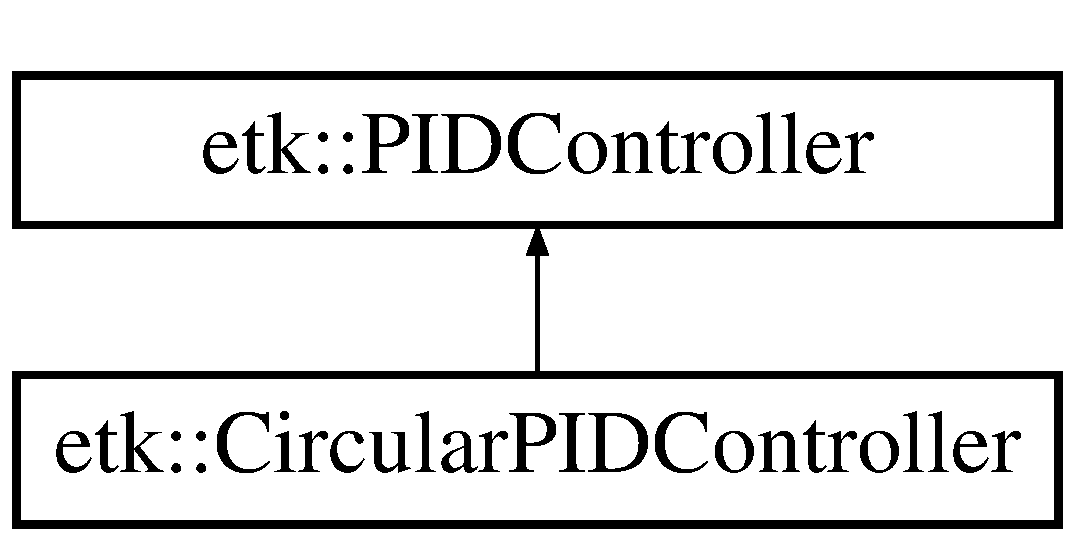
\includegraphics[height=2.000000cm]{classetk_1_1_circular_p_i_d_controller}
\end{center}
\end{figure}
\subsection*{Public Member Functions}
\begin{DoxyCompactItemize}
\item 
float \hyperlink{classetk_1_1_circular_p_i_d_controller_acefc7ea3b8ce7fbbf47a696753b48c24}{step} (float setpoint, float measurement, float segments, float dt)
\end{DoxyCompactItemize}
\subsection*{Additional Inherited Members}


\subsection{Detailed Description}
A Circular P\-I\-D Controller. This controller uses \hyperlink{namespaceetk_a0bb96bed2b97ddb4eba560684c0e050a}{constrain\-\_\-circular()}; to keep it's inputs and error within a circular range. If segments was set to 360, the setpoint was 175 and the measurement was -\/175, the resulting error would be -\/10 degrees. This makes the circular P\-I\-D controller suitable for controlling the heading of a vehicle, for example. 

\subsection{Member Function Documentation}
\hypertarget{classetk_1_1_circular_p_i_d_controller_acefc7ea3b8ce7fbbf47a696753b48c24}{\index{etk\-::\-Circular\-P\-I\-D\-Controller@{etk\-::\-Circular\-P\-I\-D\-Controller}!step@{step}}
\index{step@{step}!etk::CircularPIDController@{etk\-::\-Circular\-P\-I\-D\-Controller}}
\subsubsection[{step}]{\setlength{\rightskip}{0pt plus 5cm}float etk\-::\-Circular\-P\-I\-D\-Controller\-::step (
\begin{DoxyParamCaption}
\item[{float}]{setpoint, }
\item[{float}]{measurement, }
\item[{float}]{segments, }
\item[{float}]{dt}
\end{DoxyParamCaption}
)}}\label{classetk_1_1_circular_p_i_d_controller_acefc7ea3b8ce7fbbf47a696753b48c24}


The documentation for this class was generated from the following file\-:\begin{DoxyCompactItemize}
\item 
inc/etk/\hyperlink{pid_8h}{pid.\-h}\end{DoxyCompactItemize}

\hypertarget{classetk_1_1_coordinate}{\section{etk\-:\-:Coordinate Class Reference}
\label{classetk_1_1_coordinate}\index{etk\-::\-Coordinate@{etk\-::\-Coordinate}}
}


Represents latitude and longitude coordinates. Units are in degrees unless stated otherwise. All navigation functions use great circle mathematics and are, in theory, suitable for long distances and navigation in polar regions.  




{\ttfamily \#include $<$navigation.\-h$>$}

Inheritance diagram for etk\-:\-:Coordinate\-:\begin{figure}[H]
\begin{center}
\leavevmode
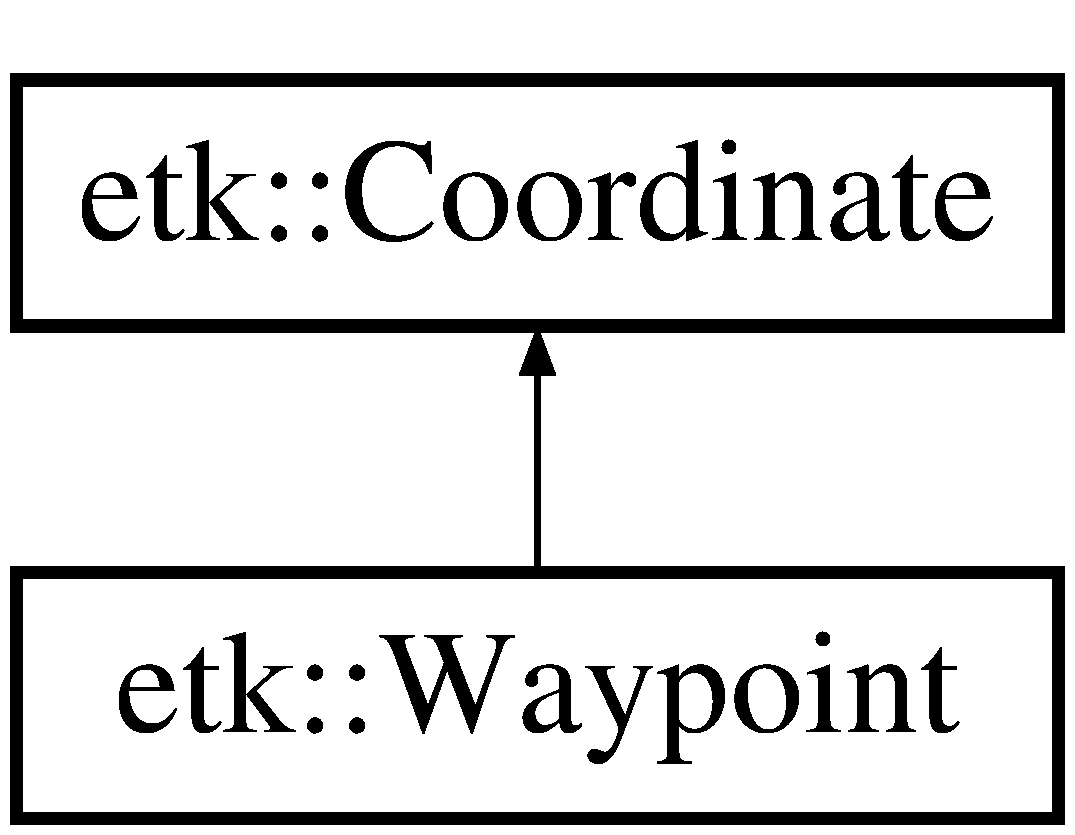
\includegraphics[height=2.000000cm]{classetk_1_1_coordinate}
\end{center}
\end{figure}
\subsection*{Public Member Functions}
\begin{DoxyCompactItemize}
\item 
\hyperlink{classetk_1_1_coordinate_a6f5e7ae3e170f4ced2e6917c4e59c9c9}{Coordinate} ()
\item 
\hyperlink{classetk_1_1_coordinate_a9e121c4f43995212e0c857bf3cf30c2a}{Coordinate} (float la, float ln)
\begin{DoxyCompactList}\small\item\em Creates a \hyperlink{classetk_1_1_coordinate}{Coordinate}. \end{DoxyCompactList}\item 
\hyperlink{classetk_1_1_coordinate_a61fb53571c35d863975d8b30d79a829e}{Coordinate} (\hyperlink{classetk_1_1_vector}{etk\-::\-Vector}$<$ 2 $>$ v)
\begin{DoxyCompactList}\small\item\em Creates a \hyperlink{classetk_1_1_coordinate}{Coordinate}. \end{DoxyCompactList}\item 
\hyperlink{classetk_1_1_coordinate_a5576579a2a9047c3fc7caa8063b5f94a}{Coordinate} (\hyperlink{classetk_1_1_vector}{etk\-::\-Vector}$<$ 3 $>$ v)
\begin{DoxyCompactList}\small\item\em Creates a \hyperlink{classetk_1_1_coordinate}{Coordinate}. \end{DoxyCompactList}\item 
float \hyperlink{classetk_1_1_coordinate_ad8e63194003e876f7e52e85d09a15cbb}{bearing\-\_\-to} (\hyperlink{classetk_1_1_coordinate}{Coordinate} to)
\begin{DoxyCompactList}\small\item\em Calculates the bearing to a coordinate. \end{DoxyCompactList}\item 
float \hyperlink{classetk_1_1_coordinate_afdc37e37396d5efd0ed16f76ee3df46d}{distance\-\_\-to} (\hyperlink{classetk_1_1_coordinate}{Coordinate} b)
\begin{DoxyCompactList}\small\item\em Calculates the distance to a coordinate. \end{DoxyCompactList}\item 
float \hyperlink{classetk_1_1_coordinate_a342706a6ba36f2d4349fd1b2eb32bd41}{cross\-\_\-track\-\_\-distance} (\hyperlink{classetk_1_1_coordinate}{Coordinate} from, \hyperlink{classetk_1_1_coordinate}{Coordinate} to)
\begin{DoxyCompactList}\small\item\em Calculates cross track distance (how far off course you are). \end{DoxyCompactList}\item 
\hyperlink{classetk_1_1_coordinate}{Coordinate} \hyperlink{classetk_1_1_coordinate_a11c15abf41756430aff34d666d8d13da}{destination\-\_\-from\-\_\-distance\-\_\-bearing} (float dist, float bearing)
\begin{DoxyCompactList}\small\item\em Given a distance and a bearing, this function calculates the destination coordinate. \end{DoxyCompactList}\item 
\hyperlink{classetk_1_1_coordinate_af0e3972f8bf38253cf2b40c79ac51300}{operator Vector$<$ 2 $>$} ()
\begin{DoxyCompactList}\small\item\em \hyperlink{classetk_1_1_coordinate}{Coordinate} can be seamlessly cast to a two dimensional vector. \end{DoxyCompactList}\item 
float \hyperlink{classetk_1_1_coordinate_afc991b2d2ba9e61e28c6784530f5b6ec}{get\-\_\-lat} ()
\begin{DoxyCompactList}\small\item\em Returns latitude. \end{DoxyCompactList}\item 
void \hyperlink{classetk_1_1_coordinate_aa9d7b6dbfdb4da3b788b88896edb6354}{set\-\_\-lat} (float l)
\begin{DoxyCompactList}\small\item\em Sets latitude. \end{DoxyCompactList}\item 
float \hyperlink{classetk_1_1_coordinate_ad59acdadf6fa7c597885f2248706c559}{get\-\_\-lng} ()
\begin{DoxyCompactList}\small\item\em Returns longitude. \end{DoxyCompactList}\item 
void \hyperlink{classetk_1_1_coordinate_a19d3ce4dab1e00903c0b609b4cf29fa2}{set\-\_\-lng} (float l)
\begin{DoxyCompactList}\small\item\em Sets longitude. \end{DoxyCompactList}\end{DoxyCompactItemize}
\subsection*{Protected Attributes}
\begin{DoxyCompactItemize}
\item 
float \hyperlink{classetk_1_1_coordinate_af261adfd9bac16c80b17046726d20c28}{lat} = 0
\item 
float \hyperlink{classetk_1_1_coordinate_a87145d8d5f3fb09f0cfc9e0d085aeda7}{lng} = 0
\end{DoxyCompactItemize}


\subsection{Detailed Description}
Represents latitude and longitude coordinates. Units are in degrees unless stated otherwise. All navigation functions use great circle mathematics and are, in theory, suitable for long distances and navigation in polar regions. 

\subsection{Constructor \& Destructor Documentation}
\hypertarget{classetk_1_1_coordinate_a6f5e7ae3e170f4ced2e6917c4e59c9c9}{\index{etk\-::\-Coordinate@{etk\-::\-Coordinate}!Coordinate@{Coordinate}}
\index{Coordinate@{Coordinate}!etk::Coordinate@{etk\-::\-Coordinate}}
\subsubsection[{Coordinate}]{\setlength{\rightskip}{0pt plus 5cm}etk\-::\-Coordinate\-::\-Coordinate (
\begin{DoxyParamCaption}
{}
\end{DoxyParamCaption}
)\hspace{0.3cm}{\ttfamily [inline]}}}\label{classetk_1_1_coordinate_a6f5e7ae3e170f4ced2e6917c4e59c9c9}
\hypertarget{classetk_1_1_coordinate_a9e121c4f43995212e0c857bf3cf30c2a}{\index{etk\-::\-Coordinate@{etk\-::\-Coordinate}!Coordinate@{Coordinate}}
\index{Coordinate@{Coordinate}!etk::Coordinate@{etk\-::\-Coordinate}}
\subsubsection[{Coordinate}]{\setlength{\rightskip}{0pt plus 5cm}etk\-::\-Coordinate\-::\-Coordinate (
\begin{DoxyParamCaption}
\item[{float}]{la, }
\item[{float}]{ln}
\end{DoxyParamCaption}
)}}\label{classetk_1_1_coordinate_a9e121c4f43995212e0c857bf3cf30c2a}


Creates a \hyperlink{classetk_1_1_coordinate}{Coordinate}. 

\begin{DoxyItemize}
\item la latitude \item ln longitude \end{DoxyItemize}
\hypertarget{classetk_1_1_coordinate_a61fb53571c35d863975d8b30d79a829e}{\index{etk\-::\-Coordinate@{etk\-::\-Coordinate}!Coordinate@{Coordinate}}
\index{Coordinate@{Coordinate}!etk::Coordinate@{etk\-::\-Coordinate}}
\subsubsection[{Coordinate}]{\setlength{\rightskip}{0pt plus 5cm}etk\-::\-Coordinate\-::\-Coordinate (
\begin{DoxyParamCaption}
\item[{{\bf etk\-::\-Vector}$<$ 2 $>$}]{v}
\end{DoxyParamCaption}
)}}\label{classetk_1_1_coordinate_a61fb53571c35d863975d8b30d79a829e}


Creates a \hyperlink{classetk_1_1_coordinate}{Coordinate}. 

\begin{DoxyItemize}
\item v A two dimensional vector with lat as x and lng as y. \end{DoxyItemize}
\hypertarget{classetk_1_1_coordinate_a5576579a2a9047c3fc7caa8063b5f94a}{\index{etk\-::\-Coordinate@{etk\-::\-Coordinate}!Coordinate@{Coordinate}}
\index{Coordinate@{Coordinate}!etk::Coordinate@{etk\-::\-Coordinate}}
\subsubsection[{Coordinate}]{\setlength{\rightskip}{0pt plus 5cm}etk\-::\-Coordinate\-::\-Coordinate (
\begin{DoxyParamCaption}
\item[{{\bf etk\-::\-Vector}$<$ 3 $>$}]{v}
\end{DoxyParamCaption}
)}}\label{classetk_1_1_coordinate_a5576579a2a9047c3fc7caa8063b5f94a}


Creates a \hyperlink{classetk_1_1_coordinate}{Coordinate}. 

\begin{DoxyItemize}
\item v A three dimensional vector with lat as x and lng as y. The z dimension is ignored. \end{DoxyItemize}


\subsection{Member Function Documentation}
\hypertarget{classetk_1_1_coordinate_ad8e63194003e876f7e52e85d09a15cbb}{\index{etk\-::\-Coordinate@{etk\-::\-Coordinate}!bearing\-\_\-to@{bearing\-\_\-to}}
\index{bearing\-\_\-to@{bearing\-\_\-to}!etk::Coordinate@{etk\-::\-Coordinate}}
\subsubsection[{bearing\-\_\-to}]{\setlength{\rightskip}{0pt plus 5cm}float etk\-::\-Coordinate\-::bearing\-\_\-to (
\begin{DoxyParamCaption}
\item[{{\bf Coordinate}}]{to}
\end{DoxyParamCaption}
)}}\label{classetk_1_1_coordinate_ad8e63194003e876f7e52e85d09a15cbb}


Calculates the bearing to a coordinate. 

\hypertarget{classetk_1_1_coordinate_a342706a6ba36f2d4349fd1b2eb32bd41}{\index{etk\-::\-Coordinate@{etk\-::\-Coordinate}!cross\-\_\-track\-\_\-distance@{cross\-\_\-track\-\_\-distance}}
\index{cross\-\_\-track\-\_\-distance@{cross\-\_\-track\-\_\-distance}!etk::Coordinate@{etk\-::\-Coordinate}}
\subsubsection[{cross\-\_\-track\-\_\-distance}]{\setlength{\rightskip}{0pt plus 5cm}float etk\-::\-Coordinate\-::cross\-\_\-track\-\_\-distance (
\begin{DoxyParamCaption}
\item[{{\bf Coordinate}}]{from, }
\item[{{\bf Coordinate}}]{to}
\end{DoxyParamCaption}
)}}\label{classetk_1_1_coordinate_a342706a6ba36f2d4349fd1b2eb32bd41}


Calculates cross track distance (how far off course you are). 

 \begin{DoxyReturn}{Returns}
Cross track distance in meters. 
\end{DoxyReturn}
\hypertarget{classetk_1_1_coordinate_a11c15abf41756430aff34d666d8d13da}{\index{etk\-::\-Coordinate@{etk\-::\-Coordinate}!destination\-\_\-from\-\_\-distance\-\_\-bearing@{destination\-\_\-from\-\_\-distance\-\_\-bearing}}
\index{destination\-\_\-from\-\_\-distance\-\_\-bearing@{destination\-\_\-from\-\_\-distance\-\_\-bearing}!etk::Coordinate@{etk\-::\-Coordinate}}
\subsubsection[{destination\-\_\-from\-\_\-distance\-\_\-bearing}]{\setlength{\rightskip}{0pt plus 5cm}{\bf Coordinate} etk\-::\-Coordinate\-::destination\-\_\-from\-\_\-distance\-\_\-bearing (
\begin{DoxyParamCaption}
\item[{float}]{dist, }
\item[{float}]{bearing}
\end{DoxyParamCaption}
)}}\label{classetk_1_1_coordinate_a11c15abf41756430aff34d666d8d13da}


Given a distance and a bearing, this function calculates the destination coordinate. 

\begin{DoxyItemize}
\item dist Distance in meters. \item bearing Direction to destination. \begin{DoxyReturn}{Returns}
\hyperlink{classetk_1_1_coordinate}{Coordinate} that represents the destination. 
\end{DoxyReturn}
\end{DoxyItemize}
\hypertarget{classetk_1_1_coordinate_afdc37e37396d5efd0ed16f76ee3df46d}{\index{etk\-::\-Coordinate@{etk\-::\-Coordinate}!distance\-\_\-to@{distance\-\_\-to}}
\index{distance\-\_\-to@{distance\-\_\-to}!etk::Coordinate@{etk\-::\-Coordinate}}
\subsubsection[{distance\-\_\-to}]{\setlength{\rightskip}{0pt plus 5cm}float etk\-::\-Coordinate\-::distance\-\_\-to (
\begin{DoxyParamCaption}
\item[{{\bf Coordinate}}]{b}
\end{DoxyParamCaption}
)}}\label{classetk_1_1_coordinate_afdc37e37396d5efd0ed16f76ee3df46d}


Calculates the distance to a coordinate. 

\begin{DoxyReturn}{Returns}
Distance to a coordinate in meters. 
\end{DoxyReturn}
\hypertarget{classetk_1_1_coordinate_afc991b2d2ba9e61e28c6784530f5b6ec}{\index{etk\-::\-Coordinate@{etk\-::\-Coordinate}!get\-\_\-lat@{get\-\_\-lat}}
\index{get\-\_\-lat@{get\-\_\-lat}!etk::Coordinate@{etk\-::\-Coordinate}}
\subsubsection[{get\-\_\-lat}]{\setlength{\rightskip}{0pt plus 5cm}float etk\-::\-Coordinate\-::get\-\_\-lat (
\begin{DoxyParamCaption}
{}
\end{DoxyParamCaption}
)\hspace{0.3cm}{\ttfamily [inline]}}}\label{classetk_1_1_coordinate_afc991b2d2ba9e61e28c6784530f5b6ec}


Returns latitude. 

\hypertarget{classetk_1_1_coordinate_ad59acdadf6fa7c597885f2248706c559}{\index{etk\-::\-Coordinate@{etk\-::\-Coordinate}!get\-\_\-lng@{get\-\_\-lng}}
\index{get\-\_\-lng@{get\-\_\-lng}!etk::Coordinate@{etk\-::\-Coordinate}}
\subsubsection[{get\-\_\-lng}]{\setlength{\rightskip}{0pt plus 5cm}float etk\-::\-Coordinate\-::get\-\_\-lng (
\begin{DoxyParamCaption}
{}
\end{DoxyParamCaption}
)\hspace{0.3cm}{\ttfamily [inline]}}}\label{classetk_1_1_coordinate_ad59acdadf6fa7c597885f2248706c559}


Returns longitude. 

\hypertarget{classetk_1_1_coordinate_af0e3972f8bf38253cf2b40c79ac51300}{\index{etk\-::\-Coordinate@{etk\-::\-Coordinate}!operator Vector$<$ 2 $>$@{operator Vector$<$ 2 $>$}}
\index{operator Vector$<$ 2 $>$@{operator Vector$<$ 2 $>$}!etk::Coordinate@{etk\-::\-Coordinate}}
\subsubsection[{operator Vector$<$ 2 $>$}]{\setlength{\rightskip}{0pt plus 5cm}etk\-::\-Coordinate\-::operator {\bf Vector}$<$ 2 $>$ (
\begin{DoxyParamCaption}
{}
\end{DoxyParamCaption}
)\hspace{0.3cm}{\ttfamily [inline]}}}\label{classetk_1_1_coordinate_af0e3972f8bf38253cf2b40c79ac51300}


\hyperlink{classetk_1_1_coordinate}{Coordinate} can be seamlessly cast to a two dimensional vector. 


\begin{DoxyCode}
\hyperlink{classetk_1_1_vector}{etk::Vector<2>} vec;
\hyperlink{classetk_1_1_coordinate}{etk::Coordinate} coord(5, 10);
vec = coord;
\end{DoxyCode}
 This makes it easy to perform more advanced vector mathematics on a coordinate. \hypertarget{classetk_1_1_coordinate_aa9d7b6dbfdb4da3b788b88896edb6354}{\index{etk\-::\-Coordinate@{etk\-::\-Coordinate}!set\-\_\-lat@{set\-\_\-lat}}
\index{set\-\_\-lat@{set\-\_\-lat}!etk::Coordinate@{etk\-::\-Coordinate}}
\subsubsection[{set\-\_\-lat}]{\setlength{\rightskip}{0pt plus 5cm}void etk\-::\-Coordinate\-::set\-\_\-lat (
\begin{DoxyParamCaption}
\item[{float}]{l}
\end{DoxyParamCaption}
)\hspace{0.3cm}{\ttfamily [inline]}}}\label{classetk_1_1_coordinate_aa9d7b6dbfdb4da3b788b88896edb6354}


Sets latitude. 

\hypertarget{classetk_1_1_coordinate_a19d3ce4dab1e00903c0b609b4cf29fa2}{\index{etk\-::\-Coordinate@{etk\-::\-Coordinate}!set\-\_\-lng@{set\-\_\-lng}}
\index{set\-\_\-lng@{set\-\_\-lng}!etk::Coordinate@{etk\-::\-Coordinate}}
\subsubsection[{set\-\_\-lng}]{\setlength{\rightskip}{0pt plus 5cm}void etk\-::\-Coordinate\-::set\-\_\-lng (
\begin{DoxyParamCaption}
\item[{float}]{l}
\end{DoxyParamCaption}
)\hspace{0.3cm}{\ttfamily [inline]}}}\label{classetk_1_1_coordinate_a19d3ce4dab1e00903c0b609b4cf29fa2}


Sets longitude. 



\subsection{Member Data Documentation}
\hypertarget{classetk_1_1_coordinate_af261adfd9bac16c80b17046726d20c28}{\index{etk\-::\-Coordinate@{etk\-::\-Coordinate}!lat@{lat}}
\index{lat@{lat}!etk::Coordinate@{etk\-::\-Coordinate}}
\subsubsection[{lat}]{\setlength{\rightskip}{0pt plus 5cm}float etk\-::\-Coordinate\-::lat = 0\hspace{0.3cm}{\ttfamily [protected]}}}\label{classetk_1_1_coordinate_af261adfd9bac16c80b17046726d20c28}
\hypertarget{classetk_1_1_coordinate_a87145d8d5f3fb09f0cfc9e0d085aeda7}{\index{etk\-::\-Coordinate@{etk\-::\-Coordinate}!lng@{lng}}
\index{lng@{lng}!etk::Coordinate@{etk\-::\-Coordinate}}
\subsubsection[{lng}]{\setlength{\rightskip}{0pt plus 5cm}float etk\-::\-Coordinate\-::lng = 0\hspace{0.3cm}{\ttfamily [protected]}}}\label{classetk_1_1_coordinate_a87145d8d5f3fb09f0cfc9e0d085aeda7}


The documentation for this class was generated from the following file\-:\begin{DoxyCompactItemize}
\item 
inc/etk/\hyperlink{navigation_8h}{navigation.\-h}\end{DoxyCompactItemize}

\input{classetk_1_1_evo_pid}
\hypertarget{classetk_1_1_expo_moving_avg}{\section{etk\-:\-:Expo\-Moving\-Avg Class Reference}
\label{classetk_1_1_expo_moving_avg}\index{etk\-::\-Expo\-Moving\-Avg@{etk\-::\-Expo\-Moving\-Avg}}
}


An exponential moving average low-\/pass filter.  




{\ttfamily \#include $<$filters.\-h$>$}

\subsection*{Public Member Functions}
\begin{DoxyCompactItemize}
\item 
\hyperlink{classetk_1_1_expo_moving_avg_a5194c9b3142d409ae109b66285c4fa60}{Expo\-Moving\-Avg} (real\-\_\-t f, real\-\_\-t init\-\_\-est=0)
\begin{DoxyCompactList}\small\item\em This constructor allows you to set the filter gain and initial estimate. \end{DoxyCompactList}\item 
void \hyperlink{classetk_1_1_expo_moving_avg_a772862fd59a243bba42d244311ee2643}{set\-\_\-gain} (real\-\_\-t factor)
\begin{DoxyCompactList}\small\item\em The gain controls the responsiveness of the filter. It should be a value between 0.\-0 and 1.\-0. A higher value makes the filter more responsive and allows more noise through. \end{DoxyCompactList}\item 
void \hyperlink{classetk_1_1_expo_moving_avg_a9e769e6b6f298d99f4329e1155fbe8bd}{step} (real\-\_\-t measurement)
\begin{DoxyCompactList}\small\item\em Performs a single iteration of the filter. Raw samples are entered into the filter using this function. \end{DoxyCompactList}\item 
\hypertarget{classetk_1_1_expo_moving_avg_a9a0fd1042f0a73282e3dbd4ef6d0353c}{real\-\_\-t \hyperlink{classetk_1_1_expo_moving_avg_a9a0fd1042f0a73282e3dbd4ef6d0353c}{get} ()}\label{classetk_1_1_expo_moving_avg_a9a0fd1042f0a73282e3dbd4ef6d0353c}

\begin{DoxyCompactList}\small\item\em Returns the current state of the filter. \end{DoxyCompactList}\end{DoxyCompactItemize}


\subsection{Detailed Description}
An exponential moving average low-\/pass filter. 


\begin{DoxyCode}
\hyperlink{classetk_1_1_expo_moving_avg}{etk::ExpoMovingAvg} filter(0.1);

\textcolor{keywordflow}{for}(\textcolor{keyword}{auto} i : \hyperlink{namespaceetk_aff39b0f367ee4d947e2e7d297ffd506b}{etk::range}(100))
\{
   filter.step(i);
   cout << filter.get() << endl;
\}
\end{DoxyCode}
 

\subsection{Constructor \& Destructor Documentation}
\hypertarget{classetk_1_1_expo_moving_avg_a5194c9b3142d409ae109b66285c4fa60}{\index{etk\-::\-Expo\-Moving\-Avg@{etk\-::\-Expo\-Moving\-Avg}!Expo\-Moving\-Avg@{Expo\-Moving\-Avg}}
\index{Expo\-Moving\-Avg@{Expo\-Moving\-Avg}!etk::ExpoMovingAvg@{etk\-::\-Expo\-Moving\-Avg}}
\subsubsection[{Expo\-Moving\-Avg}]{\setlength{\rightskip}{0pt plus 5cm}etk\-::\-Expo\-Moving\-Avg\-::\-Expo\-Moving\-Avg (
\begin{DoxyParamCaption}
\item[{real\-\_\-t}]{f, }
\item[{real\-\_\-t}]{init\-\_\-est = {\ttfamily 0}}
\end{DoxyParamCaption}
)\hspace{0.3cm}{\ttfamily [inline]}}}\label{classetk_1_1_expo_moving_avg_a5194c9b3142d409ae109b66285c4fa60}


This constructor allows you to set the filter gain and initial estimate. 

\begin{DoxyItemize}
\item f filter gain \item init\-\_\-est initial estimate \end{DoxyItemize}


\subsection{Member Function Documentation}
\hypertarget{classetk_1_1_expo_moving_avg_a772862fd59a243bba42d244311ee2643}{\index{etk\-::\-Expo\-Moving\-Avg@{etk\-::\-Expo\-Moving\-Avg}!set\-\_\-gain@{set\-\_\-gain}}
\index{set\-\_\-gain@{set\-\_\-gain}!etk::ExpoMovingAvg@{etk\-::\-Expo\-Moving\-Avg}}
\subsubsection[{set\-\_\-gain}]{\setlength{\rightskip}{0pt plus 5cm}void etk\-::\-Expo\-Moving\-Avg\-::set\-\_\-gain (
\begin{DoxyParamCaption}
\item[{real\-\_\-t}]{factor}
\end{DoxyParamCaption}
)\hspace{0.3cm}{\ttfamily [inline]}}}\label{classetk_1_1_expo_moving_avg_a772862fd59a243bba42d244311ee2643}


The gain controls the responsiveness of the filter. It should be a value between 0.\-0 and 1.\-0. A higher value makes the filter more responsive and allows more noise through. 

\begin{DoxyItemize}
\item factor The filter gain (0.\-0 -\/ 1.\-0) \end{DoxyItemize}
\hypertarget{classetk_1_1_expo_moving_avg_a9e769e6b6f298d99f4329e1155fbe8bd}{\index{etk\-::\-Expo\-Moving\-Avg@{etk\-::\-Expo\-Moving\-Avg}!step@{step}}
\index{step@{step}!etk::ExpoMovingAvg@{etk\-::\-Expo\-Moving\-Avg}}
\subsubsection[{step}]{\setlength{\rightskip}{0pt plus 5cm}void etk\-::\-Expo\-Moving\-Avg\-::step (
\begin{DoxyParamCaption}
\item[{real\-\_\-t}]{measurement}
\end{DoxyParamCaption}
)\hspace{0.3cm}{\ttfamily [inline]}}}\label{classetk_1_1_expo_moving_avg_a9e769e6b6f298d99f4329e1155fbe8bd}


Performs a single iteration of the filter. Raw samples are entered into the filter using this function. 

\begin{DoxyItemize}
\item measurement A raw measurement or sample to be filtered. \end{DoxyItemize}


The documentation for this class was generated from the following file\-:\begin{DoxyCompactItemize}
\item 
inc/etk/filters.\-h\end{DoxyCompactItemize}

\hypertarget{classetk_1_1_fuzzy}{\section{etk\-:\-:Fuzzy$<$ N $>$ Class Template Reference}
\label{classetk_1_1_fuzzy}\index{etk\-::\-Fuzzy$<$ N $>$@{etk\-::\-Fuzzy$<$ N $>$}}
}


\hyperlink{classetk_1_1_fuzzy}{Fuzzy} logic class. \hyperlink{classetk_1_1_fuzzy}{Fuzzy} logic can be used for function approximation, control applications, signal process, A\-I and so on. Here is a tutorial on using \hyperlink{classetk_1_1_fuzzy}{Fuzzy} logic with E\-T\-K \href{http://www.camelsoftware.com/blog/2015/12/12/fuzzy-logic-control-part-1/}{\tt http\-://www.\-camelsoftware.\-com/blog/2015/12/12/fuzzy-\/logic-\/control-\/part-\/1/}.  




{\ttfamily \#include $<$fuzzy.\-h$>$}

\subsection*{Classes}
\begin{DoxyCompactItemize}
\item 
class \hyperlink{classetk_1_1_fuzzy_1_1_set}{Set}
\begin{DoxyCompactList}\small\item\em A fuzzy logic set. \end{DoxyCompactList}\end{DoxyCompactItemize}
\subsection*{Public Member Functions}
\begin{DoxyCompactItemize}
\item 
\hypertarget{classetk_1_1_fuzzy_abe817aa98e6ad63a9d0f9d28aa917d7a}{void \hyperlink{classetk_1_1_fuzzy_abe817aa98e6ad63a9d0f9d28aa917d7a}{add\-\_\-set} (\hyperlink{classetk_1_1_fuzzy_1_1_set}{Set} \&f)}\label{classetk_1_1_fuzzy_abe817aa98e6ad63a9d0f9d28aa917d7a}

\begin{DoxyCompactList}\small\item\em Adds a set. You can add up to N sets. \end{DoxyCompactList}\item 
\hypertarget{classetk_1_1_fuzzy_a2d10f9ca458595dfb404094903eb82e3}{uint32 \hyperlink{classetk_1_1_fuzzy_a2d10f9ca458595dfb404094903eb82e3}{get\-\_\-n\-\_\-sets} ()}\label{classetk_1_1_fuzzy_a2d10f9ca458595dfb404094903eb82e3}

\begin{DoxyCompactList}\small\item\em Returns the number of sets. \end{DoxyCompactList}\item 
\hypertarget{classetk_1_1_fuzzy_a000d2dcf15ab0aa1d6cb9b7a528c2ed4}{void \hyperlink{classetk_1_1_fuzzy_a000d2dcf15ab0aa1d6cb9b7a528c2ed4}{clear\-\_\-sets} ()}\label{classetk_1_1_fuzzy_a000d2dcf15ab0aa1d6cb9b7a528c2ed4}

\begin{DoxyCompactList}\small\item\em Removes all sets. \end{DoxyCompactList}\item 
real\-\_\-t \hyperlink{classetk_1_1_fuzzy_a5034d3a6a627d478e65ceade3b8a6171}{crisp\-\_\-out} (real\-\_\-t crisp\-\_\-in)
\begin{DoxyCompactList}\small\item\em Returns a crisp output for a given crisp input. \end{DoxyCompactList}\item 
auto \hyperlink{classetk_1_1_fuzzy_a4a4952392e6950a71734304a8b880fab}{inverse} ()
\begin{DoxyCompactList}\small\item\em Returns a fuzzy logic class that is inverted. Let's say you're using \hyperlink{classetk_1_1_fuzzy}{Fuzzy} to control speed using throttle. You know for throttle x you get speed y. You can plot the throttle response using \hyperlink{classetk_1_1_fuzzy}{Fuzzy}, but all that's going to tell is you what speed to expect for a selected throttle setting. By inverting the \hyperlink{classetk_1_1_fuzzy}{Fuzzy} sets, you can work backwards and determine what throttle setting is required for a selected speed. \end{DoxyCompactList}\end{DoxyCompactItemize}


\subsection{Detailed Description}
\subsubsection*{template$<$uint16 N$>$class etk\-::\-Fuzzy$<$ N $>$}

\hyperlink{classetk_1_1_fuzzy}{Fuzzy} logic class. \hyperlink{classetk_1_1_fuzzy}{Fuzzy} logic can be used for function approximation, control applications, signal process, A\-I and so on. Here is a tutorial on using \hyperlink{classetk_1_1_fuzzy}{Fuzzy} logic with E\-T\-K \href{http://www.camelsoftware.com/blog/2015/12/12/fuzzy-logic-control-part-1/}{\tt http\-://www.\-camelsoftware.\-com/blog/2015/12/12/fuzzy-\/logic-\/control-\/part-\/1/}. 


\begin{DoxyTemplParams}{Template Parameters}
{\em N} & The maximum number of fuzzy sets to use. \\
\hline
\end{DoxyTemplParams}


\subsection{Member Function Documentation}
\hypertarget{classetk_1_1_fuzzy_a5034d3a6a627d478e65ceade3b8a6171}{\index{etk\-::\-Fuzzy@{etk\-::\-Fuzzy}!crisp\-\_\-out@{crisp\-\_\-out}}
\index{crisp\-\_\-out@{crisp\-\_\-out}!etk::Fuzzy@{etk\-::\-Fuzzy}}
\subsubsection[{crisp\-\_\-out}]{\setlength{\rightskip}{0pt plus 5cm}template$<$uint16 N$>$ real\-\_\-t {\bf etk\-::\-Fuzzy}$<$ N $>$\-::crisp\-\_\-out (
\begin{DoxyParamCaption}
\item[{real\-\_\-t}]{crisp\-\_\-in}
\end{DoxyParamCaption}
)\hspace{0.3cm}{\ttfamily [inline]}}}\label{classetk_1_1_fuzzy_a5034d3a6a627d478e65ceade3b8a6171}


Returns a crisp output for a given crisp input. 

\begin{DoxyItemize}
\item crisp\-\_\-in A crisp input. \begin{DoxyReturn}{Returns}
A crisp output. 
\end{DoxyReturn}
\end{DoxyItemize}
\hypertarget{classetk_1_1_fuzzy_a4a4952392e6950a71734304a8b880fab}{\index{etk\-::\-Fuzzy@{etk\-::\-Fuzzy}!inverse@{inverse}}
\index{inverse@{inverse}!etk::Fuzzy@{etk\-::\-Fuzzy}}
\subsubsection[{inverse}]{\setlength{\rightskip}{0pt plus 5cm}template$<$uint16 N$>$ auto {\bf etk\-::\-Fuzzy}$<$ N $>$\-::inverse (
\begin{DoxyParamCaption}
{}
\end{DoxyParamCaption}
)\hspace{0.3cm}{\ttfamily [inline]}}}\label{classetk_1_1_fuzzy_a4a4952392e6950a71734304a8b880fab}


Returns a fuzzy logic class that is inverted. Let's say you're using \hyperlink{classetk_1_1_fuzzy}{Fuzzy} to control speed using throttle. You know for throttle x you get speed y. You can plot the throttle response using \hyperlink{classetk_1_1_fuzzy}{Fuzzy}, but all that's going to tell is you what speed to expect for a selected throttle setting. By inverting the \hyperlink{classetk_1_1_fuzzy}{Fuzzy} sets, you can work backwards and determine what throttle setting is required for a selected speed. 

\begin{DoxyReturn}{Returns}
A \hyperlink{classetk_1_1_fuzzy}{Fuzzy} class that plots an inverse function. 
\end{DoxyReturn}


The documentation for this class was generated from the following file\-:\begin{DoxyCompactItemize}
\item 
inc/etk/fuzzy.\-h\end{DoxyCompactItemize}

\hypertarget{classetk_1_1_high_pass_filter}{\section{etk\-:\-:High\-Pass\-Filter Class Reference}
\label{classetk_1_1_high_pass_filter}\index{etk\-::\-High\-Pass\-Filter@{etk\-::\-High\-Pass\-Filter}}
}


The \hyperlink{classetk_1_1_high_pass_filter}{High\-Pass\-Filter} blocks long term averages and allows higher frequencies through.  




{\ttfamily \#include $<$filters.\-h$>$}

\subsection*{Public Member Functions}
\begin{DoxyCompactItemize}
\item 
\hypertarget{classetk_1_1_high_pass_filter_ab909bdafbb6c61c4aea3cc8992542285}{\hyperlink{classetk_1_1_high_pass_filter_ab909bdafbb6c61c4aea3cc8992542285}{High\-Pass\-Filter} (real\-\_\-t gain)}\label{classetk_1_1_high_pass_filter_ab909bdafbb6c61c4aea3cc8992542285}

\begin{DoxyCompactList}\small\item\em The gain is set by the constructor. The gain must be between 0.\-0 and 1.\-0. The higher the gain, the higher the cutoff frequency. \end{DoxyCompactList}\item 
void \hyperlink{classetk_1_1_high_pass_filter_a679d243641f3ab15eba34cd5e3a64d18}{step} (real\-\_\-t sample)
\begin{DoxyCompactList}\small\item\em Performs a single iteration of the filter. Raw samples are entered into the filter using this function. \end{DoxyCompactList}\item 
\hypertarget{classetk_1_1_high_pass_filter_a19431d355cd6bd350d4603e31a0cedcf}{real\-\_\-t \hyperlink{classetk_1_1_high_pass_filter_a19431d355cd6bd350d4603e31a0cedcf}{get} ()}\label{classetk_1_1_high_pass_filter_a19431d355cd6bd350d4603e31a0cedcf}

\begin{DoxyCompactList}\small\item\em Returns the current state of the filter. \end{DoxyCompactList}\end{DoxyCompactItemize}


\subsection{Detailed Description}
The \hyperlink{classetk_1_1_high_pass_filter}{High\-Pass\-Filter} blocks long term averages and allows higher frequencies through. 

\subsection{Member Function Documentation}
\hypertarget{classetk_1_1_high_pass_filter_a679d243641f3ab15eba34cd5e3a64d18}{\index{etk\-::\-High\-Pass\-Filter@{etk\-::\-High\-Pass\-Filter}!step@{step}}
\index{step@{step}!etk::HighPassFilter@{etk\-::\-High\-Pass\-Filter}}
\subsubsection[{step}]{\setlength{\rightskip}{0pt plus 5cm}void etk\-::\-High\-Pass\-Filter\-::step (
\begin{DoxyParamCaption}
\item[{real\-\_\-t}]{sample}
\end{DoxyParamCaption}
)\hspace{0.3cm}{\ttfamily [inline]}}}\label{classetk_1_1_high_pass_filter_a679d243641f3ab15eba34cd5e3a64d18}


Performs a single iteration of the filter. Raw samples are entered into the filter using this function. 

\begin{DoxyItemize}
\item measurement A raw measurement or sample to be filtered. \end{DoxyItemize}


The documentation for this class was generated from the following file\-:\begin{DoxyCompactItemize}
\item 
inc/etk/filters.\-h\end{DoxyCompactItemize}

\hypertarget{classetk_1_1_short_term_memory_1_1_iterator}{\section{etk\-:\-:Short\-Term\-Memory$<$ T, L\-E\-N $>$\-:\-:Iterator Class Reference}
\label{classetk_1_1_short_term_memory_1_1_iterator}\index{etk\-::\-Short\-Term\-Memory$<$ T, L\-E\-N $>$\-::\-Iterator@{etk\-::\-Short\-Term\-Memory$<$ T, L\-E\-N $>$\-::\-Iterator}}
}
\subsection*{Public Member Functions}
\begin{DoxyCompactItemize}
\item 
\hypertarget{classetk_1_1_short_term_memory_1_1_iterator_abcfe12dc44a7f81335898956df39a653}{{\bfseries Iterator} (\hyperlink{classetk_1_1_short_term_memory}{Short\-Term\-Memory}$<$ T, L\-E\-N $>$ \&p, uint32 position=0)}\label{classetk_1_1_short_term_memory_1_1_iterator_abcfe12dc44a7f81335898956df39a653}

\item 
\hypertarget{classetk_1_1_short_term_memory_1_1_iterator_ae0dad866d5927d8ee3d9717a178427e8}{T {\bfseries operator$\ast$} ()}\label{classetk_1_1_short_term_memory_1_1_iterator_ae0dad866d5927d8ee3d9717a178427e8}

\item 
\hypertarget{classetk_1_1_short_term_memory_1_1_iterator_ae5d8621f94f142690d5d2bd50aa3d8af}{\hyperlink{classetk_1_1_short_term_memory_1_1_iterator}{Iterator} \& {\bfseries operator++} ()}\label{classetk_1_1_short_term_memory_1_1_iterator_ae5d8621f94f142690d5d2bd50aa3d8af}

\item 
\hypertarget{classetk_1_1_short_term_memory_1_1_iterator_a18c7ce8f9a1b98ffec26f6be66fa54b0}{bool {\bfseries operator==} (\hyperlink{classetk_1_1_short_term_memory_1_1_iterator}{Iterator} iter)}\label{classetk_1_1_short_term_memory_1_1_iterator_a18c7ce8f9a1b98ffec26f6be66fa54b0}

\item 
\hypertarget{classetk_1_1_short_term_memory_1_1_iterator_aee6649ed22232dae992b18a2386a8893}{bool {\bfseries operator!=} (\hyperlink{classetk_1_1_short_term_memory_1_1_iterator}{Iterator} iter)}\label{classetk_1_1_short_term_memory_1_1_iterator_aee6649ed22232dae992b18a2386a8893}

\end{DoxyCompactItemize}


The documentation for this class was generated from the following file\-:\begin{DoxyCompactItemize}
\item 
inc/etk/stm.\-h\end{DoxyCompactItemize}

\input{classetk_1_1_array_1_1_iterator}
\hypertarget{classetk_1_1_list_1_1_iterator}{\section{etk\-:\-:List$<$ T, L $>$\-:\-:Iterator Class Reference}
\label{classetk_1_1_list_1_1_iterator}\index{etk\-::\-List$<$ T, L $>$\-::\-Iterator@{etk\-::\-List$<$ T, L $>$\-::\-Iterator}}
}


The list iterator makes a list iterable using C++11 ranged for loop syntax.  




{\ttfamily \#include $<$list.\-h$>$}

\subsection*{Public Member Functions}
\begin{DoxyCompactItemize}
\item 
\hypertarget{classetk_1_1_list_1_1_iterator_a6a299eafca46db90564fdbffca60c7fa}{{\bfseries Iterator} (\hyperlink{classetk_1_1_list}{List} \&list)}\label{classetk_1_1_list_1_1_iterator_a6a299eafca46db90564fdbffca60c7fa}

\item 
\hypertarget{classetk_1_1_list_1_1_iterator_a368d2b78fd175b0dac43aee52dc54f8f}{T \& {\bfseries operator$\ast$} ()}\label{classetk_1_1_list_1_1_iterator_a368d2b78fd175b0dac43aee52dc54f8f}

\item 
\hypertarget{classetk_1_1_list_1_1_iterator_aa7b714a588a29db93f9e406223b8783c}{\hyperlink{classetk_1_1_list_1_1_iterator}{Iterator} \& {\bfseries operator++} ()}\label{classetk_1_1_list_1_1_iterator_aa7b714a588a29db93f9e406223b8783c}

\item 
\hypertarget{classetk_1_1_list_1_1_iterator_ae1f9efc5598a14487881bd7281fd27dd}{\hyperlink{classetk_1_1_list_1_1_iterator}{Iterator} {\bfseries operator++} (int)}\label{classetk_1_1_list_1_1_iterator_ae1f9efc5598a14487881bd7281fd27dd}

\item 
\hypertarget{classetk_1_1_list_1_1_iterator_a971c5acbef70bdd9a9513a87ad40fd4e}{bool {\bfseries operator==} (\hyperlink{classetk_1_1_list_1_1_iterator}{Iterator} iter)}\label{classetk_1_1_list_1_1_iterator_a971c5acbef70bdd9a9513a87ad40fd4e}

\item 
\hypertarget{classetk_1_1_list_1_1_iterator_a7c9b29d64794609438e68b928125f14b}{bool {\bfseries operator!=} (\hyperlink{classetk_1_1_list_1_1_iterator}{Iterator} iter)}\label{classetk_1_1_list_1_1_iterator_a7c9b29d64794609438e68b928125f14b}

\end{DoxyCompactItemize}
\subsection*{Friends}
\begin{DoxyCompactItemize}
\item 
\hypertarget{classetk_1_1_list_1_1_iterator_a8cee552d09eaeb60a09d95309a87b498}{class {\bfseries List}}\label{classetk_1_1_list_1_1_iterator_a8cee552d09eaeb60a09d95309a87b498}

\end{DoxyCompactItemize}


\subsection{Detailed Description}
\subsubsection*{template$<$typename T, uint32 L$>$class etk\-::\-List$<$ T, L $>$\-::\-Iterator}

The list iterator makes a list iterable using C++11 ranged for loop syntax. 


\begin{DoxyCode}
\hyperlink{classetk_1_1_list}{etk::List<int, 10>} list;
...
\textcolor{comment}{//print out the entire list}
for(\textcolor{keyword}{auto} i : list)
\{
    cout << i << \textcolor{stringliteral}{" "};
\}
\end{DoxyCode}
 

The documentation for this class was generated from the following file\-:\begin{DoxyCompactItemize}
\item 
inc/etk/list.\-h\end{DoxyCompactItemize}

\hypertarget{classetk_1_1_list}{\section{etk\-:\-:List$<$ T, L $>$ Class Template Reference}
\label{classetk_1_1_list}\index{etk\-::\-List$<$ T, L $>$@{etk\-::\-List$<$ T, L $>$}}
}


The list class is an iterable container object. A list can contain up to a maximum number of items determined by the template parameter L. \hyperlink{classetk_1_1_list}{List} is supposed to provide a similar look and feel to std\-::vector, but without using dynamic memory allocation.  




{\ttfamily \#include $<$list.\-h$>$}

\subsection*{Classes}
\begin{DoxyCompactItemize}
\item 
class \hyperlink{classetk_1_1_list_1_1_iterator}{Iterator}
\begin{DoxyCompactList}\small\item\em The list iterator makes a list iterable using C++11 ranged for loop syntax. \end{DoxyCompactList}\end{DoxyCompactItemize}
\subsection*{Public Member Functions}
\begin{DoxyCompactItemize}
\item 
\hypertarget{classetk_1_1_list_a23f9b0efe027159f914214d126b486b3}{{\bfseries List} (\hyperlink{classetk_1_1_list}{List} \&list)}\label{classetk_1_1_list_a23f9b0efe027159f914214d126b486b3}

\item 
\hypertarget{classetk_1_1_list_ac85e0e37f248ba1b52f410cd00c8c304}{{\bfseries List} (const \hyperlink{classetk_1_1_list}{List} \&list)}\label{classetk_1_1_list_ac85e0e37f248ba1b52f410cd00c8c304}

\item 
\hypertarget{classetk_1_1_list_afb70c4551d2e9ebc6b4bb04337d081e6}{\hyperlink{classetk_1_1_list_1_1_iterator}{Iterator} \hyperlink{classetk_1_1_list_afb70c4551d2e9ebc6b4bb04337d081e6}{begin} ()}\label{classetk_1_1_list_afb70c4551d2e9ebc6b4bb04337d081e6}

\begin{DoxyCompactList}\small\item\em Returns an iterator to the first item in the list. \end{DoxyCompactList}\item 
\hypertarget{classetk_1_1_list_a19b25cd89872debc07cc002c18845578}{\hyperlink{classetk_1_1_list_1_1_iterator}{Iterator} \hyperlink{classetk_1_1_list_a19b25cd89872debc07cc002c18845578}{end} ()}\label{classetk_1_1_list_a19b25cd89872debc07cc002c18845578}

\begin{DoxyCompactList}\small\item\em Returns an iterator to the end of the list. \end{DoxyCompactList}\item 
\hypertarget{classetk_1_1_list_a45df48bc3bb87c2dd26e56f51115ab27}{void \hyperlink{classetk_1_1_list_a45df48bc3bb87c2dd26e56f51115ab27}{append} (T t)}\label{classetk_1_1_list_a45df48bc3bb87c2dd26e56f51115ab27}

\begin{DoxyCompactList}\small\item\em Adds an item to the end of the list and increments the size of the list by 1. \end{DoxyCompactList}\item 
void \hyperlink{classetk_1_1_list_a95d6852055e5669632da51c6aa60e949}{insert} (T t, uint32 pos)
\begin{DoxyCompactList}\small\item\em Inserts an item into the list. \end{DoxyCompactList}\item 
void \hyperlink{classetk_1_1_list_a720fec604f6c57135b6796167171756a}{remove} (uint32 pos)
\begin{DoxyCompactList}\small\item\em Removes an item from the list. \end{DoxyCompactList}\item 
\hypertarget{classetk_1_1_list_a2b922183cf60d1bf3c351af927cfe51d}{void {\bfseries remove\-\_\-item} (auto \&item)}\label{classetk_1_1_list_a2b922183cf60d1bf3c351af927cfe51d}

\item 
void \hyperlink{classetk_1_1_list_a1e3a92350967e1fabcda37bbef21b796}{erase} (uint32 pos, uint32 len)
\begin{DoxyCompactList}\small\item\em Removes len number of items from the list, starting as pos. \end{DoxyCompactList}\item 
\hypertarget{classetk_1_1_list_a429128ca6b0d5f9e97fdfd52b0190364}{void \hyperlink{classetk_1_1_list_a429128ca6b0d5f9e97fdfd52b0190364}{clear} ()}\label{classetk_1_1_list_a429128ca6b0d5f9e97fdfd52b0190364}

\begin{DoxyCompactList}\small\item\em Destroys every item in the list. \end{DoxyCompactList}\item 
uint32 \hyperlink{classetk_1_1_list_a27f50a1845850dd0f19397e4e1bafe08}{count} (T t)
\begin{DoxyCompactList}\small\item\em Returns the number of a particular item in the list. \end{DoxyCompactList}\item 
void \hyperlink{classetk_1_1_list_aa21f417c80d9d8eeed6f33ed5c4af285}{fill} (uint32 start, uint32 \hyperlink{classetk_1_1_list_a19b25cd89872debc07cc002c18845578}{end}, T f)
\begin{DoxyCompactList}\small\item\em Sets a section of the list to a given value. \end{DoxyCompactList}\item 
T \hyperlink{classetk_1_1_list_a85741b89a92238cce95b940ce8a5554e}{pop\-\_\-back} ()
\begin{DoxyCompactList}\small\item\em Returns the last item on the list and reduces the list length by 1. \end{DoxyCompactList}\item 
\hypertarget{classetk_1_1_list_ab7dc844f7e80ac5ea9e7a8923230385a}{void \hyperlink{classetk_1_1_list_ab7dc844f7e80ac5ea9e7a8923230385a}{push\-\_\-back} (T t)}\label{classetk_1_1_list_ab7dc844f7e80ac5ea9e7a8923230385a}

\begin{DoxyCompactList}\small\item\em Same as \hyperlink{classetk_1_1_list_a45df48bc3bb87c2dd26e56f51115ab27}{append()};. \end{DoxyCompactList}\item 
\hypertarget{classetk_1_1_list_acc341d1d8b1b29b7868024777ef15b04}{T \& \hyperlink{classetk_1_1_list_acc341d1d8b1b29b7868024777ef15b04}{operator\mbox{[}$\,$\mbox{]}} (uint32 pos)}\label{classetk_1_1_list_acc341d1d8b1b29b7868024777ef15b04}

\begin{DoxyCompactList}\small\item\em This operator allows you to access elements of the list just like a normal array. \end{DoxyCompactList}\item 
\hypertarget{classetk_1_1_list_aa69eac1c25dcbdedff7f5ce2b7fcaff1}{uint32 \hyperlink{classetk_1_1_list_aa69eac1c25dcbdedff7f5ce2b7fcaff1}{size} ()}\label{classetk_1_1_list_aa69eac1c25dcbdedff7f5ce2b7fcaff1}

\begin{DoxyCompactList}\small\item\em Returns the number of items in the list. \end{DoxyCompactList}\item 
\hypertarget{classetk_1_1_list_af38a32c25ece381c033d9013141a0f12}{uint32 \hyperlink{classetk_1_1_list_af38a32c25ece381c033d9013141a0f12}{max\-\_\-len} ()}\label{classetk_1_1_list_af38a32c25ece381c033d9013141a0f12}

\begin{DoxyCompactList}\small\item\em Returns the maximum possible number of items that the list can contain. \end{DoxyCompactList}\item 
\hypertarget{classetk_1_1_list_ae5ff761960ef80143162ac2d4cd6a456}{void \hyperlink{classetk_1_1_list_ae5ff761960ef80143162ac2d4cd6a456}{set\-\_\-list\-\_\-end} (uint32 le)}\label{classetk_1_1_list_ae5ff761960ef80143162ac2d4cd6a456}

\begin{DoxyCompactList}\small\item\em Overrides the list end pointer. This function can be convenient but should be used with caution. \end{DoxyCompactList}\item 
\hypertarget{classetk_1_1_list_a765da91f522c96c94efec3790b5a63b5}{const T $\ast$ \hyperlink{classetk_1_1_list_a765da91f522c96c94efec3790b5a63b5}{buffer} () const }\label{classetk_1_1_list_a765da91f522c96c94efec3790b5a63b5}

\begin{DoxyCompactList}\small\item\em Returns a const pointer to the array. \end{DoxyCompactList}\item 
\hypertarget{classetk_1_1_list_add87c29d6b7283b6329a01c3b1eae898}{T $\ast$ \hyperlink{classetk_1_1_list_add87c29d6b7283b6329a01c3b1eae898}{raw\-\_\-memory} ()}\label{classetk_1_1_list_add87c29d6b7283b6329a01c3b1eae898}

\begin{DoxyCompactList}\small\item\em Returns a pointer to the raw memory used by \hyperlink{classetk_1_1_list}{List}. \end{DoxyCompactList}\end{DoxyCompactItemize}


\subsection{Detailed Description}
\subsubsection*{template$<$typename T, uint32 L$>$class etk\-::\-List$<$ T, L $>$}

The list class is an iterable container object. A list can contain up to a maximum number of items determined by the template parameter L. \hyperlink{classetk_1_1_list}{List} is supposed to provide a similar look and feel to std\-::vector, but without using dynamic memory allocation. 


\begin{DoxyTemplParams}{Template Parameters}
{\em T} & The type of object that the list contains. \\
\hline
{\em L} & The maximum size of the list. \\
\hline
\end{DoxyTemplParams}


\subsection{Member Function Documentation}
\hypertarget{classetk_1_1_list_a27f50a1845850dd0f19397e4e1bafe08}{\index{etk\-::\-List@{etk\-::\-List}!count@{count}}
\index{count@{count}!etk::List@{etk\-::\-List}}
\subsubsection[{count}]{\setlength{\rightskip}{0pt plus 5cm}template$<$typename T, uint32 L$>$ uint32 {\bf etk\-::\-List}$<$ T, L $>$\-::count (
\begin{DoxyParamCaption}
\item[{T}]{t}
\end{DoxyParamCaption}
)\hspace{0.3cm}{\ttfamily [inline]}}}\label{classetk_1_1_list_a27f50a1845850dd0f19397e4e1bafe08}


Returns the number of a particular item in the list. 

\begin{DoxyItemize}
\item t The item to count. \begin{DoxyReturn}{Returns}
The number of these items in the list. 
\end{DoxyReturn}
\end{DoxyItemize}
\hypertarget{classetk_1_1_list_a1e3a92350967e1fabcda37bbef21b796}{\index{etk\-::\-List@{etk\-::\-List}!erase@{erase}}
\index{erase@{erase}!etk::List@{etk\-::\-List}}
\subsubsection[{erase}]{\setlength{\rightskip}{0pt plus 5cm}template$<$typename T, uint32 L$>$ void {\bf etk\-::\-List}$<$ T, L $>$\-::erase (
\begin{DoxyParamCaption}
\item[{uint32}]{pos, }
\item[{uint32}]{len}
\end{DoxyParamCaption}
)\hspace{0.3cm}{\ttfamily [inline]}}}\label{classetk_1_1_list_a1e3a92350967e1fabcda37bbef21b796}


Removes len number of items from the list, starting as pos. 

\begin{DoxyItemize}
\item pos The position of the first item to erase. \item len The number of items to remove. \end{DoxyItemize}
\hypertarget{classetk_1_1_list_aa21f417c80d9d8eeed6f33ed5c4af285}{\index{etk\-::\-List@{etk\-::\-List}!fill@{fill}}
\index{fill@{fill}!etk::List@{etk\-::\-List}}
\subsubsection[{fill}]{\setlength{\rightskip}{0pt plus 5cm}template$<$typename T, uint32 L$>$ void {\bf etk\-::\-List}$<$ T, L $>$\-::fill (
\begin{DoxyParamCaption}
\item[{uint32}]{start, }
\item[{uint32}]{end, }
\item[{T}]{f}
\end{DoxyParamCaption}
)\hspace{0.3cm}{\ttfamily [inline]}}}\label{classetk_1_1_list_aa21f417c80d9d8eeed6f33ed5c4af285}


Sets a section of the list to a given value. 

\begin{DoxyItemize}
\item start The starting position. \item end The end position. \item f The item to fill with. \end{DoxyItemize}
\hypertarget{classetk_1_1_list_a95d6852055e5669632da51c6aa60e949}{\index{etk\-::\-List@{etk\-::\-List}!insert@{insert}}
\index{insert@{insert}!etk::List@{etk\-::\-List}}
\subsubsection[{insert}]{\setlength{\rightskip}{0pt plus 5cm}template$<$typename T, uint32 L$>$ void {\bf etk\-::\-List}$<$ T, L $>$\-::insert (
\begin{DoxyParamCaption}
\item[{T}]{t, }
\item[{uint32}]{pos}
\end{DoxyParamCaption}
)\hspace{0.3cm}{\ttfamily [inline]}}}\label{classetk_1_1_list_a95d6852055e5669632da51c6aa60e949}


Inserts an item into the list. 

\begin{DoxyItemize}
\item T the item to be inserted. \item pos where the item will be inserted. If pos is zero, then it will be inserted at the start of the list. If it's 1, it will become the second item in the list. \end{DoxyItemize}
\hypertarget{classetk_1_1_list_a85741b89a92238cce95b940ce8a5554e}{\index{etk\-::\-List@{etk\-::\-List}!pop\-\_\-back@{pop\-\_\-back}}
\index{pop\-\_\-back@{pop\-\_\-back}!etk::List@{etk\-::\-List}}
\subsubsection[{pop\-\_\-back}]{\setlength{\rightskip}{0pt plus 5cm}template$<$typename T, uint32 L$>$ T {\bf etk\-::\-List}$<$ T, L $>$\-::pop\-\_\-back (
\begin{DoxyParamCaption}
{}
\end{DoxyParamCaption}
)\hspace{0.3cm}{\ttfamily [inline]}}}\label{classetk_1_1_list_a85741b89a92238cce95b940ce8a5554e}


Returns the last item on the list and reduces the list length by 1. 

\begin{DoxyReturn}{Returns}
The item at the end of the list. 
\end{DoxyReturn}
\hypertarget{classetk_1_1_list_a720fec604f6c57135b6796167171756a}{\index{etk\-::\-List@{etk\-::\-List}!remove@{remove}}
\index{remove@{remove}!etk::List@{etk\-::\-List}}
\subsubsection[{remove}]{\setlength{\rightskip}{0pt plus 5cm}template$<$typename T, uint32 L$>$ void {\bf etk\-::\-List}$<$ T, L $>$\-::remove (
\begin{DoxyParamCaption}
\item[{uint32}]{pos}
\end{DoxyParamCaption}
)\hspace{0.3cm}{\ttfamily [inline]}}}\label{classetk_1_1_list_a720fec604f6c57135b6796167171756a}


Removes an item from the list. 

\begin{DoxyItemize}
\item pos The position of the item to remove. \item padding A value / default object to fill in the space at the end of the list. \end{DoxyItemize}


The documentation for this class was generated from the following file\-:\begin{DoxyCompactItemize}
\item 
inc/etk/list.\-h\end{DoxyCompactItemize}

\hypertarget{classetk_1_1_loop_range}{\section{etk\-:\-:Loop\-Range$<$ T $>$ Class Template Reference}
\label{classetk_1_1_loop_range}\index{etk\-::\-Loop\-Range$<$ T $>$@{etk\-::\-Loop\-Range$<$ T $>$}}
}


This class is of limited usefullness by itself. It should be used with the \hyperlink{namespaceetk_aff39b0f367ee4d947e2e7d297ffd506b}{range()} template functions.  




{\ttfamily \#include $<$loop\-\_\-range.\-h$>$}

\subsection*{Public Member Functions}
\begin{DoxyCompactItemize}
\item 
\hypertarget{classetk_1_1_loop_range_a3520ba367e7ad86c8e3fb5ecd7a63692}{{\bfseries Loop\-Range} (T from\-\_\-, T to\-\_\-)}\label{classetk_1_1_loop_range_a3520ba367e7ad86c8e3fb5ecd7a63692}

\item 
\hypertarget{classetk_1_1_loop_range_a6e74f73210af0ff35a8c701f9243c4b3}{{\bfseries Loop\-Range} (T to\-\_\-)}\label{classetk_1_1_loop_range_a6e74f73210af0ff35a8c701f9243c4b3}

\item 
\hypertarget{classetk_1_1_loop_range_a03dc63b4ba3c7ff6d0c8b4be80295976}{\hyperlink{classetk_1_1_loop_range_iterator}{Loop\-Range\-Iterator}$<$ T $>$ {\bfseries begin} () const }\label{classetk_1_1_loop_range_a03dc63b4ba3c7ff6d0c8b4be80295976}

\item 
\hypertarget{classetk_1_1_loop_range_a5b531d7156af411cbceab6c6c039ee84}{\hyperlink{classetk_1_1_loop_range_iterator}{Loop\-Range\-Iterator}$<$ T $>$ {\bfseries end} () const }\label{classetk_1_1_loop_range_a5b531d7156af411cbceab6c6c039ee84}

\end{DoxyCompactItemize}


\subsection{Detailed Description}
\subsubsection*{template$<$typename T$>$class etk\-::\-Loop\-Range$<$ T $>$}

This class is of limited usefullness by itself. It should be used with the \hyperlink{namespaceetk_aff39b0f367ee4d947e2e7d297ffd506b}{range()} template functions. 


\begin{DoxyCode}
\textcolor{keywordflow}{for}(\textcolor{keyword}{auto} i : \hyperlink{namespaceetk_aff39b0f367ee4d947e2e7d297ffd506b}{range}(4))
    cout << i << \textcolor{stringliteral}{" "};
  Output: 0 1 2 3
\end{DoxyCode}
 
\begin{DoxyCode}
\textcolor{keywordflow}{for}(\textcolor{keyword}{auto} i : \hyperlink{namespaceetk_aff39b0f367ee4d947e2e7d297ffd506b}{range}(5, 9))
    cout << i << \textcolor{stringliteral}{" "};
\end{DoxyCode}
 Output\-: 5, 6, 7, 8 

The documentation for this class was generated from the following file\-:\begin{DoxyCompactItemize}
\item 
inc/etk/loop\-\_\-range.\-h\end{DoxyCompactItemize}

\hypertarget{classetk_1_1_loop_range_iterator}{\section{etk\-:\-:Loop\-Range\-Iterator$<$ T $>$ Class Template Reference}
\label{classetk_1_1_loop_range_iterator}\index{etk\-::\-Loop\-Range\-Iterator$<$ T $>$@{etk\-::\-Loop\-Range\-Iterator$<$ T $>$}}
}


See \hyperlink{classetk_1_1_loop_range}{Loop\-Range}.  




{\ttfamily \#include $<$loop\-\_\-range.\-h$>$}

\subsection*{Public Member Functions}
\begin{DoxyCompactItemize}
\item 
\hypertarget{classetk_1_1_loop_range_iterator_a6559a8dcd8ea01fe67b69e8716771ebc}{{\bfseries Loop\-Range\-Iterator} (T value\-\_\-)}\label{classetk_1_1_loop_range_iterator_a6559a8dcd8ea01fe67b69e8716771ebc}

\item 
\hypertarget{classetk_1_1_loop_range_iterator_add28a9e609904709987b8f8d88731b99}{bool {\bfseries operator!=} (\hyperlink{classetk_1_1_loop_range_iterator}{Loop\-Range\-Iterator} const \&other) const }\label{classetk_1_1_loop_range_iterator_add28a9e609904709987b8f8d88731b99}

\item 
\hypertarget{classetk_1_1_loop_range_iterator_a9612432cc32c5cf1a201cf031d43b714}{T const \& {\bfseries operator$\ast$} () const }\label{classetk_1_1_loop_range_iterator_a9612432cc32c5cf1a201cf031d43b714}

\item 
\hypertarget{classetk_1_1_loop_range_iterator_a71e1ca761e2f6abd5bb412e5065e8139}{\hyperlink{classetk_1_1_loop_range_iterator}{Loop\-Range\-Iterator} \& {\bfseries operator++} ()}\label{classetk_1_1_loop_range_iterator_a71e1ca761e2f6abd5bb412e5065e8139}

\end{DoxyCompactItemize}


\subsection{Detailed Description}
\subsubsection*{template$<$typename T$>$class etk\-::\-Loop\-Range\-Iterator$<$ T $>$}

See \hyperlink{classetk_1_1_loop_range}{Loop\-Range}. 

The documentation for this class was generated from the following file\-:\begin{DoxyCompactItemize}
\item 
inc/etk/loop\-\_\-range.\-h\end{DoxyCompactItemize}

\hypertarget{classetk_1_1_matrix}{\section{etk\-:\-:Matrix$<$ M\-A\-X\-\_\-\-X, M\-A\-X\-\_\-\-Y $>$ Class Template Reference}
\label{classetk_1_1_matrix}\index{etk\-::\-Matrix$<$ M\-A\-X\-\_\-\-X, M\-A\-X\-\_\-\-Y $>$@{etk\-::\-Matrix$<$ M\-A\-X\-\_\-\-X, M\-A\-X\-\_\-\-Y $>$}}
}
\subsection*{Public Member Functions}
\begin{DoxyCompactItemize}
\item 
\hypertarget{classetk_1_1_matrix_a0242991f55f1e1696e59ea79831d3209}{{\bfseries Matrix} (const \hyperlink{classetk_1_1_matrix}{Matrix} \&v)}\label{classetk_1_1_matrix_a0242991f55f1e1696e59ea79831d3209}

\item 
\hypertarget{classetk_1_1_matrix_a5a291855a1c2bf5f83c151a2dbfc6c15}{{\bfseries Matrix} (const \hyperlink{classetk_1_1_vector}{Vector}$<$ M\-A\-X\-\_\-\-X $\ast$M\-A\-X\-\_\-\-Y $>$ \&v)}\label{classetk_1_1_matrix_a5a291855a1c2bf5f83c151a2dbfc6c15}

\item 
\hypertarget{classetk_1_1_matrix_a720277b96fac48caa56bb15e85d96aa1}{{\footnotesize template$<$typename... Args$>$ }\\{\bfseries Matrix} (real\-\_\-t a, Args...\-args)}\label{classetk_1_1_matrix_a720277b96fac48caa56bb15e85d96aa1}

\item 
\hypertarget{classetk_1_1_matrix_a31163e3aba16e2becc41e9b6810aaf56}{void {\bfseries operator=} (\hyperlink{classetk_1_1_matrix}{Matrix} m)}\label{classetk_1_1_matrix_a31163e3aba16e2becc41e9b6810aaf56}

\item 
\hypertarget{classetk_1_1_matrix_ac7c8c497a4112ca06de37b84106d6fb1}{\hyperlink{classetk_1_1_vector}{Vector}$<$ M\-A\-X\-\_\-\-Y $>$ {\bfseries row\-\_\-to\-\_\-vector} (uint32 y)}\label{classetk_1_1_matrix_ac7c8c497a4112ca06de37b84106d6fb1}

\item 
\hypertarget{classetk_1_1_matrix_a956a80781d2a63803e52ae2d7ced48a6}{\hyperlink{classetk_1_1_vector}{Vector}$<$ M\-A\-X\-\_\-\-X $>$ {\bfseries col\-\_\-to\-\_\-vector} (uint32 x)}\label{classetk_1_1_matrix_a956a80781d2a63803e52ae2d7ced48a6}

\item 
\hypertarget{classetk_1_1_matrix_a1052e5c4335472113701b175d46f4d05}{void {\bfseries vector\-\_\-to\-\_\-row} (\hyperlink{classetk_1_1_vector}{Vector}$<$ M\-A\-X\-\_\-\-Y $>$ v, uint32 row)}\label{classetk_1_1_matrix_a1052e5c4335472113701b175d46f4d05}

\item 
\hypertarget{classetk_1_1_matrix_a45aa5687564deab893935fc026033936}{void {\bfseries vector\-\_\-to\-\_\-col} (\hyperlink{classetk_1_1_vector}{Vector}$<$ M\-A\-X\-\_\-\-X $>$ v, uint32 col)}\label{classetk_1_1_matrix_a45aa5687564deab893935fc026033936}

\item 
\hypertarget{classetk_1_1_matrix_ac8948d5f832a65da448a9f966c205113}{{\footnotesize template$<$uint32 nn$>$ }\\\hyperlink{classetk_1_1_vector}{Vector}$<$ nn $>$ {\bfseries sub\-\_\-vector} (uint32 n)}\label{classetk_1_1_matrix_ac8948d5f832a65da448a9f966c205113}

\item 
\hypertarget{classetk_1_1_matrix_ab4596adc0f874c0d4951132723e88cc8}{real\-\_\-t \& {\bfseries operator()} (uint32 x, uint32 y)}\label{classetk_1_1_matrix_ab4596adc0f874c0d4951132723e88cc8}

\item 
\hypertarget{classetk_1_1_matrix_a2a942a4ab565d29c9e56ae407d08b049}{uint32 {\bfseries set} (uint32 v, real\-\_\-t value)}\label{classetk_1_1_matrix_a2a942a4ab565d29c9e56ae407d08b049}

\item 
\hypertarget{classetk_1_1_matrix_af453e0ee083a454d45328ad7ba043c14}{void {\bfseries set} (real\-\_\-t a)}\label{classetk_1_1_matrix_af453e0ee083a454d45328ad7ba043c14}

\item 
\hypertarget{classetk_1_1_matrix_aba593f176d4ea343bc86c0cf426076ef}{{\footnotesize template$<$typename... Args$>$ }\\void {\bfseries set} (real\-\_\-t a, Args...\-args)}\label{classetk_1_1_matrix_aba593f176d4ea343bc86c0cf426076ef}

\item 
\hypertarget{classetk_1_1_matrix_a7a4b391a7c10f2e8a5d03bf7c485cc5b}{void {\bfseries set\-\_\-diagonal} (real\-\_\-t a)}\label{classetk_1_1_matrix_a7a4b391a7c10f2e8a5d03bf7c485cc5b}

\item 
\hypertarget{classetk_1_1_matrix_ae6c66252bb3136fa1408d2aa4417932f}{{\footnotesize template$<$typename... Args$>$ }\\void {\bfseries set\-\_\-diagonal} (real\-\_\-t a, Args...\-args)}\label{classetk_1_1_matrix_ae6c66252bb3136fa1408d2aa4417932f}

\item 
\hypertarget{classetk_1_1_matrix_adba6f054bebc5f457e3b8ca10350c950}{{\footnotesize template$<$uint32 N$>$ }\\void {\bfseries set\-\_\-diagonal} (\hyperlink{classetk_1_1_vector}{Vector}$<$ N $>$ v)}\label{classetk_1_1_matrix_adba6f054bebc5f457e3b8ca10350c950}

\item 
\hypertarget{classetk_1_1_matrix_a68fbc90828c19ae853c37da0413ee954}{{\footnotesize template$<$uint32 N$>$ }\\\hyperlink{classetk_1_1_vector}{Vector}$<$ N $>$ {\bfseries get\-\_\-diagonal\-\_\-vector} ()}\label{classetk_1_1_matrix_a68fbc90828c19ae853c37da0413ee954}

\item 
\hypertarget{classetk_1_1_matrix_ad9d4f7911c16b3242d9fcf0e5740a889}{real\-\_\-t \& {\bfseries cell} (uint32 x, uint32 y)}\label{classetk_1_1_matrix_ad9d4f7911c16b3242d9fcf0e5740a889}

\item 
\hypertarget{classetk_1_1_matrix_a465be428c62e36a4ab0d1112006e79bd}{\hyperlink{classetk_1_1_matrix}{Matrix} {\bfseries operator+} (\hyperlink{classetk_1_1_matrix}{Matrix} m)}\label{classetk_1_1_matrix_a465be428c62e36a4ab0d1112006e79bd}

\item 
\hypertarget{classetk_1_1_matrix_a820352c0703315ed72951067b4d65d72}{\hyperlink{classetk_1_1_matrix}{Matrix} {\bfseries operator-\/} (\hyperlink{classetk_1_1_matrix}{Matrix} m)}\label{classetk_1_1_matrix_a820352c0703315ed72951067b4d65d72}

\item 
\hypertarget{classetk_1_1_matrix_aa3706852437cb3a8781fb5f426064122}{\hyperlink{classetk_1_1_matrix}{Matrix} {\bfseries operator$\ast$} (real\-\_\-t scalar)}\label{classetk_1_1_matrix_aa3706852437cb3a8781fb5f426064122}

\item 
\hypertarget{classetk_1_1_matrix_a6744d34d9ce5246c360648aec83c1abe}{{\footnotesize template$<$uint32 N$>$ }\\\hyperlink{classetk_1_1_matrix}{Matrix} {\bfseries operator$\ast$} (\hyperlink{classetk_1_1_matrix}{Matrix}$<$ N, M\-A\-X\-\_\-\-X $>$ m)}\label{classetk_1_1_matrix_a6744d34d9ce5246c360648aec83c1abe}

\item 
\hypertarget{classetk_1_1_matrix_a6c4e00132a3b9299bdcf2b05db4750f8}{\hyperlink{classetk_1_1_matrix}{Matrix}$<$ M\-A\-X\-\_\-\-Y, M\-A\-X\-\_\-\-X $>$ {\bfseries transpose} ()}\label{classetk_1_1_matrix_a6c4e00132a3b9299bdcf2b05db4750f8}

\item 
\hypertarget{classetk_1_1_matrix_a8924a5b7c1ef935162ed9513baacdb35}{\hyperlink{classetk_1_1_matrix}{Matrix}$<$ M\-A\-X\-\_\-\-Y-\/1, M\-A\-X\-\_\-\-X-\/1 $>$ {\bfseries minor\-\_\-matrix} (uint32 row, uint32 col)}\label{classetk_1_1_matrix_a8924a5b7c1ef935162ed9513baacdb35}

\item 
\hypertarget{classetk_1_1_matrix_ab19e55e0ee92e6672818c955323e9547}{real\-\_\-t {\bfseries determinant} ()}\label{classetk_1_1_matrix_ab19e55e0ee92e6672818c955323e9547}

\item 
\hypertarget{classetk_1_1_matrix_aa5fabab4740967a5d4b7b13b3ae48288}{\hyperlink{classetk_1_1_matrix}{Matrix} {\bfseries invert} ()}\label{classetk_1_1_matrix_aa5fabab4740967a5d4b7b13b3ae48288}

\item 
\hypertarget{classetk_1_1_matrix_a1b16c550358a1373a1ce8d808b5464bc}{void {\bfseries load\-\_\-identity} ()}\label{classetk_1_1_matrix_a1b16c550358a1373a1ce8d808b5464bc}

\item 
\hypertarget{classetk_1_1_matrix_a4ccb9a463ad121b882d552dd0225a03d}{\hyperlink{classetk_1_1_matrix}{Matrix} {\bfseries lower\-\_\-triangle} ()}\label{classetk_1_1_matrix_a4ccb9a463ad121b882d552dd0225a03d}

\item 
\hypertarget{classetk_1_1_matrix_a0a84efb6306b845df59fc823a88b9118}{\hyperlink{classetk_1_1_matrix}{Matrix} {\bfseries upper\-\_\-triangle} ()}\label{classetk_1_1_matrix_a0a84efb6306b845df59fc823a88b9118}

\item 
\hypertarget{classetk_1_1_matrix_a1e88bf778fd404bc846cc3d260625cd9}{\hyperlink{classetk_1_1_matrix}{Matrix} {\bfseries llt} ()}\label{classetk_1_1_matrix_a1e88bf778fd404bc846cc3d260625cd9}

\end{DoxyCompactItemize}


The documentation for this class was generated from the following file\-:\begin{DoxyCompactItemize}
\item 
inc/etk/matrix.\-h\end{DoxyCompactItemize}

\input{classetk_1_1_obj_pool}
\hypertarget{classetk_1_1_p_i_d_controller}{\section{etk\-:\-:P\-I\-D\-Controller Class Reference}
\label{classetk_1_1_p_i_d_controller}\index{etk\-::\-P\-I\-D\-Controller@{etk\-::\-P\-I\-D\-Controller}}
}


A generic \hyperlink{classetk_1_1_p_i_d_controller}{P\-I\-D\-Controller}. \href{https://en.wikipedia.org/wiki/PID_controller}{\tt https\-://en.\-wikipedia.\-org/wiki/\-P\-I\-D\-\_\-controller}.  




{\ttfamily \#include $<$pid.\-h$>$}

Inheritance diagram for etk\-:\-:P\-I\-D\-Controller\-:\begin{figure}[H]
\begin{center}
\leavevmode
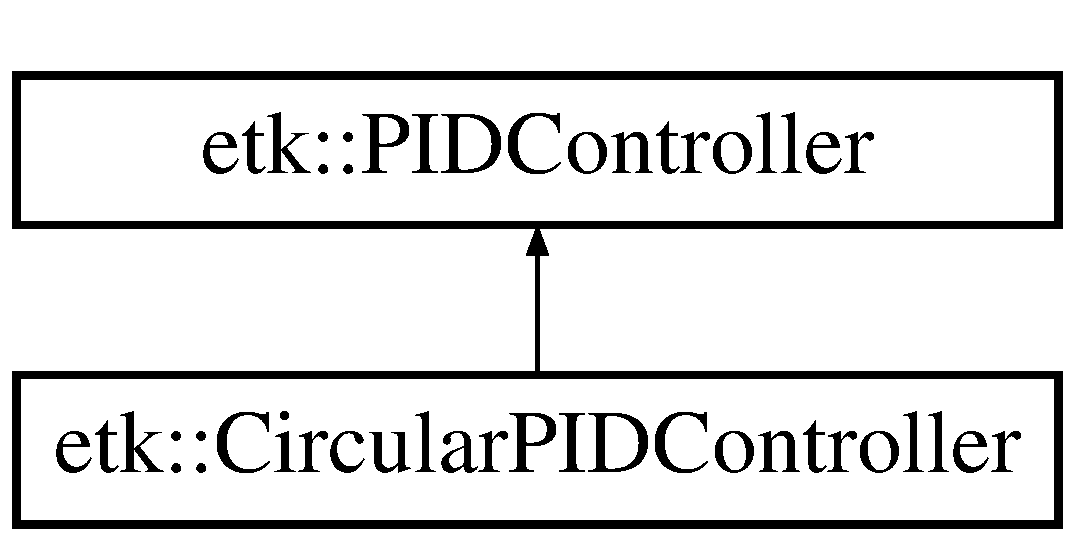
\includegraphics[height=2.000000cm]{classetk_1_1_p_i_d_controller}
\end{center}
\end{figure}
\subsection*{Public Member Functions}
\begin{DoxyCompactItemize}
\item 
real\-\_\-t \hyperlink{classetk_1_1_p_i_d_controller_af9e7e48086781b0060dd14ed6c9e135b}{step} (real\-\_\-t error, real\-\_\-t dt)
\begin{DoxyCompactList}\small\item\em Perform an interation of the P\-I\-D controller by supplying your own error value. \end{DoxyCompactList}\item 
real\-\_\-t \hyperlink{classetk_1_1_p_i_d_controller_ac17af5228b2cb3817cf72faccbdc4cd0}{step} (real\-\_\-t setpoint, real\-\_\-t measurement, real\-\_\-t dt)
\begin{DoxyCompactList}\small\item\em Perform an interation of the P\-I\-D controller using a setpoint and measurement to calculate the error. \end{DoxyCompactList}\item 
\hypertarget{classetk_1_1_p_i_d_controller_a73aecfcfe6e450178af4ec276abe8086}{void \hyperlink{classetk_1_1_p_i_d_controller_a73aecfcfe6e450178af4ec276abe8086}{set\-\_\-kp} (real\-\_\-t kp)}\label{classetk_1_1_p_i_d_controller_a73aecfcfe6e450178af4ec276abe8086}

\begin{DoxyCompactList}\small\item\em Sets the proportional gain of the controller. \end{DoxyCompactList}\item 
\hypertarget{classetk_1_1_p_i_d_controller_a6112e212a37ed7a2950c62f558cc489c}{void \hyperlink{classetk_1_1_p_i_d_controller_a6112e212a37ed7a2950c62f558cc489c}{set\-\_\-ki} (real\-\_\-t ki)}\label{classetk_1_1_p_i_d_controller_a6112e212a37ed7a2950c62f558cc489c}

\begin{DoxyCompactList}\small\item\em Sets the integral gain of the controller. This functional also scales the integral so that there is no large disturbance to the output. \end{DoxyCompactList}\item 
\hypertarget{classetk_1_1_p_i_d_controller_a1e5de9c92d5ceb2d1a94c87e1f118631}{void \hyperlink{classetk_1_1_p_i_d_controller_a1e5de9c92d5ceb2d1a94c87e1f118631}{set\-\_\-kd} (real\-\_\-t kd)}\label{classetk_1_1_p_i_d_controller_a1e5de9c92d5ceb2d1a94c87e1f118631}

\begin{DoxyCompactList}\small\item\em Sets the derivative gain. \end{DoxyCompactList}\item 
\hypertarget{classetk_1_1_p_i_d_controller_a438f51c529a8171b3c18d564461add26}{real\-\_\-t {\bfseries get\-\_\-kp} ()}\label{classetk_1_1_p_i_d_controller_a438f51c529a8171b3c18d564461add26}

\item 
\hypertarget{classetk_1_1_p_i_d_controller_af6d39b029c8ad621acbabf36425268dd}{real\-\_\-t {\bfseries get\-\_\-ki} ()}\label{classetk_1_1_p_i_d_controller_af6d39b029c8ad621acbabf36425268dd}

\item 
\hypertarget{classetk_1_1_p_i_d_controller_a69fd9c40b85ddba301a7acc5ba658255}{real\-\_\-t {\bfseries get\-\_\-kd} ()}\label{classetk_1_1_p_i_d_controller_a69fd9c40b85ddba301a7acc5ba658255}

\item 
\hypertarget{classetk_1_1_p_i_d_controller_a02af725f99fb1e0131674f7602fd635e}{void \hyperlink{classetk_1_1_p_i_d_controller_a02af725f99fb1e0131674f7602fd635e}{reset\-\_\-integral} ()}\label{classetk_1_1_p_i_d_controller_a02af725f99fb1e0131674f7602fd635e}

\begin{DoxyCompactList}\small\item\em Sets the integral to zero. \end{DoxyCompactList}\item 
\hypertarget{classetk_1_1_p_i_d_controller_a19b27067a3b56846245b8ca14919e98b}{void \hyperlink{classetk_1_1_p_i_d_controller_a19b27067a3b56846245b8ca14919e98b}{set\-\_\-max\-\_\-integral} (real\-\_\-t imax)}\label{classetk_1_1_p_i_d_controller_a19b27067a3b56846245b8ca14919e98b}

\begin{DoxyCompactList}\small\item\em Sets a maximum size for the integral. This can help prevent integral wind up. \end{DoxyCompactList}\item 
\hypertarget{classetk_1_1_p_i_d_controller_a023f411018741e4c1265284de78b5f53}{void \hyperlink{classetk_1_1_p_i_d_controller_a023f411018741e4c1265284de78b5f53}{set\-\_\-derivative\-\_\-filter\-\_\-gain} (real\-\_\-t g)}\label{classetk_1_1_p_i_d_controller_a023f411018741e4c1265284de78b5f53}

\begin{DoxyCompactList}\small\item\em Sets the derivative filter gain. The derivative filter is an \hyperlink{classetk_1_1_expo_moving_avg}{Expo\-Moving\-Avg} filter. \end{DoxyCompactList}\item 
\hypertarget{classetk_1_1_p_i_d_controller_a25ba04e64f94802a65bc464e3b364595}{real\-\_\-t \hyperlink{classetk_1_1_p_i_d_controller_a25ba04e64f94802a65bc464e3b364595}{get\-\_\-integral} ()}\label{classetk_1_1_p_i_d_controller_a25ba04e64f94802a65bc464e3b364595}

\begin{DoxyCompactList}\small\item\em Returns the integral value. \end{DoxyCompactList}\item 
\hypertarget{classetk_1_1_p_i_d_controller_acb730031d516c2324ea5f735ae5b438d}{void \hyperlink{classetk_1_1_p_i_d_controller_acb730031d516c2324ea5f735ae5b438d}{set\-\_\-integral} (real\-\_\-t integ)}\label{classetk_1_1_p_i_d_controller_acb730031d516c2324ea5f735ae5b438d}

\begin{DoxyCompactList}\small\item\em Sets the integral value. U\-S\-E W\-I\-T\-H C\-A\-U\-T\-I\-O\-N. Suddenly changing the integral will suddenly change the output. \end{DoxyCompactList}\end{DoxyCompactItemize}
\subsection*{Protected Attributes}
\begin{DoxyCompactItemize}
\item 
\hypertarget{classetk_1_1_p_i_d_controller_a8e71515e4e16b112002214af79c11a1a}{real\-\_\-t {\bfseries integral}}\label{classetk_1_1_p_i_d_controller_a8e71515e4e16b112002214af79c11a1a}

\item 
\hypertarget{classetk_1_1_p_i_d_controller_a19b46ebbea3393181e911e8e58fdeddb}{real\-\_\-t {\bfseries Kp}}\label{classetk_1_1_p_i_d_controller_a19b46ebbea3393181e911e8e58fdeddb}

\item 
\hypertarget{classetk_1_1_p_i_d_controller_aa8250f45b88af74887e8e35074a558d5}{real\-\_\-t {\bfseries Ki}}\label{classetk_1_1_p_i_d_controller_aa8250f45b88af74887e8e35074a558d5}

\item 
\hypertarget{classetk_1_1_p_i_d_controller_a24c0abfcf440a7198c70fa7591299daf}{real\-\_\-t {\bfseries Kd}}\label{classetk_1_1_p_i_d_controller_a24c0abfcf440a7198c70fa7591299daf}

\item 
\hypertarget{classetk_1_1_p_i_d_controller_a5ad94c73ac49a5ab7dc0792d0856319c}{real\-\_\-t {\bfseries integral\-\_\-constraint}}\label{classetk_1_1_p_i_d_controller_a5ad94c73ac49a5ab7dc0792d0856319c}

\item 
\hypertarget{classetk_1_1_p_i_d_controller_a0c791c5663de648256850318f89b70c1}{\hyperlink{classetk_1_1_expo_moving_avg}{Expo\-Moving\-Avg} {\bfseries der\-\_\-filter}}\label{classetk_1_1_p_i_d_controller_a0c791c5663de648256850318f89b70c1}

\item 
\hypertarget{classetk_1_1_p_i_d_controller_a52d7c2dd196497f2543965e4473e017d}{real\-\_\-t {\bfseries previous\-\_\-error}}\label{classetk_1_1_p_i_d_controller_a52d7c2dd196497f2543965e4473e017d}

\end{DoxyCompactItemize}


\subsection{Detailed Description}
A generic \hyperlink{classetk_1_1_p_i_d_controller}{P\-I\-D\-Controller}. \href{https://en.wikipedia.org/wiki/PID_controller}{\tt https\-://en.\-wikipedia.\-org/wiki/\-P\-I\-D\-\_\-controller}. 

\subsection{Member Function Documentation}
\hypertarget{classetk_1_1_p_i_d_controller_af9e7e48086781b0060dd14ed6c9e135b}{\index{etk\-::\-P\-I\-D\-Controller@{etk\-::\-P\-I\-D\-Controller}!step@{step}}
\index{step@{step}!etk::PIDController@{etk\-::\-P\-I\-D\-Controller}}
\subsubsection[{step}]{\setlength{\rightskip}{0pt plus 5cm}real\-\_\-t etk\-::\-P\-I\-D\-Controller\-::step (
\begin{DoxyParamCaption}
\item[{real\-\_\-t}]{error, }
\item[{real\-\_\-t}]{dt}
\end{DoxyParamCaption}
)}}\label{classetk_1_1_p_i_d_controller_af9e7e48086781b0060dd14ed6c9e135b}


Perform an interation of the P\-I\-D controller by supplying your own error value. 

\begin{DoxyItemize}
\item error Some pre-\/calculated error value. \item dt \hyperlink{classetk_1_1_time}{Time} period since the last iteration. \begin{DoxyReturn}{Returns}
Control output. 
\end{DoxyReturn}
\end{DoxyItemize}
\hypertarget{classetk_1_1_p_i_d_controller_ac17af5228b2cb3817cf72faccbdc4cd0}{\index{etk\-::\-P\-I\-D\-Controller@{etk\-::\-P\-I\-D\-Controller}!step@{step}}
\index{step@{step}!etk::PIDController@{etk\-::\-P\-I\-D\-Controller}}
\subsubsection[{step}]{\setlength{\rightskip}{0pt plus 5cm}real\-\_\-t etk\-::\-P\-I\-D\-Controller\-::step (
\begin{DoxyParamCaption}
\item[{real\-\_\-t}]{setpoint, }
\item[{real\-\_\-t}]{measurement, }
\item[{real\-\_\-t}]{dt}
\end{DoxyParamCaption}
)}}\label{classetk_1_1_p_i_d_controller_ac17af5228b2cb3817cf72faccbdc4cd0}


Perform an interation of the P\-I\-D controller using a setpoint and measurement to calculate the error. 

\begin{DoxyItemize}
\item setpoint The setpoint \item measurement The measurement \item dt \hyperlink{classetk_1_1_time}{Time} period since the last iteration. \begin{DoxyReturn}{Returns}
Control output. 
\end{DoxyReturn}
\end{DoxyItemize}


The documentation for this class was generated from the following file\-:\begin{DoxyCompactItemize}
\item 
inc/etk/pid.\-h\end{DoxyCompactItemize}

\input{classetk_1_1_evo_pid_1_1_p_i_d_gain}
\input{classetk_1_1_p_i_d_rater}
\input{classetk_1_1_pool_ptr}
\hypertarget{classetk_1_1_quaternion}{\section{etk\-:\-:Quaternion Class Reference}
\label{classetk_1_1_quaternion}\index{etk\-::\-Quaternion@{etk\-::\-Quaternion}}
}


{\ttfamily \#include $<$quaternion.\-h$>$}

\subsection*{Public Member Functions}
\begin{DoxyCompactItemize}
\item 
\hyperlink{classetk_1_1_quaternion_a84e5df2bfc9c0a28324f435bc7e982e9}{Quaternion} ()
\item 
\hyperlink{classetk_1_1_quaternion_ab87d30ca3035f35d0b2398040faa433c}{Quaternion} (float iw, float ix, float iy, float iz)
\item 
\hyperlink{classetk_1_1_quaternion_af9f52e0be9887cf14c9d84c518118812}{Quaternion} (float \hyperlink{classetk_1_1_quaternion_ae8087566ada295e00a13be97a090acc3}{w}, \hyperlink{classetk_1_1_vector}{Vector}$<$ 3 $>$ vec)
\item 
\hyperlink{classetk_1_1_quaternion_a284ec056776c41d681670a76b49eaeac}{Quaternion} (\hyperlink{classetk_1_1_vector}{Vector}$<$ 4 $>$ v)
\item 
\hyperlink{classetk_1_1_vector}{Vector}$<$ 4 $>$ \hyperlink{classetk_1_1_quaternion_a7c1a3035f2cbf11cb30a29bd1516b801}{to\-\_\-vector} ()
\item 
void \hyperlink{classetk_1_1_quaternion_ae39c916d1534200ec39f04b036aeb97c}{set\-\_\-vector} (\hyperlink{classetk_1_1_vector}{Vector}$<$ 3 $>$ v)
\item 
float \& \hyperlink{classetk_1_1_quaternion_ae8087566ada295e00a13be97a090acc3}{w} ()
\item 
float \& \hyperlink{classetk_1_1_quaternion_ad76e562f566d259c2c9f1ec22d31c1b1}{x} ()
\item 
float \& \hyperlink{classetk_1_1_quaternion_a15f04dac1d1b9d0ae20560e8872d09d7}{y} ()
\item 
float \& \hyperlink{classetk_1_1_quaternion_ab0ec0b04e80256bbd09dccd3612b0a74}{z} ()
\item 
float \hyperlink{classetk_1_1_quaternion_a858bc7b7679991c4184f787e90088374}{magnitude} ()
\item 
void \hyperlink{classetk_1_1_quaternion_a2fea07c80f64acf916c4141068d4dc4d}{normalize} ()
\item 
\hyperlink{classetk_1_1_quaternion}{Quaternion} \hyperlink{classetk_1_1_quaternion_ad5fa5e5d2edbcee852480e63053daf80}{conjugate} ()
\item 
void \hyperlink{classetk_1_1_quaternion_ae191a92873826ad1de7495810a0ed1a9}{from\-Euler} (\hyperlink{classetk_1_1_vector}{Vector}$<$ 3 $>$ euler)
\item 
void \hyperlink{classetk_1_1_quaternion_a682f23ae7b2d38e78660456d10937306}{from\-Axis\-Angle} (\hyperlink{classetk_1_1_vector}{Vector}$<$ 3 $>$ axis, float theta)
\item 
void \hyperlink{classetk_1_1_quaternion_adc1333e656e74c33f3f1169a32614fb0}{to\-Axis\-Angle} (\hyperlink{classetk_1_1_vector}{Vector}$<$ 3 $>$ \&axis, float \&angle)
\item 
void \hyperlink{classetk_1_1_quaternion_a6dd99f266dfb3338e9fa3a61fac8b046}{from\-Matrix} (\hyperlink{classetk_1_1_matrix}{Matrix}$<$ 3, 3 $>$ m)
\item 
\hyperlink{classetk_1_1_matrix}{Matrix}$<$ 3, 3 $>$ \hyperlink{classetk_1_1_quaternion_a3f6d295725e34994abcc00ea60e19658}{to\-Matrix} ()
\item 
\hyperlink{classetk_1_1_vector}{Vector}$<$ 3 $>$ \hyperlink{classetk_1_1_quaternion_a81ad691231786ab3a13157bfbc6de1ec}{to\-Euler} ()
\item 
\hyperlink{classetk_1_1_vector}{Vector}$<$ 3 $>$ \hyperlink{classetk_1_1_quaternion_a594a9d43225c192559670a6038cbb136}{to\-Angular\-Velocity} (float dt)
\item 
void \hyperlink{classetk_1_1_quaternion_a5cb0bc620fc02826964bf53ddde65cb7}{from\-Angular\-Velocity} (\hyperlink{classetk_1_1_vector}{Vector}$<$ 3 $>$ \hyperlink{classetk_1_1_quaternion_ae8087566ada295e00a13be97a090acc3}{w}, float dt)
\item 
\hyperlink{classetk_1_1_vector}{Vector}$<$ 3 $>$ \hyperlink{classetk_1_1_quaternion_a8c5bdf49977cb3c9c9e3189b75b224c2}{rotate\-Vector} (\hyperlink{classetk_1_1_vector}{Vector}$<$ 2 $>$ v)
\item 
\hyperlink{classetk_1_1_vector}{Vector}$<$ 3 $>$ \hyperlink{classetk_1_1_quaternion_afa4cab588a1fdfa2c2ca0e2f60473063}{rotate\-Vector} (\hyperlink{classetk_1_1_vector}{Vector}$<$ 3 $>$ v)
\item 
\hyperlink{classetk_1_1_quaternion}{Quaternion} \hyperlink{classetk_1_1_quaternion_acfd5de59138eb00b43d5c2633152d72d}{operator$\ast$} (\hyperlink{classetk_1_1_quaternion}{Quaternion} q)
\item 
\hyperlink{classetk_1_1_vector}{Vector}$<$ 3 $>$ \hyperlink{classetk_1_1_quaternion_a7ed0b672fabb560607b8260429b3e4af}{operator$\ast$} (\hyperlink{classetk_1_1_vector}{Vector}$<$ 3 $>$ v)
\item 
\hyperlink{classetk_1_1_quaternion}{Quaternion} \hyperlink{classetk_1_1_quaternion_a661853921fda0ca0cd44f52bea9196bf}{operator+} (\hyperlink{classetk_1_1_quaternion}{Quaternion} q)
\item 
\hyperlink{classetk_1_1_quaternion}{Quaternion} \hyperlink{classetk_1_1_quaternion_a5294305248643853bc3258f24930cece}{operator-\/} (\hyperlink{classetk_1_1_quaternion}{Quaternion} q)
\item 
\hyperlink{classetk_1_1_quaternion}{Quaternion} \hyperlink{classetk_1_1_quaternion_a1ea27ca901b892ace102c2a32108ecb7}{operator/} (float scalar)
\item 
\hyperlink{classetk_1_1_quaternion}{Quaternion} \hyperlink{classetk_1_1_quaternion_a9e68d3c912cc53ef6f8a5224c4571e86}{operator$\ast$} (float scalar)
\item 
\hyperlink{classetk_1_1_quaternion}{Quaternion} \hyperlink{classetk_1_1_quaternion_a16bc6ba21e171da1afb1e2fa2b8692e2}{scale} (float scalar)
\end{DoxyCompactItemize}


\subsection{Constructor \& Destructor Documentation}
\hypertarget{classetk_1_1_quaternion_a84e5df2bfc9c0a28324f435bc7e982e9}{\index{etk\-::\-Quaternion@{etk\-::\-Quaternion}!Quaternion@{Quaternion}}
\index{Quaternion@{Quaternion}!etk::Quaternion@{etk\-::\-Quaternion}}
\subsubsection[{Quaternion}]{\setlength{\rightskip}{0pt plus 5cm}etk\-::\-Quaternion\-::\-Quaternion (
\begin{DoxyParamCaption}
{}
\end{DoxyParamCaption}
)\hspace{0.3cm}{\ttfamily [inline]}}}\label{classetk_1_1_quaternion_a84e5df2bfc9c0a28324f435bc7e982e9}
\hypertarget{classetk_1_1_quaternion_ab87d30ca3035f35d0b2398040faa433c}{\index{etk\-::\-Quaternion@{etk\-::\-Quaternion}!Quaternion@{Quaternion}}
\index{Quaternion@{Quaternion}!etk::Quaternion@{etk\-::\-Quaternion}}
\subsubsection[{Quaternion}]{\setlength{\rightskip}{0pt plus 5cm}etk\-::\-Quaternion\-::\-Quaternion (
\begin{DoxyParamCaption}
\item[{float}]{iw, }
\item[{float}]{ix, }
\item[{float}]{iy, }
\item[{float}]{iz}
\end{DoxyParamCaption}
)\hspace{0.3cm}{\ttfamily [inline]}}}\label{classetk_1_1_quaternion_ab87d30ca3035f35d0b2398040faa433c}
\hypertarget{classetk_1_1_quaternion_af9f52e0be9887cf14c9d84c518118812}{\index{etk\-::\-Quaternion@{etk\-::\-Quaternion}!Quaternion@{Quaternion}}
\index{Quaternion@{Quaternion}!etk::Quaternion@{etk\-::\-Quaternion}}
\subsubsection[{Quaternion}]{\setlength{\rightskip}{0pt plus 5cm}etk\-::\-Quaternion\-::\-Quaternion (
\begin{DoxyParamCaption}
\item[{float}]{w, }
\item[{{\bf Vector}$<$ 3 $>$}]{vec}
\end{DoxyParamCaption}
)\hspace{0.3cm}{\ttfamily [inline]}}}\label{classetk_1_1_quaternion_af9f52e0be9887cf14c9d84c518118812}
\hypertarget{classetk_1_1_quaternion_a284ec056776c41d681670a76b49eaeac}{\index{etk\-::\-Quaternion@{etk\-::\-Quaternion}!Quaternion@{Quaternion}}
\index{Quaternion@{Quaternion}!etk::Quaternion@{etk\-::\-Quaternion}}
\subsubsection[{Quaternion}]{\setlength{\rightskip}{0pt plus 5cm}etk\-::\-Quaternion\-::\-Quaternion (
\begin{DoxyParamCaption}
\item[{{\bf Vector}$<$ 4 $>$}]{v}
\end{DoxyParamCaption}
)\hspace{0.3cm}{\ttfamily [inline]}}}\label{classetk_1_1_quaternion_a284ec056776c41d681670a76b49eaeac}


\subsection{Member Function Documentation}
\hypertarget{classetk_1_1_quaternion_ad5fa5e5d2edbcee852480e63053daf80}{\index{etk\-::\-Quaternion@{etk\-::\-Quaternion}!conjugate@{conjugate}}
\index{conjugate@{conjugate}!etk::Quaternion@{etk\-::\-Quaternion}}
\subsubsection[{conjugate}]{\setlength{\rightskip}{0pt plus 5cm}{\bf Quaternion} etk\-::\-Quaternion\-::conjugate (
\begin{DoxyParamCaption}
{}
\end{DoxyParamCaption}
)\hspace{0.3cm}{\ttfamily [inline]}}}\label{classetk_1_1_quaternion_ad5fa5e5d2edbcee852480e63053daf80}
\hypertarget{classetk_1_1_quaternion_a5cb0bc620fc02826964bf53ddde65cb7}{\index{etk\-::\-Quaternion@{etk\-::\-Quaternion}!from\-Angular\-Velocity@{from\-Angular\-Velocity}}
\index{from\-Angular\-Velocity@{from\-Angular\-Velocity}!etk::Quaternion@{etk\-::\-Quaternion}}
\subsubsection[{from\-Angular\-Velocity}]{\setlength{\rightskip}{0pt plus 5cm}void etk\-::\-Quaternion\-::from\-Angular\-Velocity (
\begin{DoxyParamCaption}
\item[{{\bf Vector}$<$ 3 $>$}]{w, }
\item[{float}]{dt}
\end{DoxyParamCaption}
)\hspace{0.3cm}{\ttfamily [inline]}}}\label{classetk_1_1_quaternion_a5cb0bc620fc02826964bf53ddde65cb7}
\hypertarget{classetk_1_1_quaternion_a682f23ae7b2d38e78660456d10937306}{\index{etk\-::\-Quaternion@{etk\-::\-Quaternion}!from\-Axis\-Angle@{from\-Axis\-Angle}}
\index{from\-Axis\-Angle@{from\-Axis\-Angle}!etk::Quaternion@{etk\-::\-Quaternion}}
\subsubsection[{from\-Axis\-Angle}]{\setlength{\rightskip}{0pt plus 5cm}void etk\-::\-Quaternion\-::from\-Axis\-Angle (
\begin{DoxyParamCaption}
\item[{{\bf Vector}$<$ 3 $>$}]{axis, }
\item[{float}]{theta}
\end{DoxyParamCaption}
)\hspace{0.3cm}{\ttfamily [inline]}}}\label{classetk_1_1_quaternion_a682f23ae7b2d38e78660456d10937306}
\hypertarget{classetk_1_1_quaternion_ae191a92873826ad1de7495810a0ed1a9}{\index{etk\-::\-Quaternion@{etk\-::\-Quaternion}!from\-Euler@{from\-Euler}}
\index{from\-Euler@{from\-Euler}!etk::Quaternion@{etk\-::\-Quaternion}}
\subsubsection[{from\-Euler}]{\setlength{\rightskip}{0pt plus 5cm}void etk\-::\-Quaternion\-::from\-Euler (
\begin{DoxyParamCaption}
\item[{{\bf Vector}$<$ 3 $>$}]{euler}
\end{DoxyParamCaption}
)\hspace{0.3cm}{\ttfamily [inline]}}}\label{classetk_1_1_quaternion_ae191a92873826ad1de7495810a0ed1a9}
\hypertarget{classetk_1_1_quaternion_a6dd99f266dfb3338e9fa3a61fac8b046}{\index{etk\-::\-Quaternion@{etk\-::\-Quaternion}!from\-Matrix@{from\-Matrix}}
\index{from\-Matrix@{from\-Matrix}!etk::Quaternion@{etk\-::\-Quaternion}}
\subsubsection[{from\-Matrix}]{\setlength{\rightskip}{0pt plus 5cm}void etk\-::\-Quaternion\-::from\-Matrix (
\begin{DoxyParamCaption}
\item[{{\bf Matrix}$<$ 3, 3 $>$}]{m}
\end{DoxyParamCaption}
)\hspace{0.3cm}{\ttfamily [inline]}}}\label{classetk_1_1_quaternion_a6dd99f266dfb3338e9fa3a61fac8b046}
\hypertarget{classetk_1_1_quaternion_a858bc7b7679991c4184f787e90088374}{\index{etk\-::\-Quaternion@{etk\-::\-Quaternion}!magnitude@{magnitude}}
\index{magnitude@{magnitude}!etk::Quaternion@{etk\-::\-Quaternion}}
\subsubsection[{magnitude}]{\setlength{\rightskip}{0pt plus 5cm}float etk\-::\-Quaternion\-::magnitude (
\begin{DoxyParamCaption}
{}
\end{DoxyParamCaption}
)\hspace{0.3cm}{\ttfamily [inline]}}}\label{classetk_1_1_quaternion_a858bc7b7679991c4184f787e90088374}
\hypertarget{classetk_1_1_quaternion_a2fea07c80f64acf916c4141068d4dc4d}{\index{etk\-::\-Quaternion@{etk\-::\-Quaternion}!normalize@{normalize}}
\index{normalize@{normalize}!etk::Quaternion@{etk\-::\-Quaternion}}
\subsubsection[{normalize}]{\setlength{\rightskip}{0pt plus 5cm}void etk\-::\-Quaternion\-::normalize (
\begin{DoxyParamCaption}
{}
\end{DoxyParamCaption}
)\hspace{0.3cm}{\ttfamily [inline]}}}\label{classetk_1_1_quaternion_a2fea07c80f64acf916c4141068d4dc4d}
\hypertarget{classetk_1_1_quaternion_acfd5de59138eb00b43d5c2633152d72d}{\index{etk\-::\-Quaternion@{etk\-::\-Quaternion}!operator$\ast$@{operator$\ast$}}
\index{operator$\ast$@{operator$\ast$}!etk::Quaternion@{etk\-::\-Quaternion}}
\subsubsection[{operator$\ast$}]{\setlength{\rightskip}{0pt plus 5cm}{\bf Quaternion} etk\-::\-Quaternion\-::operator$\ast$ (
\begin{DoxyParamCaption}
\item[{{\bf Quaternion}}]{q}
\end{DoxyParamCaption}
)\hspace{0.3cm}{\ttfamily [inline]}}}\label{classetk_1_1_quaternion_acfd5de59138eb00b43d5c2633152d72d}
\hypertarget{classetk_1_1_quaternion_a7ed0b672fabb560607b8260429b3e4af}{\index{etk\-::\-Quaternion@{etk\-::\-Quaternion}!operator$\ast$@{operator$\ast$}}
\index{operator$\ast$@{operator$\ast$}!etk::Quaternion@{etk\-::\-Quaternion}}
\subsubsection[{operator$\ast$}]{\setlength{\rightskip}{0pt plus 5cm}{\bf Vector}$<$3$>$ etk\-::\-Quaternion\-::operator$\ast$ (
\begin{DoxyParamCaption}
\item[{{\bf Vector}$<$ 3 $>$}]{v}
\end{DoxyParamCaption}
)\hspace{0.3cm}{\ttfamily [inline]}}}\label{classetk_1_1_quaternion_a7ed0b672fabb560607b8260429b3e4af}
\hypertarget{classetk_1_1_quaternion_a9e68d3c912cc53ef6f8a5224c4571e86}{\index{etk\-::\-Quaternion@{etk\-::\-Quaternion}!operator$\ast$@{operator$\ast$}}
\index{operator$\ast$@{operator$\ast$}!etk::Quaternion@{etk\-::\-Quaternion}}
\subsubsection[{operator$\ast$}]{\setlength{\rightskip}{0pt plus 5cm}{\bf Quaternion} etk\-::\-Quaternion\-::operator$\ast$ (
\begin{DoxyParamCaption}
\item[{float}]{scalar}
\end{DoxyParamCaption}
)\hspace{0.3cm}{\ttfamily [inline]}}}\label{classetk_1_1_quaternion_a9e68d3c912cc53ef6f8a5224c4571e86}
\hypertarget{classetk_1_1_quaternion_a661853921fda0ca0cd44f52bea9196bf}{\index{etk\-::\-Quaternion@{etk\-::\-Quaternion}!operator+@{operator+}}
\index{operator+@{operator+}!etk::Quaternion@{etk\-::\-Quaternion}}
\subsubsection[{operator+}]{\setlength{\rightskip}{0pt plus 5cm}{\bf Quaternion} etk\-::\-Quaternion\-::operator+ (
\begin{DoxyParamCaption}
\item[{{\bf Quaternion}}]{q}
\end{DoxyParamCaption}
)\hspace{0.3cm}{\ttfamily [inline]}}}\label{classetk_1_1_quaternion_a661853921fda0ca0cd44f52bea9196bf}
\hypertarget{classetk_1_1_quaternion_a5294305248643853bc3258f24930cece}{\index{etk\-::\-Quaternion@{etk\-::\-Quaternion}!operator-\/@{operator-\/}}
\index{operator-\/@{operator-\/}!etk::Quaternion@{etk\-::\-Quaternion}}
\subsubsection[{operator-\/}]{\setlength{\rightskip}{0pt plus 5cm}{\bf Quaternion} etk\-::\-Quaternion\-::operator-\/ (
\begin{DoxyParamCaption}
\item[{{\bf Quaternion}}]{q}
\end{DoxyParamCaption}
)\hspace{0.3cm}{\ttfamily [inline]}}}\label{classetk_1_1_quaternion_a5294305248643853bc3258f24930cece}
\hypertarget{classetk_1_1_quaternion_a1ea27ca901b892ace102c2a32108ecb7}{\index{etk\-::\-Quaternion@{etk\-::\-Quaternion}!operator/@{operator/}}
\index{operator/@{operator/}!etk::Quaternion@{etk\-::\-Quaternion}}
\subsubsection[{operator/}]{\setlength{\rightskip}{0pt plus 5cm}{\bf Quaternion} etk\-::\-Quaternion\-::operator/ (
\begin{DoxyParamCaption}
\item[{float}]{scalar}
\end{DoxyParamCaption}
)\hspace{0.3cm}{\ttfamily [inline]}}}\label{classetk_1_1_quaternion_a1ea27ca901b892ace102c2a32108ecb7}
\hypertarget{classetk_1_1_quaternion_a8c5bdf49977cb3c9c9e3189b75b224c2}{\index{etk\-::\-Quaternion@{etk\-::\-Quaternion}!rotate\-Vector@{rotate\-Vector}}
\index{rotate\-Vector@{rotate\-Vector}!etk::Quaternion@{etk\-::\-Quaternion}}
\subsubsection[{rotate\-Vector}]{\setlength{\rightskip}{0pt plus 5cm}{\bf Vector}$<$3$>$ etk\-::\-Quaternion\-::rotate\-Vector (
\begin{DoxyParamCaption}
\item[{{\bf Vector}$<$ 2 $>$}]{v}
\end{DoxyParamCaption}
)\hspace{0.3cm}{\ttfamily [inline]}}}\label{classetk_1_1_quaternion_a8c5bdf49977cb3c9c9e3189b75b224c2}
\hypertarget{classetk_1_1_quaternion_afa4cab588a1fdfa2c2ca0e2f60473063}{\index{etk\-::\-Quaternion@{etk\-::\-Quaternion}!rotate\-Vector@{rotate\-Vector}}
\index{rotate\-Vector@{rotate\-Vector}!etk::Quaternion@{etk\-::\-Quaternion}}
\subsubsection[{rotate\-Vector}]{\setlength{\rightskip}{0pt plus 5cm}{\bf Vector}$<$3$>$ etk\-::\-Quaternion\-::rotate\-Vector (
\begin{DoxyParamCaption}
\item[{{\bf Vector}$<$ 3 $>$}]{v}
\end{DoxyParamCaption}
)\hspace{0.3cm}{\ttfamily [inline]}}}\label{classetk_1_1_quaternion_afa4cab588a1fdfa2c2ca0e2f60473063}
\hypertarget{classetk_1_1_quaternion_a16bc6ba21e171da1afb1e2fa2b8692e2}{\index{etk\-::\-Quaternion@{etk\-::\-Quaternion}!scale@{scale}}
\index{scale@{scale}!etk::Quaternion@{etk\-::\-Quaternion}}
\subsubsection[{scale}]{\setlength{\rightskip}{0pt plus 5cm}{\bf Quaternion} etk\-::\-Quaternion\-::scale (
\begin{DoxyParamCaption}
\item[{float}]{scalar}
\end{DoxyParamCaption}
)\hspace{0.3cm}{\ttfamily [inline]}}}\label{classetk_1_1_quaternion_a16bc6ba21e171da1afb1e2fa2b8692e2}
\hypertarget{classetk_1_1_quaternion_ae39c916d1534200ec39f04b036aeb97c}{\index{etk\-::\-Quaternion@{etk\-::\-Quaternion}!set\-\_\-vector@{set\-\_\-vector}}
\index{set\-\_\-vector@{set\-\_\-vector}!etk::Quaternion@{etk\-::\-Quaternion}}
\subsubsection[{set\-\_\-vector}]{\setlength{\rightskip}{0pt plus 5cm}void etk\-::\-Quaternion\-::set\-\_\-vector (
\begin{DoxyParamCaption}
\item[{{\bf Vector}$<$ 3 $>$}]{v}
\end{DoxyParamCaption}
)\hspace{0.3cm}{\ttfamily [inline]}}}\label{classetk_1_1_quaternion_ae39c916d1534200ec39f04b036aeb97c}
\hypertarget{classetk_1_1_quaternion_a7c1a3035f2cbf11cb30a29bd1516b801}{\index{etk\-::\-Quaternion@{etk\-::\-Quaternion}!to\-\_\-vector@{to\-\_\-vector}}
\index{to\-\_\-vector@{to\-\_\-vector}!etk::Quaternion@{etk\-::\-Quaternion}}
\subsubsection[{to\-\_\-vector}]{\setlength{\rightskip}{0pt plus 5cm}{\bf Vector}$<$4$>$ etk\-::\-Quaternion\-::to\-\_\-vector (
\begin{DoxyParamCaption}
{}
\end{DoxyParamCaption}
)\hspace{0.3cm}{\ttfamily [inline]}}}\label{classetk_1_1_quaternion_a7c1a3035f2cbf11cb30a29bd1516b801}
\hypertarget{classetk_1_1_quaternion_a594a9d43225c192559670a6038cbb136}{\index{etk\-::\-Quaternion@{etk\-::\-Quaternion}!to\-Angular\-Velocity@{to\-Angular\-Velocity}}
\index{to\-Angular\-Velocity@{to\-Angular\-Velocity}!etk::Quaternion@{etk\-::\-Quaternion}}
\subsubsection[{to\-Angular\-Velocity}]{\setlength{\rightskip}{0pt plus 5cm}{\bf Vector}$<$3$>$ etk\-::\-Quaternion\-::to\-Angular\-Velocity (
\begin{DoxyParamCaption}
\item[{float}]{dt}
\end{DoxyParamCaption}
)\hspace{0.3cm}{\ttfamily [inline]}}}\label{classetk_1_1_quaternion_a594a9d43225c192559670a6038cbb136}
\hypertarget{classetk_1_1_quaternion_adc1333e656e74c33f3f1169a32614fb0}{\index{etk\-::\-Quaternion@{etk\-::\-Quaternion}!to\-Axis\-Angle@{to\-Axis\-Angle}}
\index{to\-Axis\-Angle@{to\-Axis\-Angle}!etk::Quaternion@{etk\-::\-Quaternion}}
\subsubsection[{to\-Axis\-Angle}]{\setlength{\rightskip}{0pt plus 5cm}void etk\-::\-Quaternion\-::to\-Axis\-Angle (
\begin{DoxyParamCaption}
\item[{{\bf Vector}$<$ 3 $>$ \&}]{axis, }
\item[{float \&}]{angle}
\end{DoxyParamCaption}
)\hspace{0.3cm}{\ttfamily [inline]}}}\label{classetk_1_1_quaternion_adc1333e656e74c33f3f1169a32614fb0}
\hypertarget{classetk_1_1_quaternion_a81ad691231786ab3a13157bfbc6de1ec}{\index{etk\-::\-Quaternion@{etk\-::\-Quaternion}!to\-Euler@{to\-Euler}}
\index{to\-Euler@{to\-Euler}!etk::Quaternion@{etk\-::\-Quaternion}}
\subsubsection[{to\-Euler}]{\setlength{\rightskip}{0pt plus 5cm}{\bf Vector}$<$3$>$ etk\-::\-Quaternion\-::to\-Euler (
\begin{DoxyParamCaption}
{}
\end{DoxyParamCaption}
)\hspace{0.3cm}{\ttfamily [inline]}}}\label{classetk_1_1_quaternion_a81ad691231786ab3a13157bfbc6de1ec}
\hypertarget{classetk_1_1_quaternion_a3f6d295725e34994abcc00ea60e19658}{\index{etk\-::\-Quaternion@{etk\-::\-Quaternion}!to\-Matrix@{to\-Matrix}}
\index{to\-Matrix@{to\-Matrix}!etk::Quaternion@{etk\-::\-Quaternion}}
\subsubsection[{to\-Matrix}]{\setlength{\rightskip}{0pt plus 5cm}{\bf Matrix}$<$3, 3$>$ etk\-::\-Quaternion\-::to\-Matrix (
\begin{DoxyParamCaption}
{}
\end{DoxyParamCaption}
)\hspace{0.3cm}{\ttfamily [inline]}}}\label{classetk_1_1_quaternion_a3f6d295725e34994abcc00ea60e19658}
\hypertarget{classetk_1_1_quaternion_ae8087566ada295e00a13be97a090acc3}{\index{etk\-::\-Quaternion@{etk\-::\-Quaternion}!w@{w}}
\index{w@{w}!etk::Quaternion@{etk\-::\-Quaternion}}
\subsubsection[{w}]{\setlength{\rightskip}{0pt plus 5cm}float\& etk\-::\-Quaternion\-::w (
\begin{DoxyParamCaption}
{}
\end{DoxyParamCaption}
)\hspace{0.3cm}{\ttfamily [inline]}}}\label{classetk_1_1_quaternion_ae8087566ada295e00a13be97a090acc3}
\hypertarget{classetk_1_1_quaternion_ad76e562f566d259c2c9f1ec22d31c1b1}{\index{etk\-::\-Quaternion@{etk\-::\-Quaternion}!x@{x}}
\index{x@{x}!etk::Quaternion@{etk\-::\-Quaternion}}
\subsubsection[{x}]{\setlength{\rightskip}{0pt plus 5cm}float\& etk\-::\-Quaternion\-::x (
\begin{DoxyParamCaption}
{}
\end{DoxyParamCaption}
)\hspace{0.3cm}{\ttfamily [inline]}}}\label{classetk_1_1_quaternion_ad76e562f566d259c2c9f1ec22d31c1b1}
\hypertarget{classetk_1_1_quaternion_a15f04dac1d1b9d0ae20560e8872d09d7}{\index{etk\-::\-Quaternion@{etk\-::\-Quaternion}!y@{y}}
\index{y@{y}!etk::Quaternion@{etk\-::\-Quaternion}}
\subsubsection[{y}]{\setlength{\rightskip}{0pt plus 5cm}float\& etk\-::\-Quaternion\-::y (
\begin{DoxyParamCaption}
{}
\end{DoxyParamCaption}
)\hspace{0.3cm}{\ttfamily [inline]}}}\label{classetk_1_1_quaternion_a15f04dac1d1b9d0ae20560e8872d09d7}
\hypertarget{classetk_1_1_quaternion_ab0ec0b04e80256bbd09dccd3612b0a74}{\index{etk\-::\-Quaternion@{etk\-::\-Quaternion}!z@{z}}
\index{z@{z}!etk::Quaternion@{etk\-::\-Quaternion}}
\subsubsection[{z}]{\setlength{\rightskip}{0pt plus 5cm}float\& etk\-::\-Quaternion\-::z (
\begin{DoxyParamCaption}
{}
\end{DoxyParamCaption}
)\hspace{0.3cm}{\ttfamily [inline]}}}\label{classetk_1_1_quaternion_ab0ec0b04e80256bbd09dccd3612b0a74}


The documentation for this class was generated from the following file\-:\begin{DoxyCompactItemize}
\item 
inc/etk/\hyperlink{quaternion_8h}{quaternion.\-h}\end{DoxyCompactItemize}

\hypertarget{classetk_1_1_rate_limiter}{\section{etk\-:\-:Rate\-Limiter Class Reference}
\label{classetk_1_1_rate_limiter}\index{etk\-::\-Rate\-Limiter@{etk\-::\-Rate\-Limiter}}
}


The \hyperlink{classetk_1_1_rate_limiter}{Rate\-Limiter} limits the rate of change of a signal to a given step size.  




{\ttfamily \#include $<$filters.\-h$>$}

\subsection*{Public Member Functions}
\begin{DoxyCompactItemize}
\item 
\hypertarget{classetk_1_1_rate_limiter_a568bc9c401fa02d639715c110ca7ef51}{{\bfseries Rate\-Limiter} (real\-\_\-t max\-\_\-step, real\-\_\-t init\-\_\-val)}\label{classetk_1_1_rate_limiter_a568bc9c401fa02d639715c110ca7ef51}

\item 
\hypertarget{classetk_1_1_rate_limiter_aed6110a75c3acc8bc48fac9900c1beba}{real\-\_\-t {\bfseries step} (real\-\_\-t sample)}\label{classetk_1_1_rate_limiter_aed6110a75c3acc8bc48fac9900c1beba}

\end{DoxyCompactItemize}


\subsection{Detailed Description}
The \hyperlink{classetk_1_1_rate_limiter}{Rate\-Limiter} limits the rate of change of a signal to a given step size. 


\begin{DoxyCode}
\hyperlink{classetk_1_1_rate_limiter}{etk::RateLimiter} lim(1.0, 0.0);
\textcolor{keywordflow}{for}(\textcolor{keyword}{auto} i : \hyperlink{namespaceetk_aff39b0f367ee4d947e2e7d297ffd506b}{etk::range}(10))
    cout << lim.step(10) << \textcolor{stringliteral}{" "};
\end{DoxyCode}
 Output\-: 0,1,2,3,4,5,6,7,8,9 

The documentation for this class was generated from the following file\-:\begin{DoxyCompactItemize}
\item 
inc/etk/filters.\-h\end{DoxyCompactItemize}

\hypertarget{classetk_1_1_ring_buffer}{\section{etk\-:\-:Ring\-Buffer$<$ T, overwrite $>$ Class Template Reference}
\label{classetk_1_1_ring_buffer}\index{etk\-::\-Ring\-Buffer$<$ T, overwrite $>$@{etk\-::\-Ring\-Buffer$<$ T, overwrite $>$}}
}


Ring\-Buffers are a great way to buffer information from data streams such as U\-A\-R\-Ts. \hyperlink{classetk_1_1_ring_buffer}{Ring\-Buffer} does not allocate it's own memory, instead it requires a pointer to an array or memory region where it can store data. \par
\par
 Example.  




{\ttfamily \#include $<$ring\-\_\-buffer.\-h$>$}

\subsection*{Public Member Functions}
\begin{DoxyCompactItemize}
\item 
\hyperlink{classetk_1_1_ring_buffer_a2a6d3471b49baba47dbf58e47a6ba810}{Ring\-Buffer} (T $\ast$buffer, uint16\-\_\-t sz)
\begin{DoxyCompactList}\small\item\em The constructor. \end{DoxyCompactList}\item 
bool \hyperlink{classetk_1_1_ring_buffer_a978d9d2868965d77ecc1270d0b54707d}{is\-\_\-full} ()
\begin{DoxyCompactList}\small\item\em Returns true when the \hyperlink{classetk_1_1_ring_buffer}{Ring\-Buffer} is full. \end{DoxyCompactList}\item 
uint16\-\_\-t \hyperlink{classetk_1_1_ring_buffer_a67b70ec4c7698adcf060810c8d7756d2}{available} ()
\begin{DoxyCompactList}\small\item\em Returns the number of items queued up in the \hyperlink{classetk_1_1_ring_buffer}{Ring\-Buffer}. \end{DoxyCompactList}\item 
void \hyperlink{classetk_1_1_ring_buffer_ac17418eb9abba39351152b7d70a426ae}{put} (T b)
\begin{DoxyCompactList}\small\item\em Puts an item on to the \hyperlink{classetk_1_1_ring_buffer}{Ring\-Buffer}. \end{DoxyCompactList}\item 
void \hyperlink{classetk_1_1_ring_buffer_a251380d6c89541f0be046e6358c2307b}{increment} ()
\begin{DoxyCompactList}\small\item\em Moves the end of the ring buffer along by one position. \end{DoxyCompactList}\item 
T \hyperlink{classetk_1_1_ring_buffer_ac1327e40f6f3914156154e669076f4b8}{get} ()
\begin{DoxyCompactList}\small\item\em Removes the next item from the buffer and returns it. \end{DoxyCompactList}\item 
T \hyperlink{classetk_1_1_ring_buffer_a64f9f9a3f4ca4448a1d7365280ae4431}{peek\-\_\-ahead} (uint16\-\_\-t n=0)
\begin{DoxyCompactList}\small\item\em Returns the next item from the buffer without actually removing it. \end{DoxyCompactList}\item 
void \hyperlink{classetk_1_1_ring_buffer_a911dbba377c34fa2d20defd1a0922171}{empty} ()
\begin{DoxyCompactList}\small\item\em Makes the start and end of the ring buffer equal zero so that \hyperlink{classetk_1_1_ring_buffer_a67b70ec4c7698adcf060810c8d7756d2}{available()} return zero. \end{DoxyCompactList}\end{DoxyCompactItemize}


\subsection{Detailed Description}
\subsubsection*{template$<$class T, bool overwrite = false$>$class etk\-::\-Ring\-Buffer$<$ T, overwrite $>$}

Ring\-Buffers are a great way to buffer information from data streams such as U\-A\-R\-Ts. \hyperlink{classetk_1_1_ring_buffer}{Ring\-Buffer} does not allocate it's own memory, instead it requires a pointer to an array or memory region where it can store data. \par
\par
 Example. 


\begin{DoxyCode}
\textcolor{keywordtype}{char} usart\_buffer[128];
\hyperlink{classetk_1_1_ring_buffer}{etk::RingBuffer<char>} ringbuf(usart\_buffer, 128);

\textcolor{keywordtype}{void} usart\_isr\_hander()
\{
    ringbuf.put(USART\_READ\_BYTE());
\}

\textcolor{keywordtype}{void} foo()
\{
    \textcolor{keywordflow}{while}(ringbuf.available())
        Usart.put(ringbuf.get());
\}
\end{DoxyCode}
 
\begin{DoxyTemplParams}{Template Parameters}
{\em T} & type of object that is being buffered. For a U\-A\-R\-T this would typically be a char or uint8\-\_\-t. \\
\hline
{\em overwrite} & If overriden to true, the ring buffer will write over data when it becomes full. \\
\hline
\end{DoxyTemplParams}


\subsection{Constructor \& Destructor Documentation}
\hypertarget{classetk_1_1_ring_buffer_a2a6d3471b49baba47dbf58e47a6ba810}{\index{etk\-::\-Ring\-Buffer@{etk\-::\-Ring\-Buffer}!Ring\-Buffer@{Ring\-Buffer}}
\index{Ring\-Buffer@{Ring\-Buffer}!etk::RingBuffer@{etk\-::\-Ring\-Buffer}}
\subsubsection[{Ring\-Buffer}]{\setlength{\rightskip}{0pt plus 5cm}template$<$class T, bool overwrite = false$>$ {\bf etk\-::\-Ring\-Buffer}$<$ T, overwrite $>$\-::{\bf Ring\-Buffer} (
\begin{DoxyParamCaption}
\item[{T $\ast$}]{buffer, }
\item[{uint16\-\_\-t}]{sz}
\end{DoxyParamCaption}
)\hspace{0.3cm}{\ttfamily [inline]}}}\label{classetk_1_1_ring_buffer_a2a6d3471b49baba47dbf58e47a6ba810}


The constructor. 

\begin{DoxyItemize}
\item buffer Pointer to a writeable memory location. \item sz Maximum number of items that can be stored before the buffer is full. \end{DoxyItemize}


\subsection{Member Function Documentation}
\hypertarget{classetk_1_1_ring_buffer_a67b70ec4c7698adcf060810c8d7756d2}{\index{etk\-::\-Ring\-Buffer@{etk\-::\-Ring\-Buffer}!available@{available}}
\index{available@{available}!etk::RingBuffer@{etk\-::\-Ring\-Buffer}}
\subsubsection[{available}]{\setlength{\rightskip}{0pt plus 5cm}template$<$class T, bool overwrite = false$>$ uint16\-\_\-t {\bf etk\-::\-Ring\-Buffer}$<$ T, overwrite $>$\-::available (
\begin{DoxyParamCaption}
{}
\end{DoxyParamCaption}
)\hspace{0.3cm}{\ttfamily [inline]}}}\label{classetk_1_1_ring_buffer_a67b70ec4c7698adcf060810c8d7756d2}


Returns the number of items queued up in the \hyperlink{classetk_1_1_ring_buffer}{Ring\-Buffer}. 

\hypertarget{classetk_1_1_ring_buffer_a911dbba377c34fa2d20defd1a0922171}{\index{etk\-::\-Ring\-Buffer@{etk\-::\-Ring\-Buffer}!empty@{empty}}
\index{empty@{empty}!etk::RingBuffer@{etk\-::\-Ring\-Buffer}}
\subsubsection[{empty}]{\setlength{\rightskip}{0pt plus 5cm}template$<$class T, bool overwrite = false$>$ void {\bf etk\-::\-Ring\-Buffer}$<$ T, overwrite $>$\-::empty (
\begin{DoxyParamCaption}
{}
\end{DoxyParamCaption}
)\hspace{0.3cm}{\ttfamily [inline]}}}\label{classetk_1_1_ring_buffer_a911dbba377c34fa2d20defd1a0922171}


Makes the start and end of the ring buffer equal zero so that \hyperlink{classetk_1_1_ring_buffer_a67b70ec4c7698adcf060810c8d7756d2}{available()} return zero. 

\hypertarget{classetk_1_1_ring_buffer_ac1327e40f6f3914156154e669076f4b8}{\index{etk\-::\-Ring\-Buffer@{etk\-::\-Ring\-Buffer}!get@{get}}
\index{get@{get}!etk::RingBuffer@{etk\-::\-Ring\-Buffer}}
\subsubsection[{get}]{\setlength{\rightskip}{0pt plus 5cm}template$<$class T, bool overwrite = false$>$ T {\bf etk\-::\-Ring\-Buffer}$<$ T, overwrite $>$\-::get (
\begin{DoxyParamCaption}
{}
\end{DoxyParamCaption}
)\hspace{0.3cm}{\ttfamily [inline]}}}\label{classetk_1_1_ring_buffer_ac1327e40f6f3914156154e669076f4b8}


Removes the next item from the buffer and returns it. 

\hypertarget{classetk_1_1_ring_buffer_a251380d6c89541f0be046e6358c2307b}{\index{etk\-::\-Ring\-Buffer@{etk\-::\-Ring\-Buffer}!increment@{increment}}
\index{increment@{increment}!etk::RingBuffer@{etk\-::\-Ring\-Buffer}}
\subsubsection[{increment}]{\setlength{\rightskip}{0pt plus 5cm}template$<$class T, bool overwrite = false$>$ void {\bf etk\-::\-Ring\-Buffer}$<$ T, overwrite $>$\-::increment (
\begin{DoxyParamCaption}
{}
\end{DoxyParamCaption}
)\hspace{0.3cm}{\ttfamily [inline]}}}\label{classetk_1_1_ring_buffer_a251380d6c89541f0be046e6358c2307b}


Moves the end of the ring buffer along by one position. 

\hypertarget{classetk_1_1_ring_buffer_a978d9d2868965d77ecc1270d0b54707d}{\index{etk\-::\-Ring\-Buffer@{etk\-::\-Ring\-Buffer}!is\-\_\-full@{is\-\_\-full}}
\index{is\-\_\-full@{is\-\_\-full}!etk::RingBuffer@{etk\-::\-Ring\-Buffer}}
\subsubsection[{is\-\_\-full}]{\setlength{\rightskip}{0pt plus 5cm}template$<$class T, bool overwrite = false$>$ bool {\bf etk\-::\-Ring\-Buffer}$<$ T, overwrite $>$\-::is\-\_\-full (
\begin{DoxyParamCaption}
{}
\end{DoxyParamCaption}
)\hspace{0.3cm}{\ttfamily [inline]}}}\label{classetk_1_1_ring_buffer_a978d9d2868965d77ecc1270d0b54707d}


Returns true when the \hyperlink{classetk_1_1_ring_buffer}{Ring\-Buffer} is full. 

\hypertarget{classetk_1_1_ring_buffer_a64f9f9a3f4ca4448a1d7365280ae4431}{\index{etk\-::\-Ring\-Buffer@{etk\-::\-Ring\-Buffer}!peek\-\_\-ahead@{peek\-\_\-ahead}}
\index{peek\-\_\-ahead@{peek\-\_\-ahead}!etk::RingBuffer@{etk\-::\-Ring\-Buffer}}
\subsubsection[{peek\-\_\-ahead}]{\setlength{\rightskip}{0pt plus 5cm}template$<$class T, bool overwrite = false$>$ T {\bf etk\-::\-Ring\-Buffer}$<$ T, overwrite $>$\-::peek\-\_\-ahead (
\begin{DoxyParamCaption}
\item[{uint16\-\_\-t}]{n = {\ttfamily 0}}
\end{DoxyParamCaption}
)\hspace{0.3cm}{\ttfamily [inline]}}}\label{classetk_1_1_ring_buffer_a64f9f9a3f4ca4448a1d7365280ae4431}


Returns the next item from the buffer without actually removing it. 

\hypertarget{classetk_1_1_ring_buffer_ac17418eb9abba39351152b7d70a426ae}{\index{etk\-::\-Ring\-Buffer@{etk\-::\-Ring\-Buffer}!put@{put}}
\index{put@{put}!etk::RingBuffer@{etk\-::\-Ring\-Buffer}}
\subsubsection[{put}]{\setlength{\rightskip}{0pt plus 5cm}template$<$class T, bool overwrite = false$>$ void {\bf etk\-::\-Ring\-Buffer}$<$ T, overwrite $>$\-::put (
\begin{DoxyParamCaption}
\item[{T}]{b}
\end{DoxyParamCaption}
)\hspace{0.3cm}{\ttfamily [inline]}}}\label{classetk_1_1_ring_buffer_ac17418eb9abba39351152b7d70a426ae}


Puts an item on to the \hyperlink{classetk_1_1_ring_buffer}{Ring\-Buffer}. 



The documentation for this class was generated from the following file\-:\begin{DoxyCompactItemize}
\item 
inc/etk/\hyperlink{ring__buffer_8h}{ring\-\_\-buffer.\-h}\end{DoxyCompactItemize}

\hypertarget{classetk_1_1_rope}{\section{etk\-:\-:Rope Class Reference}
\label{classetk_1_1_rope}\index{etk\-::\-Rope@{etk\-::\-Rope}}
}


W\-H\-Y R\-O\-P\-E? It's like a string, only more robust.  




{\ttfamily \#include $<$rope.\-h$>$}

\subsection*{Public Member Functions}
\begin{DoxyCompactItemize}
\item 
\hyperlink{classetk_1_1_rope_a33aa2dfe2869e23980903fee0668b674}{Rope} (char $\ast$buf, uint16\-\_\-t maxlen, const char $\ast$c)
\item 
\hyperlink{classetk_1_1_rope_ad224685194f6f21c927f1d1be208d79a}{Rope} (char $\ast$c, uint16\-\_\-t maxlen)
\item 
\hyperlink{classetk_1_1_rope_a6ae86cdd3393624aea5f371bc228b498}{Rope} (\hyperlink{classetk_1_1_rope}{Rope} \&r)
\item 
\hyperlink{classetk_1_1_rope_a544ef8eb56d1a6146758cede8f57574e}{Rope} (const \hyperlink{classetk_1_1_rope}{Rope} \&r)
\item 
void \hyperlink{classetk_1_1_rope_aac9777d9693754133a0f468e2a2dc1a8}{append} (char c)
\item 
void \hyperlink{classetk_1_1_rope_aa2afc9a657364e8bdd40776bbe418dac}{append} (const char $\ast$s, int len=0)
\item 
void \hyperlink{classetk_1_1_rope_a3b9626a06a5369c8c4b39506b50595f6}{append} (int32\-\_\-t j, uint32\-\_\-t npad=1)
\item 
void \hyperlink{classetk_1_1_rope_a67aecd50b3a798e8ef13a2c54dd813b0}{append} (uint32\-\_\-t j, uint32\-\_\-t npad=1)
\item 
void \hyperlink{classetk_1_1_rope_ab90be49023f6a4a27b8a5d37c6a01fed}{append} (int64\-\_\-t j, uint32\-\_\-t npad=1)
\item 
void \hyperlink{classetk_1_1_rope_a61f942a8ce7330d1ca3a4c60fe1a16cf}{append} (uint64\-\_\-t j, uint32\-\_\-t npad=1)
\item 
void \hyperlink{classetk_1_1_rope_af8080a5e841f7c787a638faf3de9702c}{append} (float j, uint8\-\_\-t precision=2)
\item 
void \hyperlink{classetk_1_1_rope_aca8809e9cd6407e3fefee01ebac10d52}{append} (double d, uint8\-\_\-t precision=2)
\item 
void \hyperlink{classetk_1_1_rope_acc7a000e195f3b6d5aaa9f990a1b88b3}{append} (\hyperlink{classetk_1_1_rope}{Rope} sb, uint16\-\_\-t len=0)
\item 
uint32\-\_\-t \hyperlink{classetk_1_1_rope_a6b645eb62efa66f62e9ab19ff3257ae8}{length} ()
\item 
\hyperlink{classetk_1_1_rope}{Rope} \& \hyperlink{classetk_1_1_rope_a71bb7cbfbe2b2a3347182ca43e53f9ca}{operator$<$$<$} (const char $\ast$s)
\item 
\hyperlink{classetk_1_1_rope}{Rope} \& \hyperlink{classetk_1_1_rope_a2075d0c26e588a5ecac7491382d8729e}{operator$<$$<$} (int32\-\_\-t i)
\item 
\hyperlink{classetk_1_1_rope}{Rope} \& \hyperlink{classetk_1_1_rope_abe6ad92e1549345a9b9d74aa2bb7de5c}{operator$<$$<$} (uint32\-\_\-t i)
\item 
\hyperlink{classetk_1_1_rope}{Rope} \& \hyperlink{classetk_1_1_rope_adde3399c145353ca584720ece2cdc8d2}{operator$<$$<$} (int64\-\_\-t i)
\item 
\hyperlink{classetk_1_1_rope}{Rope} \& \hyperlink{classetk_1_1_rope_abce583a5e36385ae8f70fff167041551}{operator$<$$<$} (uint64\-\_\-t i)
\item 
\hyperlink{classetk_1_1_rope}{Rope} \& \hyperlink{classetk_1_1_rope_a3c8cfea81f56d853522be788853513ef}{operator$<$$<$} (float i)
\item 
\hyperlink{classetk_1_1_rope}{Rope} \& \hyperlink{classetk_1_1_rope_a7bf2a2c121f4da3066c94c2d531f22fd}{operator$<$$<$} (double d)
\item 
\hyperlink{classetk_1_1_rope}{Rope} \& \hyperlink{classetk_1_1_rope_ad4bb5552c0d1423644595d58862a7f20}{operator$<$$<$} (char i)
\item 
\hyperlink{classetk_1_1_rope}{Rope} \& \hyperlink{classetk_1_1_rope_a6997a083d1f42c1eaa49884fb3d8fe17}{operator$<$$<$} (\hyperlink{classetk_1_1_rope}{Rope} \&s)
\item 
\hyperlink{classetk_1_1_rope}{Rope} \& \hyperlink{classetk_1_1_rope_a1ae51d8bf0de9df47052937d4e04c1b8}{operator+} (\hyperlink{classetk_1_1_rope}{Rope} \&s)
\item 
\hyperlink{classetk_1_1_rope}{Rope} \& \hyperlink{classetk_1_1_rope_a7628496e56b89699d1784034f21ebad6}{operator+=} (\hyperlink{classetk_1_1_rope}{Rope} \&s)
\item 
\hyperlink{classetk_1_1_rope}{Rope} \& \hyperlink{classetk_1_1_rope_a02352379fa7d3fe43e7aa3f602829cf8}{operator+} (char $\ast$s)
\item 
\hyperlink{classetk_1_1_rope}{Rope} \& \hyperlink{classetk_1_1_rope_abc09dbcfff3c4831b69b34fe7104d69a}{operator+=} (char $\ast$s)
\item 
\hyperlink{classetk_1_1_rope}{Rope} \& \hyperlink{classetk_1_1_rope_ad77d08a34d58cd32a77c5892ba08066b}{operator+} (const char $\ast$s)
\item 
\hyperlink{classetk_1_1_rope}{Rope} \& \hyperlink{classetk_1_1_rope_a45fc4662e4a597f6f36ea28bb6f06cb5}{operator+=} (const char $\ast$s)
\item 
\hyperlink{classetk_1_1_rope}{Rope} \& \hyperlink{classetk_1_1_rope_a1c941bf7b2384deec0944112302ae8b7}{operator=} (const char $\ast$)
\item 
\hyperlink{classetk_1_1_rope}{Rope} \hyperlink{classetk_1_1_rope_a4b3bf55db6c26dc23ed591109a8630ac}{operator=} (\hyperlink{classetk_1_1_rope}{Rope} r)
\item 
char \& \hyperlink{classetk_1_1_rope_a24a722f247acaa54c9722f25499fa10d}{operator\mbox{[}$\,$\mbox{]}} (uint16\-\_\-t p)
\item 
bool \hyperlink{classetk_1_1_rope_aa4d21033ec629f96267a1379c09f1774}{operator==} (\hyperlink{classetk_1_1_rope}{Rope} r)
\item 
bool \hyperlink{classetk_1_1_rope_aa8d24103adf48f0637a847dd8a893620}{operator!=} (\hyperlink{classetk_1_1_rope}{Rope} r)
\item 
bool \hyperlink{classetk_1_1_rope_a40abfca1b1c39b13e1ed496b9ddd9bc2}{compare} (\hyperlink{classetk_1_1_rope}{Rope} r, uint32\-\_\-t len=0)
\item 
bool \hyperlink{classetk_1_1_rope_a3defb701a1863f058816b6ce69d7dd2b}{compare} (const char $\ast$c, uint32\-\_\-t len=0)
\item 
bool \hyperlink{classetk_1_1_rope_af3c0a81deb000d389a2b419b177dbb24}{compare} (\hyperlink{classetk_1_1_rope}{Rope} r, uint32\-\_\-t start\-\_\-this, uint32\-\_\-t start\-\_\-that, uint32\-\_\-t len)
\item 
bool \hyperlink{classetk_1_1_rope_af9c3867162a199542649975cd03ef19b}{compare} (const char $\ast$c, uint32\-\_\-t start\-\_\-this, uint32\-\_\-t start\-\_\-that, uint32\-\_\-t len)
\item 
void \hyperlink{classetk_1_1_rope_a7ef95f2df5fe32f8c0cf78d045c646e1}{sub\-\_\-string} (char $\ast$buf, uint32\-\_\-t start, uint32\-\_\-t len)
\item 
void \hyperlink{classetk_1_1_rope_acbb152dcf1b0bddbcfd45bb159720d7b}{sub\-\_\-string} (\hyperlink{classetk_1_1_rope}{Rope} \&r, uint32\-\_\-t start, uint32\-\_\-t len)
\item 
const char $\ast$ \hyperlink{classetk_1_1_rope_a8482418c97840cf01858cc6ca18089a9}{c\-\_\-str} ()
\item 
void \hyperlink{classetk_1_1_rope_acd34769b990ad387b86072e441972399}{clear} ()
\item 
int \hyperlink{classetk_1_1_rope_a94655941a6c83f0c11b42ef9d5963c59}{atoi} ()
\item 
float \hyperlink{classetk_1_1_rope_a3fd75a6ae84dd6c9e21cf70b08f0b3c6}{atof} ()
\item 
void \hyperlink{classetk_1_1_rope_a150e9654c3c45c4fd41dec122bb63f75}{set\-\_\-cursor} (uint16\-\_\-t p)
\item 
uint16\-\_\-t \hyperlink{classetk_1_1_rope_a6605800c26b2a0964b9c269f6cf1bd44}{get\-\_\-cursor} ()
\item 
char $\ast$ \hyperlink{classetk_1_1_rope_a1c1e6c26c734e7d89c8d54344bd010c5}{raw\-\_\-buffer} ()
\item 
void \hyperlink{classetk_1_1_rope_ad38997d446f67b330af0a84f158bcbcf}{set\-\_\-buffer} (char $\ast$b)
\item 
void \hyperlink{classetk_1_1_rope_ad75a8076c5e4ae60035150e87f623d82}{copy} (char $\ast$b, uint32\-\_\-t len=0) const 
\end{DoxyCompactItemize}
\subsection*{Static Public Member Functions}
\begin{DoxyCompactItemize}
\item 
static uint16\-\_\-t \hyperlink{classetk_1_1_rope_a7be1b040b7faf58460668fdb8b8a49c1}{c\-\_\-strlen} (const char $\ast$c, uint16\-\_\-t maxlen)
\end{DoxyCompactItemize}


\subsection{Detailed Description}
W\-H\-Y R\-O\-P\-E? It's like a string, only more robust. 

\hyperlink{classetk_1_1_rope}{Rope} is a C-\/string manipulation class.

Many C-\/string functions are prohibited by J\-S\-F-\/\-A\-V standard. \hyperlink{classetk_1_1_rope}{Rope} is designed to replace standard C string functions such as strncmp, strcpy and sprintf

It uses pre-\/allocated buffers instead of dynamic memory like std\-::string, so it's relatively safe to use in embedded systems with tight memory constraints.

\href{http://www.camelsoftware.com/blog/2015/12/11/ditching-c-libraries-concatenation-of-c-strings-without-stdio/}{\tt http\-://www.\-camelsoftware.\-com/blog/2015/12/11/ditching-\/c-\/libraries-\/concatenation-\/of-\/c-\/strings-\/without-\/stdio/} 

\subsection{Constructor \& Destructor Documentation}
\hypertarget{classetk_1_1_rope_a33aa2dfe2869e23980903fee0668b674}{\index{etk\-::\-Rope@{etk\-::\-Rope}!Rope@{Rope}}
\index{Rope@{Rope}!etk::Rope@{etk\-::\-Rope}}
\subsubsection[{Rope}]{\setlength{\rightskip}{0pt plus 5cm}etk\-::\-Rope\-::\-Rope (
\begin{DoxyParamCaption}
\item[{char $\ast$}]{buf, }
\item[{uint16\-\_\-t}]{maxlen, }
\item[{const char $\ast$}]{c}
\end{DoxyParamCaption}
)}}\label{classetk_1_1_rope_a33aa2dfe2869e23980903fee0668b674}
\hypertarget{classetk_1_1_rope_ad224685194f6f21c927f1d1be208d79a}{\index{etk\-::\-Rope@{etk\-::\-Rope}!Rope@{Rope}}
\index{Rope@{Rope}!etk::Rope@{etk\-::\-Rope}}
\subsubsection[{Rope}]{\setlength{\rightskip}{0pt plus 5cm}etk\-::\-Rope\-::\-Rope (
\begin{DoxyParamCaption}
\item[{char $\ast$}]{c, }
\item[{uint16\-\_\-t}]{maxlen}
\end{DoxyParamCaption}
)}}\label{classetk_1_1_rope_ad224685194f6f21c927f1d1be208d79a}
\hypertarget{classetk_1_1_rope_a6ae86cdd3393624aea5f371bc228b498}{\index{etk\-::\-Rope@{etk\-::\-Rope}!Rope@{Rope}}
\index{Rope@{Rope}!etk::Rope@{etk\-::\-Rope}}
\subsubsection[{Rope}]{\setlength{\rightskip}{0pt plus 5cm}etk\-::\-Rope\-::\-Rope (
\begin{DoxyParamCaption}
\item[{{\bf Rope} \&}]{r}
\end{DoxyParamCaption}
)}}\label{classetk_1_1_rope_a6ae86cdd3393624aea5f371bc228b498}
\hypertarget{classetk_1_1_rope_a544ef8eb56d1a6146758cede8f57574e}{\index{etk\-::\-Rope@{etk\-::\-Rope}!Rope@{Rope}}
\index{Rope@{Rope}!etk::Rope@{etk\-::\-Rope}}
\subsubsection[{Rope}]{\setlength{\rightskip}{0pt plus 5cm}etk\-::\-Rope\-::\-Rope (
\begin{DoxyParamCaption}
\item[{const {\bf Rope} \&}]{r}
\end{DoxyParamCaption}
)}}\label{classetk_1_1_rope_a544ef8eb56d1a6146758cede8f57574e}


\subsection{Member Function Documentation}
\hypertarget{classetk_1_1_rope_aac9777d9693754133a0f468e2a2dc1a8}{\index{etk\-::\-Rope@{etk\-::\-Rope}!append@{append}}
\index{append@{append}!etk::Rope@{etk\-::\-Rope}}
\subsubsection[{append}]{\setlength{\rightskip}{0pt plus 5cm}void etk\-::\-Rope\-::append (
\begin{DoxyParamCaption}
\item[{char}]{c}
\end{DoxyParamCaption}
)}}\label{classetk_1_1_rope_aac9777d9693754133a0f468e2a2dc1a8}
\hypertarget{classetk_1_1_rope_aa2afc9a657364e8bdd40776bbe418dac}{\index{etk\-::\-Rope@{etk\-::\-Rope}!append@{append}}
\index{append@{append}!etk::Rope@{etk\-::\-Rope}}
\subsubsection[{append}]{\setlength{\rightskip}{0pt plus 5cm}void etk\-::\-Rope\-::append (
\begin{DoxyParamCaption}
\item[{const char $\ast$}]{s, }
\item[{int}]{len = {\ttfamily 0}}
\end{DoxyParamCaption}
)}}\label{classetk_1_1_rope_aa2afc9a657364e8bdd40776bbe418dac}
\hypertarget{classetk_1_1_rope_a3b9626a06a5369c8c4b39506b50595f6}{\index{etk\-::\-Rope@{etk\-::\-Rope}!append@{append}}
\index{append@{append}!etk::Rope@{etk\-::\-Rope}}
\subsubsection[{append}]{\setlength{\rightskip}{0pt plus 5cm}void etk\-::\-Rope\-::append (
\begin{DoxyParamCaption}
\item[{int32\-\_\-t}]{j, }
\item[{uint32\-\_\-t}]{npad = {\ttfamily 1}}
\end{DoxyParamCaption}
)}}\label{classetk_1_1_rope_a3b9626a06a5369c8c4b39506b50595f6}
\hypertarget{classetk_1_1_rope_a67aecd50b3a798e8ef13a2c54dd813b0}{\index{etk\-::\-Rope@{etk\-::\-Rope}!append@{append}}
\index{append@{append}!etk::Rope@{etk\-::\-Rope}}
\subsubsection[{append}]{\setlength{\rightskip}{0pt plus 5cm}void etk\-::\-Rope\-::append (
\begin{DoxyParamCaption}
\item[{uint32\-\_\-t}]{j, }
\item[{uint32\-\_\-t}]{npad = {\ttfamily 1}}
\end{DoxyParamCaption}
)}}\label{classetk_1_1_rope_a67aecd50b3a798e8ef13a2c54dd813b0}
\hypertarget{classetk_1_1_rope_ab90be49023f6a4a27b8a5d37c6a01fed}{\index{etk\-::\-Rope@{etk\-::\-Rope}!append@{append}}
\index{append@{append}!etk::Rope@{etk\-::\-Rope}}
\subsubsection[{append}]{\setlength{\rightskip}{0pt plus 5cm}void etk\-::\-Rope\-::append (
\begin{DoxyParamCaption}
\item[{int64\-\_\-t}]{j, }
\item[{uint32\-\_\-t}]{npad = {\ttfamily 1}}
\end{DoxyParamCaption}
)}}\label{classetk_1_1_rope_ab90be49023f6a4a27b8a5d37c6a01fed}
\hypertarget{classetk_1_1_rope_a61f942a8ce7330d1ca3a4c60fe1a16cf}{\index{etk\-::\-Rope@{etk\-::\-Rope}!append@{append}}
\index{append@{append}!etk::Rope@{etk\-::\-Rope}}
\subsubsection[{append}]{\setlength{\rightskip}{0pt plus 5cm}void etk\-::\-Rope\-::append (
\begin{DoxyParamCaption}
\item[{uint64\-\_\-t}]{j, }
\item[{uint32\-\_\-t}]{npad = {\ttfamily 1}}
\end{DoxyParamCaption}
)}}\label{classetk_1_1_rope_a61f942a8ce7330d1ca3a4c60fe1a16cf}
\hypertarget{classetk_1_1_rope_af8080a5e841f7c787a638faf3de9702c}{\index{etk\-::\-Rope@{etk\-::\-Rope}!append@{append}}
\index{append@{append}!etk::Rope@{etk\-::\-Rope}}
\subsubsection[{append}]{\setlength{\rightskip}{0pt plus 5cm}void etk\-::\-Rope\-::append (
\begin{DoxyParamCaption}
\item[{float}]{j, }
\item[{uint8\-\_\-t}]{precision = {\ttfamily 2}}
\end{DoxyParamCaption}
)}}\label{classetk_1_1_rope_af8080a5e841f7c787a638faf3de9702c}
\hypertarget{classetk_1_1_rope_aca8809e9cd6407e3fefee01ebac10d52}{\index{etk\-::\-Rope@{etk\-::\-Rope}!append@{append}}
\index{append@{append}!etk::Rope@{etk\-::\-Rope}}
\subsubsection[{append}]{\setlength{\rightskip}{0pt plus 5cm}void etk\-::\-Rope\-::append (
\begin{DoxyParamCaption}
\item[{double}]{d, }
\item[{uint8\-\_\-t}]{precision = {\ttfamily 2}}
\end{DoxyParamCaption}
)}}\label{classetk_1_1_rope_aca8809e9cd6407e3fefee01ebac10d52}
\hypertarget{classetk_1_1_rope_acc7a000e195f3b6d5aaa9f990a1b88b3}{\index{etk\-::\-Rope@{etk\-::\-Rope}!append@{append}}
\index{append@{append}!etk::Rope@{etk\-::\-Rope}}
\subsubsection[{append}]{\setlength{\rightskip}{0pt plus 5cm}void etk\-::\-Rope\-::append (
\begin{DoxyParamCaption}
\item[{{\bf Rope}}]{sb, }
\item[{uint16\-\_\-t}]{len = {\ttfamily 0}}
\end{DoxyParamCaption}
)}}\label{classetk_1_1_rope_acc7a000e195f3b6d5aaa9f990a1b88b3}
\hypertarget{classetk_1_1_rope_a3fd75a6ae84dd6c9e21cf70b08f0b3c6}{\index{etk\-::\-Rope@{etk\-::\-Rope}!atof@{atof}}
\index{atof@{atof}!etk::Rope@{etk\-::\-Rope}}
\subsubsection[{atof}]{\setlength{\rightskip}{0pt plus 5cm}float etk\-::\-Rope\-::atof (
\begin{DoxyParamCaption}
{}
\end{DoxyParamCaption}
)}}\label{classetk_1_1_rope_a3fd75a6ae84dd6c9e21cf70b08f0b3c6}
\hypertarget{classetk_1_1_rope_a94655941a6c83f0c11b42ef9d5963c59}{\index{etk\-::\-Rope@{etk\-::\-Rope}!atoi@{atoi}}
\index{atoi@{atoi}!etk::Rope@{etk\-::\-Rope}}
\subsubsection[{atoi}]{\setlength{\rightskip}{0pt plus 5cm}int etk\-::\-Rope\-::atoi (
\begin{DoxyParamCaption}
{}
\end{DoxyParamCaption}
)}}\label{classetk_1_1_rope_a94655941a6c83f0c11b42ef9d5963c59}
\hypertarget{classetk_1_1_rope_a8482418c97840cf01858cc6ca18089a9}{\index{etk\-::\-Rope@{etk\-::\-Rope}!c\-\_\-str@{c\-\_\-str}}
\index{c\-\_\-str@{c\-\_\-str}!etk::Rope@{etk\-::\-Rope}}
\subsubsection[{c\-\_\-str}]{\setlength{\rightskip}{0pt plus 5cm}const char$\ast$ etk\-::\-Rope\-::c\-\_\-str (
\begin{DoxyParamCaption}
{}
\end{DoxyParamCaption}
)}}\label{classetk_1_1_rope_a8482418c97840cf01858cc6ca18089a9}
\hypertarget{classetk_1_1_rope_a7be1b040b7faf58460668fdb8b8a49c1}{\index{etk\-::\-Rope@{etk\-::\-Rope}!c\-\_\-strlen@{c\-\_\-strlen}}
\index{c\-\_\-strlen@{c\-\_\-strlen}!etk::Rope@{etk\-::\-Rope}}
\subsubsection[{c\-\_\-strlen}]{\setlength{\rightskip}{0pt plus 5cm}static uint16\-\_\-t etk\-::\-Rope\-::c\-\_\-strlen (
\begin{DoxyParamCaption}
\item[{const char $\ast$}]{c, }
\item[{uint16\-\_\-t}]{maxlen}
\end{DoxyParamCaption}
)\hspace{0.3cm}{\ttfamily [static]}}}\label{classetk_1_1_rope_a7be1b040b7faf58460668fdb8b8a49c1}
\hypertarget{classetk_1_1_rope_acd34769b990ad387b86072e441972399}{\index{etk\-::\-Rope@{etk\-::\-Rope}!clear@{clear}}
\index{clear@{clear}!etk::Rope@{etk\-::\-Rope}}
\subsubsection[{clear}]{\setlength{\rightskip}{0pt plus 5cm}void etk\-::\-Rope\-::clear (
\begin{DoxyParamCaption}
{}
\end{DoxyParamCaption}
)}}\label{classetk_1_1_rope_acd34769b990ad387b86072e441972399}
\hypertarget{classetk_1_1_rope_a40abfca1b1c39b13e1ed496b9ddd9bc2}{\index{etk\-::\-Rope@{etk\-::\-Rope}!compare@{compare}}
\index{compare@{compare}!etk::Rope@{etk\-::\-Rope}}
\subsubsection[{compare}]{\setlength{\rightskip}{0pt plus 5cm}bool etk\-::\-Rope\-::compare (
\begin{DoxyParamCaption}
\item[{{\bf Rope}}]{r, }
\item[{uint32\-\_\-t}]{len = {\ttfamily 0}}
\end{DoxyParamCaption}
)}}\label{classetk_1_1_rope_a40abfca1b1c39b13e1ed496b9ddd9bc2}
\hypertarget{classetk_1_1_rope_a3defb701a1863f058816b6ce69d7dd2b}{\index{etk\-::\-Rope@{etk\-::\-Rope}!compare@{compare}}
\index{compare@{compare}!etk::Rope@{etk\-::\-Rope}}
\subsubsection[{compare}]{\setlength{\rightskip}{0pt plus 5cm}bool etk\-::\-Rope\-::compare (
\begin{DoxyParamCaption}
\item[{const char $\ast$}]{c, }
\item[{uint32\-\_\-t}]{len = {\ttfamily 0}}
\end{DoxyParamCaption}
)}}\label{classetk_1_1_rope_a3defb701a1863f058816b6ce69d7dd2b}
\hypertarget{classetk_1_1_rope_af3c0a81deb000d389a2b419b177dbb24}{\index{etk\-::\-Rope@{etk\-::\-Rope}!compare@{compare}}
\index{compare@{compare}!etk::Rope@{etk\-::\-Rope}}
\subsubsection[{compare}]{\setlength{\rightskip}{0pt plus 5cm}bool etk\-::\-Rope\-::compare (
\begin{DoxyParamCaption}
\item[{{\bf Rope}}]{r, }
\item[{uint32\-\_\-t}]{start\-\_\-this, }
\item[{uint32\-\_\-t}]{start\-\_\-that, }
\item[{uint32\-\_\-t}]{len}
\end{DoxyParamCaption}
)}}\label{classetk_1_1_rope_af3c0a81deb000d389a2b419b177dbb24}
\hypertarget{classetk_1_1_rope_af9c3867162a199542649975cd03ef19b}{\index{etk\-::\-Rope@{etk\-::\-Rope}!compare@{compare}}
\index{compare@{compare}!etk::Rope@{etk\-::\-Rope}}
\subsubsection[{compare}]{\setlength{\rightskip}{0pt plus 5cm}bool etk\-::\-Rope\-::compare (
\begin{DoxyParamCaption}
\item[{const char $\ast$}]{c, }
\item[{uint32\-\_\-t}]{start\-\_\-this, }
\item[{uint32\-\_\-t}]{start\-\_\-that, }
\item[{uint32\-\_\-t}]{len}
\end{DoxyParamCaption}
)}}\label{classetk_1_1_rope_af9c3867162a199542649975cd03ef19b}
\hypertarget{classetk_1_1_rope_ad75a8076c5e4ae60035150e87f623d82}{\index{etk\-::\-Rope@{etk\-::\-Rope}!copy@{copy}}
\index{copy@{copy}!etk::Rope@{etk\-::\-Rope}}
\subsubsection[{copy}]{\setlength{\rightskip}{0pt plus 5cm}void etk\-::\-Rope\-::copy (
\begin{DoxyParamCaption}
\item[{char $\ast$}]{b, }
\item[{uint32\-\_\-t}]{len = {\ttfamily 0}}
\end{DoxyParamCaption}
) const}}\label{classetk_1_1_rope_ad75a8076c5e4ae60035150e87f623d82}
\hypertarget{classetk_1_1_rope_a6605800c26b2a0964b9c269f6cf1bd44}{\index{etk\-::\-Rope@{etk\-::\-Rope}!get\-\_\-cursor@{get\-\_\-cursor}}
\index{get\-\_\-cursor@{get\-\_\-cursor}!etk::Rope@{etk\-::\-Rope}}
\subsubsection[{get\-\_\-cursor}]{\setlength{\rightskip}{0pt plus 5cm}uint16\-\_\-t etk\-::\-Rope\-::get\-\_\-cursor (
\begin{DoxyParamCaption}
{}
\end{DoxyParamCaption}
)\hspace{0.3cm}{\ttfamily [inline]}}}\label{classetk_1_1_rope_a6605800c26b2a0964b9c269f6cf1bd44}
\hypertarget{classetk_1_1_rope_a6b645eb62efa66f62e9ab19ff3257ae8}{\index{etk\-::\-Rope@{etk\-::\-Rope}!length@{length}}
\index{length@{length}!etk::Rope@{etk\-::\-Rope}}
\subsubsection[{length}]{\setlength{\rightskip}{0pt plus 5cm}uint32\-\_\-t etk\-::\-Rope\-::length (
\begin{DoxyParamCaption}
{}
\end{DoxyParamCaption}
)}}\label{classetk_1_1_rope_a6b645eb62efa66f62e9ab19ff3257ae8}
\hypertarget{classetk_1_1_rope_aa8d24103adf48f0637a847dd8a893620}{\index{etk\-::\-Rope@{etk\-::\-Rope}!operator!=@{operator!=}}
\index{operator!=@{operator!=}!etk::Rope@{etk\-::\-Rope}}
\subsubsection[{operator!=}]{\setlength{\rightskip}{0pt plus 5cm}bool etk\-::\-Rope\-::operator!= (
\begin{DoxyParamCaption}
\item[{{\bf Rope}}]{r}
\end{DoxyParamCaption}
)}}\label{classetk_1_1_rope_aa8d24103adf48f0637a847dd8a893620}
\hypertarget{classetk_1_1_rope_a1ae51d8bf0de9df47052937d4e04c1b8}{\index{etk\-::\-Rope@{etk\-::\-Rope}!operator+@{operator+}}
\index{operator+@{operator+}!etk::Rope@{etk\-::\-Rope}}
\subsubsection[{operator+}]{\setlength{\rightskip}{0pt plus 5cm}{\bf Rope}\& etk\-::\-Rope\-::operator+ (
\begin{DoxyParamCaption}
\item[{{\bf Rope} \&}]{s}
\end{DoxyParamCaption}
)}}\label{classetk_1_1_rope_a1ae51d8bf0de9df47052937d4e04c1b8}
\hypertarget{classetk_1_1_rope_a02352379fa7d3fe43e7aa3f602829cf8}{\index{etk\-::\-Rope@{etk\-::\-Rope}!operator+@{operator+}}
\index{operator+@{operator+}!etk::Rope@{etk\-::\-Rope}}
\subsubsection[{operator+}]{\setlength{\rightskip}{0pt plus 5cm}{\bf Rope}\& etk\-::\-Rope\-::operator+ (
\begin{DoxyParamCaption}
\item[{char $\ast$}]{s}
\end{DoxyParamCaption}
)}}\label{classetk_1_1_rope_a02352379fa7d3fe43e7aa3f602829cf8}
\hypertarget{classetk_1_1_rope_ad77d08a34d58cd32a77c5892ba08066b}{\index{etk\-::\-Rope@{etk\-::\-Rope}!operator+@{operator+}}
\index{operator+@{operator+}!etk::Rope@{etk\-::\-Rope}}
\subsubsection[{operator+}]{\setlength{\rightskip}{0pt plus 5cm}{\bf Rope}\& etk\-::\-Rope\-::operator+ (
\begin{DoxyParamCaption}
\item[{const char $\ast$}]{s}
\end{DoxyParamCaption}
)}}\label{classetk_1_1_rope_ad77d08a34d58cd32a77c5892ba08066b}
\hypertarget{classetk_1_1_rope_a7628496e56b89699d1784034f21ebad6}{\index{etk\-::\-Rope@{etk\-::\-Rope}!operator+=@{operator+=}}
\index{operator+=@{operator+=}!etk::Rope@{etk\-::\-Rope}}
\subsubsection[{operator+=}]{\setlength{\rightskip}{0pt plus 5cm}{\bf Rope}\& etk\-::\-Rope\-::operator+= (
\begin{DoxyParamCaption}
\item[{{\bf Rope} \&}]{s}
\end{DoxyParamCaption}
)}}\label{classetk_1_1_rope_a7628496e56b89699d1784034f21ebad6}
\hypertarget{classetk_1_1_rope_abc09dbcfff3c4831b69b34fe7104d69a}{\index{etk\-::\-Rope@{etk\-::\-Rope}!operator+=@{operator+=}}
\index{operator+=@{operator+=}!etk::Rope@{etk\-::\-Rope}}
\subsubsection[{operator+=}]{\setlength{\rightskip}{0pt plus 5cm}{\bf Rope}\& etk\-::\-Rope\-::operator+= (
\begin{DoxyParamCaption}
\item[{char $\ast$}]{s}
\end{DoxyParamCaption}
)}}\label{classetk_1_1_rope_abc09dbcfff3c4831b69b34fe7104d69a}
\hypertarget{classetk_1_1_rope_a45fc4662e4a597f6f36ea28bb6f06cb5}{\index{etk\-::\-Rope@{etk\-::\-Rope}!operator+=@{operator+=}}
\index{operator+=@{operator+=}!etk::Rope@{etk\-::\-Rope}}
\subsubsection[{operator+=}]{\setlength{\rightskip}{0pt plus 5cm}{\bf Rope}\& etk\-::\-Rope\-::operator+= (
\begin{DoxyParamCaption}
\item[{const char $\ast$}]{s}
\end{DoxyParamCaption}
)}}\label{classetk_1_1_rope_a45fc4662e4a597f6f36ea28bb6f06cb5}
\hypertarget{classetk_1_1_rope_a71bb7cbfbe2b2a3347182ca43e53f9ca}{\index{etk\-::\-Rope@{etk\-::\-Rope}!operator$<$$<$@{operator$<$$<$}}
\index{operator$<$$<$@{operator$<$$<$}!etk::Rope@{etk\-::\-Rope}}
\subsubsection[{operator$<$$<$}]{\setlength{\rightskip}{0pt plus 5cm}{\bf Rope}\& etk\-::\-Rope\-::operator$<$$<$ (
\begin{DoxyParamCaption}
\item[{const char $\ast$}]{s}
\end{DoxyParamCaption}
)}}\label{classetk_1_1_rope_a71bb7cbfbe2b2a3347182ca43e53f9ca}
\hypertarget{classetk_1_1_rope_a2075d0c26e588a5ecac7491382d8729e}{\index{etk\-::\-Rope@{etk\-::\-Rope}!operator$<$$<$@{operator$<$$<$}}
\index{operator$<$$<$@{operator$<$$<$}!etk::Rope@{etk\-::\-Rope}}
\subsubsection[{operator$<$$<$}]{\setlength{\rightskip}{0pt plus 5cm}{\bf Rope}\& etk\-::\-Rope\-::operator$<$$<$ (
\begin{DoxyParamCaption}
\item[{int32\-\_\-t}]{i}
\end{DoxyParamCaption}
)}}\label{classetk_1_1_rope_a2075d0c26e588a5ecac7491382d8729e}
\hypertarget{classetk_1_1_rope_abe6ad92e1549345a9b9d74aa2bb7de5c}{\index{etk\-::\-Rope@{etk\-::\-Rope}!operator$<$$<$@{operator$<$$<$}}
\index{operator$<$$<$@{operator$<$$<$}!etk::Rope@{etk\-::\-Rope}}
\subsubsection[{operator$<$$<$}]{\setlength{\rightskip}{0pt plus 5cm}{\bf Rope}\& etk\-::\-Rope\-::operator$<$$<$ (
\begin{DoxyParamCaption}
\item[{uint32\-\_\-t}]{i}
\end{DoxyParamCaption}
)}}\label{classetk_1_1_rope_abe6ad92e1549345a9b9d74aa2bb7de5c}
\hypertarget{classetk_1_1_rope_adde3399c145353ca584720ece2cdc8d2}{\index{etk\-::\-Rope@{etk\-::\-Rope}!operator$<$$<$@{operator$<$$<$}}
\index{operator$<$$<$@{operator$<$$<$}!etk::Rope@{etk\-::\-Rope}}
\subsubsection[{operator$<$$<$}]{\setlength{\rightskip}{0pt plus 5cm}{\bf Rope}\& etk\-::\-Rope\-::operator$<$$<$ (
\begin{DoxyParamCaption}
\item[{int64\-\_\-t}]{i}
\end{DoxyParamCaption}
)}}\label{classetk_1_1_rope_adde3399c145353ca584720ece2cdc8d2}
\hypertarget{classetk_1_1_rope_abce583a5e36385ae8f70fff167041551}{\index{etk\-::\-Rope@{etk\-::\-Rope}!operator$<$$<$@{operator$<$$<$}}
\index{operator$<$$<$@{operator$<$$<$}!etk::Rope@{etk\-::\-Rope}}
\subsubsection[{operator$<$$<$}]{\setlength{\rightskip}{0pt plus 5cm}{\bf Rope}\& etk\-::\-Rope\-::operator$<$$<$ (
\begin{DoxyParamCaption}
\item[{uint64\-\_\-t}]{i}
\end{DoxyParamCaption}
)}}\label{classetk_1_1_rope_abce583a5e36385ae8f70fff167041551}
\hypertarget{classetk_1_1_rope_a3c8cfea81f56d853522be788853513ef}{\index{etk\-::\-Rope@{etk\-::\-Rope}!operator$<$$<$@{operator$<$$<$}}
\index{operator$<$$<$@{operator$<$$<$}!etk::Rope@{etk\-::\-Rope}}
\subsubsection[{operator$<$$<$}]{\setlength{\rightskip}{0pt plus 5cm}{\bf Rope}\& etk\-::\-Rope\-::operator$<$$<$ (
\begin{DoxyParamCaption}
\item[{float}]{i}
\end{DoxyParamCaption}
)}}\label{classetk_1_1_rope_a3c8cfea81f56d853522be788853513ef}
\hypertarget{classetk_1_1_rope_a7bf2a2c121f4da3066c94c2d531f22fd}{\index{etk\-::\-Rope@{etk\-::\-Rope}!operator$<$$<$@{operator$<$$<$}}
\index{operator$<$$<$@{operator$<$$<$}!etk::Rope@{etk\-::\-Rope}}
\subsubsection[{operator$<$$<$}]{\setlength{\rightskip}{0pt plus 5cm}{\bf Rope}\& etk\-::\-Rope\-::operator$<$$<$ (
\begin{DoxyParamCaption}
\item[{double}]{d}
\end{DoxyParamCaption}
)}}\label{classetk_1_1_rope_a7bf2a2c121f4da3066c94c2d531f22fd}
\hypertarget{classetk_1_1_rope_ad4bb5552c0d1423644595d58862a7f20}{\index{etk\-::\-Rope@{etk\-::\-Rope}!operator$<$$<$@{operator$<$$<$}}
\index{operator$<$$<$@{operator$<$$<$}!etk::Rope@{etk\-::\-Rope}}
\subsubsection[{operator$<$$<$}]{\setlength{\rightskip}{0pt plus 5cm}{\bf Rope}\& etk\-::\-Rope\-::operator$<$$<$ (
\begin{DoxyParamCaption}
\item[{char}]{i}
\end{DoxyParamCaption}
)}}\label{classetk_1_1_rope_ad4bb5552c0d1423644595d58862a7f20}
\hypertarget{classetk_1_1_rope_a6997a083d1f42c1eaa49884fb3d8fe17}{\index{etk\-::\-Rope@{etk\-::\-Rope}!operator$<$$<$@{operator$<$$<$}}
\index{operator$<$$<$@{operator$<$$<$}!etk::Rope@{etk\-::\-Rope}}
\subsubsection[{operator$<$$<$}]{\setlength{\rightskip}{0pt plus 5cm}{\bf Rope}\& etk\-::\-Rope\-::operator$<$$<$ (
\begin{DoxyParamCaption}
\item[{{\bf Rope} \&}]{s}
\end{DoxyParamCaption}
)}}\label{classetk_1_1_rope_a6997a083d1f42c1eaa49884fb3d8fe17}
\hypertarget{classetk_1_1_rope_a1c941bf7b2384deec0944112302ae8b7}{\index{etk\-::\-Rope@{etk\-::\-Rope}!operator=@{operator=}}
\index{operator=@{operator=}!etk::Rope@{etk\-::\-Rope}}
\subsubsection[{operator=}]{\setlength{\rightskip}{0pt plus 5cm}{\bf Rope}\& etk\-::\-Rope\-::operator= (
\begin{DoxyParamCaption}
\item[{const char $\ast$}]{}
\end{DoxyParamCaption}
)}}\label{classetk_1_1_rope_a1c941bf7b2384deec0944112302ae8b7}
\hypertarget{classetk_1_1_rope_a4b3bf55db6c26dc23ed591109a8630ac}{\index{etk\-::\-Rope@{etk\-::\-Rope}!operator=@{operator=}}
\index{operator=@{operator=}!etk::Rope@{etk\-::\-Rope}}
\subsubsection[{operator=}]{\setlength{\rightskip}{0pt plus 5cm}{\bf Rope} etk\-::\-Rope\-::operator= (
\begin{DoxyParamCaption}
\item[{{\bf Rope}}]{r}
\end{DoxyParamCaption}
)}}\label{classetk_1_1_rope_a4b3bf55db6c26dc23ed591109a8630ac}
\hypertarget{classetk_1_1_rope_aa4d21033ec629f96267a1379c09f1774}{\index{etk\-::\-Rope@{etk\-::\-Rope}!operator==@{operator==}}
\index{operator==@{operator==}!etk::Rope@{etk\-::\-Rope}}
\subsubsection[{operator==}]{\setlength{\rightskip}{0pt plus 5cm}bool etk\-::\-Rope\-::operator== (
\begin{DoxyParamCaption}
\item[{{\bf Rope}}]{r}
\end{DoxyParamCaption}
)}}\label{classetk_1_1_rope_aa4d21033ec629f96267a1379c09f1774}
\hypertarget{classetk_1_1_rope_a24a722f247acaa54c9722f25499fa10d}{\index{etk\-::\-Rope@{etk\-::\-Rope}!operator\mbox{[}$\,$\mbox{]}@{operator[]}}
\index{operator\mbox{[}$\,$\mbox{]}@{operator[]}!etk::Rope@{etk\-::\-Rope}}
\subsubsection[{operator[]}]{\setlength{\rightskip}{0pt plus 5cm}char\& etk\-::\-Rope\-::operator\mbox{[}$\,$\mbox{]} (
\begin{DoxyParamCaption}
\item[{uint16\-\_\-t}]{p}
\end{DoxyParamCaption}
)}}\label{classetk_1_1_rope_a24a722f247acaa54c9722f25499fa10d}
\hypertarget{classetk_1_1_rope_a1c1e6c26c734e7d89c8d54344bd010c5}{\index{etk\-::\-Rope@{etk\-::\-Rope}!raw\-\_\-buffer@{raw\-\_\-buffer}}
\index{raw\-\_\-buffer@{raw\-\_\-buffer}!etk::Rope@{etk\-::\-Rope}}
\subsubsection[{raw\-\_\-buffer}]{\setlength{\rightskip}{0pt plus 5cm}char$\ast$ etk\-::\-Rope\-::raw\-\_\-buffer (
\begin{DoxyParamCaption}
{}
\end{DoxyParamCaption}
)}}\label{classetk_1_1_rope_a1c1e6c26c734e7d89c8d54344bd010c5}
\hypertarget{classetk_1_1_rope_ad38997d446f67b330af0a84f158bcbcf}{\index{etk\-::\-Rope@{etk\-::\-Rope}!set\-\_\-buffer@{set\-\_\-buffer}}
\index{set\-\_\-buffer@{set\-\_\-buffer}!etk::Rope@{etk\-::\-Rope}}
\subsubsection[{set\-\_\-buffer}]{\setlength{\rightskip}{0pt plus 5cm}void etk\-::\-Rope\-::set\-\_\-buffer (
\begin{DoxyParamCaption}
\item[{char $\ast$}]{b}
\end{DoxyParamCaption}
)\hspace{0.3cm}{\ttfamily [inline]}}}\label{classetk_1_1_rope_ad38997d446f67b330af0a84f158bcbcf}
\hypertarget{classetk_1_1_rope_a150e9654c3c45c4fd41dec122bb63f75}{\index{etk\-::\-Rope@{etk\-::\-Rope}!set\-\_\-cursor@{set\-\_\-cursor}}
\index{set\-\_\-cursor@{set\-\_\-cursor}!etk::Rope@{etk\-::\-Rope}}
\subsubsection[{set\-\_\-cursor}]{\setlength{\rightskip}{0pt plus 5cm}void etk\-::\-Rope\-::set\-\_\-cursor (
\begin{DoxyParamCaption}
\item[{uint16\-\_\-t}]{p}
\end{DoxyParamCaption}
)\hspace{0.3cm}{\ttfamily [inline]}}}\label{classetk_1_1_rope_a150e9654c3c45c4fd41dec122bb63f75}
\hypertarget{classetk_1_1_rope_a7ef95f2df5fe32f8c0cf78d045c646e1}{\index{etk\-::\-Rope@{etk\-::\-Rope}!sub\-\_\-string@{sub\-\_\-string}}
\index{sub\-\_\-string@{sub\-\_\-string}!etk::Rope@{etk\-::\-Rope}}
\subsubsection[{sub\-\_\-string}]{\setlength{\rightskip}{0pt plus 5cm}void etk\-::\-Rope\-::sub\-\_\-string (
\begin{DoxyParamCaption}
\item[{char $\ast$}]{buf, }
\item[{uint32\-\_\-t}]{start, }
\item[{uint32\-\_\-t}]{len}
\end{DoxyParamCaption}
)}}\label{classetk_1_1_rope_a7ef95f2df5fe32f8c0cf78d045c646e1}
\hypertarget{classetk_1_1_rope_acbb152dcf1b0bddbcfd45bb159720d7b}{\index{etk\-::\-Rope@{etk\-::\-Rope}!sub\-\_\-string@{sub\-\_\-string}}
\index{sub\-\_\-string@{sub\-\_\-string}!etk::Rope@{etk\-::\-Rope}}
\subsubsection[{sub\-\_\-string}]{\setlength{\rightskip}{0pt plus 5cm}void etk\-::\-Rope\-::sub\-\_\-string (
\begin{DoxyParamCaption}
\item[{{\bf Rope} \&}]{r, }
\item[{uint32\-\_\-t}]{start, }
\item[{uint32\-\_\-t}]{len}
\end{DoxyParamCaption}
)}}\label{classetk_1_1_rope_acbb152dcf1b0bddbcfd45bb159720d7b}


The documentation for this class was generated from the following file\-:\begin{DoxyCompactItemize}
\item 
inc/etk/\hyperlink{rope_8h}{rope.\-h}\end{DoxyCompactItemize}

\hypertarget{classetk_1_1scalar_linear_kalman}{\section{etk\-:\-:scalar\-Linear\-Kalman Class Reference}
\label{classetk_1_1scalar_linear_kalman}\index{etk\-::scalar\-Linear\-Kalman@{etk\-::scalar\-Linear\-Kalman}}
}


A linear kalman filter for scalars.  




{\ttfamily \#include $<$filters.\-h$>$}

\subsection*{Public Member Functions}
\begin{DoxyCompactItemize}
\item 
\hyperlink{classetk_1_1scalar_linear_kalman_a7baecda5b4de461221b2808a54d5035c}{scalar\-Linear\-Kalman} (float control\-\_\-gain, float initial\-\_\-state\-\_\-estimate, float initial\-\_\-covariance, float control\-\_\-noise, float measurement\-\_\-noise)
\item 
float \hyperlink{classetk_1_1scalar_linear_kalman_a51e1bc132ce95a177cc7007f6ec5a208}{get\-\_\-state} ()
\item 
void \hyperlink{classetk_1_1scalar_linear_kalman_ab402931c47fec628685d4407102b73f1}{step} (float control\-\_\-vector, float measurement\-\_\-vector)
\end{DoxyCompactItemize}


\subsection{Detailed Description}
A linear kalman filter for scalars. 

\subsection{Constructor \& Destructor Documentation}
\hypertarget{classetk_1_1scalar_linear_kalman_a7baecda5b4de461221b2808a54d5035c}{\index{etk\-::scalar\-Linear\-Kalman@{etk\-::scalar\-Linear\-Kalman}!scalar\-Linear\-Kalman@{scalar\-Linear\-Kalman}}
\index{scalar\-Linear\-Kalman@{scalar\-Linear\-Kalman}!etk::scalarLinearKalman@{etk\-::scalar\-Linear\-Kalman}}
\subsubsection[{scalar\-Linear\-Kalman}]{\setlength{\rightskip}{0pt plus 5cm}etk\-::scalar\-Linear\-Kalman\-::scalar\-Linear\-Kalman (
\begin{DoxyParamCaption}
\item[{float}]{control\-\_\-gain, }
\item[{float}]{initial\-\_\-state\-\_\-estimate, }
\item[{float}]{initial\-\_\-covariance, }
\item[{float}]{control\-\_\-noise, }
\item[{float}]{measurement\-\_\-noise}
\end{DoxyParamCaption}
)\hspace{0.3cm}{\ttfamily [inline]}}}\label{classetk_1_1scalar_linear_kalman_a7baecda5b4de461221b2808a54d5035c}


\subsection{Member Function Documentation}
\hypertarget{classetk_1_1scalar_linear_kalman_a51e1bc132ce95a177cc7007f6ec5a208}{\index{etk\-::scalar\-Linear\-Kalman@{etk\-::scalar\-Linear\-Kalman}!get\-\_\-state@{get\-\_\-state}}
\index{get\-\_\-state@{get\-\_\-state}!etk::scalarLinearKalman@{etk\-::scalar\-Linear\-Kalman}}
\subsubsection[{get\-\_\-state}]{\setlength{\rightskip}{0pt plus 5cm}float etk\-::scalar\-Linear\-Kalman\-::get\-\_\-state (
\begin{DoxyParamCaption}
{}
\end{DoxyParamCaption}
)\hspace{0.3cm}{\ttfamily [inline]}}}\label{classetk_1_1scalar_linear_kalman_a51e1bc132ce95a177cc7007f6ec5a208}
\hypertarget{classetk_1_1scalar_linear_kalman_ab402931c47fec628685d4407102b73f1}{\index{etk\-::scalar\-Linear\-Kalman@{etk\-::scalar\-Linear\-Kalman}!step@{step}}
\index{step@{step}!etk::scalarLinearKalman@{etk\-::scalar\-Linear\-Kalman}}
\subsubsection[{step}]{\setlength{\rightskip}{0pt plus 5cm}void etk\-::scalar\-Linear\-Kalman\-::step (
\begin{DoxyParamCaption}
\item[{float}]{control\-\_\-vector, }
\item[{float}]{measurement\-\_\-vector}
\end{DoxyParamCaption}
)\hspace{0.3cm}{\ttfamily [inline]}}}\label{classetk_1_1scalar_linear_kalman_ab402931c47fec628685d4407102b73f1}


The documentation for this class was generated from the following file\-:\begin{DoxyCompactItemize}
\item 
inc/etk/\hyperlink{filters_8h}{filters.\-h}\end{DoxyCompactItemize}

\hypertarget{classetk_1_1_fuzzy_1_1_set}{\section{etk\-:\-:Fuzzy$<$ N $>$\-:\-:Set Class Reference}
\label{classetk_1_1_fuzzy_1_1_set}\index{etk\-::\-Fuzzy$<$ N $>$\-::\-Set@{etk\-::\-Fuzzy$<$ N $>$\-::\-Set}}
}


A fuzzy logic set.  




{\ttfamily \#include $<$fuzzy.\-h$>$}

\subsection*{Public Member Functions}
\begin{DoxyCompactItemize}
\item 
void \hyperlink{classetk_1_1_fuzzy_1_1_set_a25e0d7c7387af6967af45fad4830ff6e}{set\-\_\-points} (real\-\_\-t p1, real\-\_\-t p2, real\-\_\-t p3)
\begin{DoxyCompactList}\small\item\em set\-\_\-points modifies the range and mid point of a fuzzy logic set. This controls the shape of the triangle. \end{DoxyCompactList}\item 
real\-\_\-t \hyperlink{classetk_1_1_fuzzy_1_1_set_a00eea0cf95bc9b740e431e924f51c700}{get\-\_\-dom} (real\-\_\-t crisp\-\_\-in)
\begin{DoxyCompactList}\small\item\em get\-\_\-dom returns the degree of membership of a crisp input. If the crisp input is less than the minimum point or greather than the maximum point, the D\-O\-M is zero. Otherwise, the D\-O\-M represents how close the crisp is to the mid point. \end{DoxyCompactList}\item 
\hypertarget{classetk_1_1_fuzzy_1_1_set_a59cab70b072060b45a476615134f7e39}{void \hyperlink{classetk_1_1_fuzzy_1_1_set_a59cab70b072060b45a476615134f7e39}{set\-\_\-value} (real\-\_\-t v)}\label{classetk_1_1_fuzzy_1_1_set_a59cab70b072060b45a476615134f7e39}

\begin{DoxyCompactList}\small\item\em Sets the value of this set. \end{DoxyCompactList}\item 
\hypertarget{classetk_1_1_fuzzy_1_1_set_a81e85261c9d694909f48df074b3f9a01}{real\-\_\-t \hyperlink{classetk_1_1_fuzzy_1_1_set_a81e85261c9d694909f48df074b3f9a01}{get\-\_\-result} (real\-\_\-t crisp\-\_\-in)}\label{classetk_1_1_fuzzy_1_1_set_a81e85261c9d694909f48df074b3f9a01}

\begin{DoxyCompactList}\small\item\em Returns the degree of membership of a crisp input, multiplied by the value of the set. \end{DoxyCompactList}\item 
\hypertarget{classetk_1_1_fuzzy_1_1_set_a79a45ccb7c5190fe712135739239e2eb}{real\-\_\-t \hyperlink{classetk_1_1_fuzzy_1_1_set_a79a45ccb7c5190fe712135739239e2eb}{get\-\_\-min} ()}\label{classetk_1_1_fuzzy_1_1_set_a79a45ccb7c5190fe712135739239e2eb}

\begin{DoxyCompactList}\small\item\em Returns the minimum point. \end{DoxyCompactList}\item 
\hypertarget{classetk_1_1_fuzzy_1_1_set_a7f19df747f340b262df0dc4a351e808d}{real\-\_\-t \hyperlink{classetk_1_1_fuzzy_1_1_set_a7f19df747f340b262df0dc4a351e808d}{get\-\_\-mid} ()}\label{classetk_1_1_fuzzy_1_1_set_a7f19df747f340b262df0dc4a351e808d}

\begin{DoxyCompactList}\small\item\em Returns the middle point / triangle peak. \end{DoxyCompactList}\item 
\hypertarget{classetk_1_1_fuzzy_1_1_set_a787987508e5d9f23c1d066979d01ec61}{real\-\_\-t \hyperlink{classetk_1_1_fuzzy_1_1_set_a787987508e5d9f23c1d066979d01ec61}{get\-\_\-max} ()}\label{classetk_1_1_fuzzy_1_1_set_a787987508e5d9f23c1d066979d01ec61}

\begin{DoxyCompactList}\small\item\em Returns the maximum point. \end{DoxyCompactList}\end{DoxyCompactItemize}
\subsection*{Protected Types}
\begin{DoxyCompactItemize}
\item 
enum {\bfseries F\-U\-Z\-Z\-Y\-\_\-\-P\-O\-I\-N\-T} \{ {\bfseries S\-T\-A\-R\-T}, 
{\bfseries M\-I\-D}, 
{\bfseries E\-N\-D}
 \}
\end{DoxyCompactItemize}
\subsection*{Protected Member Functions}
\begin{DoxyCompactItemize}
\item 
\hypertarget{classetk_1_1_fuzzy_1_1_set_ac02bbfc5d8a4388cdedc2a172cab9209}{void {\bfseries set\-\_\-position} (F\-U\-Z\-Z\-Y\-\_\-\-P\-O\-I\-N\-T p)}\label{classetk_1_1_fuzzy_1_1_set_ac02bbfc5d8a4388cdedc2a172cab9209}

\end{DoxyCompactItemize}
\subsection*{Friends}
\begin{DoxyCompactItemize}
\item 
\hypertarget{classetk_1_1_fuzzy_1_1_set_adea15307855814ee46c7bb9177a6bac2}{class {\bfseries Fuzzy$<$ N $>$}}\label{classetk_1_1_fuzzy_1_1_set_adea15307855814ee46c7bb9177a6bac2}

\end{DoxyCompactItemize}


\subsection{Detailed Description}
\subsubsection*{template$<$uint16 N$>$class etk\-::\-Fuzzy$<$ N $>$\-::\-Set}

A fuzzy logic set. 

\subsection{Member Function Documentation}
\hypertarget{classetk_1_1_fuzzy_1_1_set_a00eea0cf95bc9b740e431e924f51c700}{\index{etk\-::\-Fuzzy\-::\-Set@{etk\-::\-Fuzzy\-::\-Set}!get\-\_\-dom@{get\-\_\-dom}}
\index{get\-\_\-dom@{get\-\_\-dom}!etk::Fuzzy::Set@{etk\-::\-Fuzzy\-::\-Set}}
\subsubsection[{get\-\_\-dom}]{\setlength{\rightskip}{0pt plus 5cm}template$<$uint16 N$>$ real\-\_\-t {\bf etk\-::\-Fuzzy}$<$ N $>$\-::Set\-::get\-\_\-dom (
\begin{DoxyParamCaption}
\item[{real\-\_\-t}]{crisp\-\_\-in}
\end{DoxyParamCaption}
)\hspace{0.3cm}{\ttfamily [inline]}}}\label{classetk_1_1_fuzzy_1_1_set_a00eea0cf95bc9b740e431e924f51c700}


get\-\_\-dom returns the degree of membership of a crisp input. If the crisp input is less than the minimum point or greather than the maximum point, the D\-O\-M is zero. Otherwise, the D\-O\-M represents how close the crisp is to the mid point. 

\begin{DoxyItemize}
\item crisp\-\_\-in The crisp input \begin{DoxyReturn}{Returns}
The degree of membership. This will be a number between 0.\-0 and 1.\-0 
\end{DoxyReturn}
\end{DoxyItemize}
\hypertarget{classetk_1_1_fuzzy_1_1_set_a25e0d7c7387af6967af45fad4830ff6e}{\index{etk\-::\-Fuzzy\-::\-Set@{etk\-::\-Fuzzy\-::\-Set}!set\-\_\-points@{set\-\_\-points}}
\index{set\-\_\-points@{set\-\_\-points}!etk::Fuzzy::Set@{etk\-::\-Fuzzy\-::\-Set}}
\subsubsection[{set\-\_\-points}]{\setlength{\rightskip}{0pt plus 5cm}template$<$uint16 N$>$ void {\bf etk\-::\-Fuzzy}$<$ N $>$\-::Set\-::set\-\_\-points (
\begin{DoxyParamCaption}
\item[{real\-\_\-t}]{p1, }
\item[{real\-\_\-t}]{p2, }
\item[{real\-\_\-t}]{p3}
\end{DoxyParamCaption}
)\hspace{0.3cm}{\ttfamily [inline]}}}\label{classetk_1_1_fuzzy_1_1_set_a25e0d7c7387af6967af45fad4830ff6e}


set\-\_\-points modifies the range and mid point of a fuzzy logic set. This controls the shape of the triangle. 

\begin{DoxyItemize}
\item p1 minimum point \item p2 middle/peak of triangle \item p3 maximum point \end{DoxyItemize}


The documentation for this class was generated from the following file\-:\begin{DoxyCompactItemize}
\item 
inc/etk/fuzzy.\-h\end{DoxyCompactItemize}

\hypertarget{classetk_1_1_short_term_memory}{\section{etk\-:\-:Short\-Term\-Memory$<$ T, L\-E\-N $>$ Class Template Reference}
\label{classetk_1_1_short_term_memory}\index{etk\-::\-Short\-Term\-Memory$<$ T, L\-E\-N $>$@{etk\-::\-Short\-Term\-Memory$<$ T, L\-E\-N $>$}}
}


\hyperlink{classetk_1_1_short_term_memory}{Short\-Term\-Memory} stores a data in a buffer. As more data is received, the old data is eventually overwritten and forgotten. It has some uses in digital signal processing, adaptive control and filtering.  




{\ttfamily \#include $<$stm.\-h$>$}

\subsection*{Classes}
\begin{DoxyCompactItemize}
\item 
class \hyperlink{classetk_1_1_short_term_memory_1_1_iterator}{Iterator}
\end{DoxyCompactItemize}
\subsection*{Public Member Functions}
\begin{DoxyCompactItemize}
\item 
\hyperlink{classetk_1_1_short_term_memory_ae67c5592845e9b5a3b1478785f5d4733}{Short\-Term\-Memory} ()
\item 
\hyperlink{classetk_1_1_short_term_memory_1_1_iterator}{Iterator} \hyperlink{classetk_1_1_short_term_memory_a2a2d18853489aaa9f4462b73109a5441}{begin} ()
\item 
\hyperlink{classetk_1_1_short_term_memory_1_1_iterator}{Iterator} \hyperlink{classetk_1_1_short_term_memory_acf6db78d7b713ea53bc12ede90018ee5}{end} ()
\item 
void \hyperlink{classetk_1_1_short_term_memory_a960b35e4870eba7f21446816b0762357}{put} (T b)
\begin{DoxyCompactList}\small\item\em Add an item to memory. \end{DoxyCompactList}\item 
bool \hyperlink{classetk_1_1_short_term_memory_a1f4bb161b90b3afefb5ed3906cafceb0}{is\-\_\-full} ()
\begin{DoxyCompactList}\small\item\em Returns true if memory is full. \end{DoxyCompactList}\item 
void \hyperlink{classetk_1_1_short_term_memory_adb7d21b91f38eaee4da9be13b4eaf5f9}{increment} ()
\begin{DoxyCompactList}\small\item\em Umm . . . actually not sure what this function could possibly be used for. \end{DoxyCompactList}\item 
T \hyperlink{classetk_1_1_short_term_memory_a127b78910d95882aeb29df31d1ae7243}{peek\-\_\-ahead} (uint16\-\_\-t n=0)
\begin{DoxyCompactList}\small\item\em Returns the next item without removing it from memory. \end{DoxyCompactList}\item 
void \hyperlink{classetk_1_1_short_term_memory_a7a8b7aa0f74d5163b304b03f27dc7fed}{empty} ()
\begin{DoxyCompactList}\small\item\em Empties memory. \end{DoxyCompactList}\item 
void \hyperlink{classetk_1_1_short_term_memory_a69bbdd78237057d731fea8895d2df7e8}{fill} (T t)
\begin{DoxyCompactList}\small\item\em Fills the entire memory with a value. \end{DoxyCompactList}\end{DoxyCompactItemize}


\subsection{Detailed Description}
\subsubsection*{template$<$typename T, uint32\-\_\-t L\-E\-N$>$class etk\-::\-Short\-Term\-Memory$<$ T, L\-E\-N $>$}

\hyperlink{classetk_1_1_short_term_memory}{Short\-Term\-Memory} stores a data in a buffer. As more data is received, the old data is eventually overwritten and forgotten. It has some uses in digital signal processing, adaptive control and filtering. 

It's similar to a \hyperlink{classetk_1_1_ring_buffer}{Ring\-Buffer}, except it has it's own memory and will always overwrite old data.

\hyperlink{classetk_1_1_short_term_memory}{Short\-Term\-Memory} is also iterable, which make it nice and easy to use.

Example 
\begin{DoxyCode}
\hyperlink{classetk_1_1_short_term_memory}{etk::ShortTermMemory<float, 10>} stm;
stm.\hyperlink{classetk_1_1_short_term_memory_a69bbdd78237057d731fea8895d2df7e8}{fill}(0.0); \textcolor{comment}{//initialise memory with zeroes.}
\textcolor{keywordflow}{for}(\textcolor{keywordtype}{float} i = 5; i < 6.0; i += 0.1)
    stm.\hyperlink{classetk_1_1_short_term_memory_a960b35e4870eba7f21446816b0762357}{put}(i);
\textcolor{keywordflow}{for}(\textcolor{keyword}{auto} i : stm)
    cout << i << \textcolor{stringliteral}{" "};
\end{DoxyCode}
 Output\-: 5 5.\-1 5.\-2 5.\-3 5.\-4 5.\-5 5.\-6 5.\-7 5.\-8 5.\-9


\begin{DoxyTemplParams}{Template Parameters}
{\em L} & the maximum length of the string in bytes. \\
\hline
\end{DoxyTemplParams}


\subsection{Constructor \& Destructor Documentation}
\hypertarget{classetk_1_1_short_term_memory_ae67c5592845e9b5a3b1478785f5d4733}{\index{etk\-::\-Short\-Term\-Memory@{etk\-::\-Short\-Term\-Memory}!Short\-Term\-Memory@{Short\-Term\-Memory}}
\index{Short\-Term\-Memory@{Short\-Term\-Memory}!etk::ShortTermMemory@{etk\-::\-Short\-Term\-Memory}}
\subsubsection[{Short\-Term\-Memory}]{\setlength{\rightskip}{0pt plus 5cm}template$<$typename T, uint32\-\_\-t L\-E\-N$>$ {\bf etk\-::\-Short\-Term\-Memory}$<$ T, L\-E\-N $>$\-::{\bf Short\-Term\-Memory} (
\begin{DoxyParamCaption}
{}
\end{DoxyParamCaption}
)\hspace{0.3cm}{\ttfamily [inline]}}}\label{classetk_1_1_short_term_memory_ae67c5592845e9b5a3b1478785f5d4733}


\subsection{Member Function Documentation}
\hypertarget{classetk_1_1_short_term_memory_a2a2d18853489aaa9f4462b73109a5441}{\index{etk\-::\-Short\-Term\-Memory@{etk\-::\-Short\-Term\-Memory}!begin@{begin}}
\index{begin@{begin}!etk::ShortTermMemory@{etk\-::\-Short\-Term\-Memory}}
\subsubsection[{begin}]{\setlength{\rightskip}{0pt plus 5cm}template$<$typename T, uint32\-\_\-t L\-E\-N$>$ {\bf Iterator} {\bf etk\-::\-Short\-Term\-Memory}$<$ T, L\-E\-N $>$\-::begin (
\begin{DoxyParamCaption}
{}
\end{DoxyParamCaption}
)\hspace{0.3cm}{\ttfamily [inline]}}}\label{classetk_1_1_short_term_memory_a2a2d18853489aaa9f4462b73109a5441}
\hypertarget{classetk_1_1_short_term_memory_a7a8b7aa0f74d5163b304b03f27dc7fed}{\index{etk\-::\-Short\-Term\-Memory@{etk\-::\-Short\-Term\-Memory}!empty@{empty}}
\index{empty@{empty}!etk::ShortTermMemory@{etk\-::\-Short\-Term\-Memory}}
\subsubsection[{empty}]{\setlength{\rightskip}{0pt plus 5cm}template$<$typename T, uint32\-\_\-t L\-E\-N$>$ void {\bf etk\-::\-Short\-Term\-Memory}$<$ T, L\-E\-N $>$\-::empty (
\begin{DoxyParamCaption}
{}
\end{DoxyParamCaption}
)\hspace{0.3cm}{\ttfamily [inline]}}}\label{classetk_1_1_short_term_memory_a7a8b7aa0f74d5163b304b03f27dc7fed}


Empties memory. 

\hypertarget{classetk_1_1_short_term_memory_acf6db78d7b713ea53bc12ede90018ee5}{\index{etk\-::\-Short\-Term\-Memory@{etk\-::\-Short\-Term\-Memory}!end@{end}}
\index{end@{end}!etk::ShortTermMemory@{etk\-::\-Short\-Term\-Memory}}
\subsubsection[{end}]{\setlength{\rightskip}{0pt plus 5cm}template$<$typename T, uint32\-\_\-t L\-E\-N$>$ {\bf Iterator} {\bf etk\-::\-Short\-Term\-Memory}$<$ T, L\-E\-N $>$\-::end (
\begin{DoxyParamCaption}
{}
\end{DoxyParamCaption}
)\hspace{0.3cm}{\ttfamily [inline]}}}\label{classetk_1_1_short_term_memory_acf6db78d7b713ea53bc12ede90018ee5}
\hypertarget{classetk_1_1_short_term_memory_a69bbdd78237057d731fea8895d2df7e8}{\index{etk\-::\-Short\-Term\-Memory@{etk\-::\-Short\-Term\-Memory}!fill@{fill}}
\index{fill@{fill}!etk::ShortTermMemory@{etk\-::\-Short\-Term\-Memory}}
\subsubsection[{fill}]{\setlength{\rightskip}{0pt plus 5cm}template$<$typename T, uint32\-\_\-t L\-E\-N$>$ void {\bf etk\-::\-Short\-Term\-Memory}$<$ T, L\-E\-N $>$\-::fill (
\begin{DoxyParamCaption}
\item[{T}]{t}
\end{DoxyParamCaption}
)\hspace{0.3cm}{\ttfamily [inline]}}}\label{classetk_1_1_short_term_memory_a69bbdd78237057d731fea8895d2df7e8}


Fills the entire memory with a value. 

\hypertarget{classetk_1_1_short_term_memory_adb7d21b91f38eaee4da9be13b4eaf5f9}{\index{etk\-::\-Short\-Term\-Memory@{etk\-::\-Short\-Term\-Memory}!increment@{increment}}
\index{increment@{increment}!etk::ShortTermMemory@{etk\-::\-Short\-Term\-Memory}}
\subsubsection[{increment}]{\setlength{\rightskip}{0pt plus 5cm}template$<$typename T, uint32\-\_\-t L\-E\-N$>$ void {\bf etk\-::\-Short\-Term\-Memory}$<$ T, L\-E\-N $>$\-::increment (
\begin{DoxyParamCaption}
{}
\end{DoxyParamCaption}
)\hspace{0.3cm}{\ttfamily [inline]}}}\label{classetk_1_1_short_term_memory_adb7d21b91f38eaee4da9be13b4eaf5f9}


Umm . . . actually not sure what this function could possibly be used for. 

\hypertarget{classetk_1_1_short_term_memory_a1f4bb161b90b3afefb5ed3906cafceb0}{\index{etk\-::\-Short\-Term\-Memory@{etk\-::\-Short\-Term\-Memory}!is\-\_\-full@{is\-\_\-full}}
\index{is\-\_\-full@{is\-\_\-full}!etk::ShortTermMemory@{etk\-::\-Short\-Term\-Memory}}
\subsubsection[{is\-\_\-full}]{\setlength{\rightskip}{0pt plus 5cm}template$<$typename T, uint32\-\_\-t L\-E\-N$>$ bool {\bf etk\-::\-Short\-Term\-Memory}$<$ T, L\-E\-N $>$\-::is\-\_\-full (
\begin{DoxyParamCaption}
{}
\end{DoxyParamCaption}
)\hspace{0.3cm}{\ttfamily [inline]}}}\label{classetk_1_1_short_term_memory_a1f4bb161b90b3afefb5ed3906cafceb0}


Returns true if memory is full. 

\hypertarget{classetk_1_1_short_term_memory_a127b78910d95882aeb29df31d1ae7243}{\index{etk\-::\-Short\-Term\-Memory@{etk\-::\-Short\-Term\-Memory}!peek\-\_\-ahead@{peek\-\_\-ahead}}
\index{peek\-\_\-ahead@{peek\-\_\-ahead}!etk::ShortTermMemory@{etk\-::\-Short\-Term\-Memory}}
\subsubsection[{peek\-\_\-ahead}]{\setlength{\rightskip}{0pt plus 5cm}template$<$typename T, uint32\-\_\-t L\-E\-N$>$ T {\bf etk\-::\-Short\-Term\-Memory}$<$ T, L\-E\-N $>$\-::peek\-\_\-ahead (
\begin{DoxyParamCaption}
\item[{uint16\-\_\-t}]{n = {\ttfamily 0}}
\end{DoxyParamCaption}
)\hspace{0.3cm}{\ttfamily [inline]}}}\label{classetk_1_1_short_term_memory_a127b78910d95882aeb29df31d1ae7243}


Returns the next item without removing it from memory. 

\hypertarget{classetk_1_1_short_term_memory_a960b35e4870eba7f21446816b0762357}{\index{etk\-::\-Short\-Term\-Memory@{etk\-::\-Short\-Term\-Memory}!put@{put}}
\index{put@{put}!etk::ShortTermMemory@{etk\-::\-Short\-Term\-Memory}}
\subsubsection[{put}]{\setlength{\rightskip}{0pt plus 5cm}template$<$typename T, uint32\-\_\-t L\-E\-N$>$ void {\bf etk\-::\-Short\-Term\-Memory}$<$ T, L\-E\-N $>$\-::put (
\begin{DoxyParamCaption}
\item[{T}]{b}
\end{DoxyParamCaption}
)\hspace{0.3cm}{\ttfamily [inline]}}}\label{classetk_1_1_short_term_memory_a960b35e4870eba7f21446816b0762357}


Add an item to memory. 



The documentation for this class was generated from the following file\-:\begin{DoxyCompactItemize}
\item 
inc/etk/\hyperlink{stm_8h}{stm.\-h}\end{DoxyCompactItemize}

\hypertarget{classetk_1_1_static_string}{\section{etk\-:\-:Static\-String$<$ L $>$ Class Template Reference}
\label{classetk_1_1_static_string}\index{etk\-::\-Static\-String$<$ L $>$@{etk\-::\-Static\-String$<$ L $>$}}
}


Static\-Strings are a safer alternative to C-\/strings as Static\-Strings are immune to buffer overruns. Static\-Strings also provide a lot of the convenience of std\-::strings, although they do differ from std\-::strings in a number of ways.  




{\ttfamily \#include $<$staticstring.\-h$>$}

\subsection*{Public Member Functions}
\begin{DoxyCompactItemize}
\item 
\hyperlink{classetk_1_1_static_string_a1f83e4dfbd9d0d890b55bd6a8d847c71}{Static\-String} ()
\item 
\hyperlink{classetk_1_1_static_string_a981a44c389ceafb80a62fe4fe395e126}{Static\-String} (const char $\ast$c)
\begin{DoxyCompactList}\small\item\em Initialises the string with some text. \end{DoxyCompactList}\item 
\hyperlink{classetk_1_1_static_string_a0e35289bf9413c495bc99d369b37840a}{Static\-String} (\hyperlink{classetk_1_1_rope}{Rope} r)
\begin{DoxyCompactList}\small\item\em Initialises the string from a \hyperlink{classetk_1_1_rope}{Rope}. \end{DoxyCompactList}\item 
\hyperlink{classetk_1_1_static_string}{Static\-String} \& \hyperlink{classetk_1_1_static_string_ab77524b899b77838dc7b88fe31506bf9}{operator=} (\hyperlink{classetk_1_1_rope}{Rope} r)
\begin{DoxyCompactList}\small\item\em Assigns the contents of a \hyperlink{classetk_1_1_rope}{Rope} to the string. \end{DoxyCompactList}\item 
\hyperlink{classetk_1_1_static_string}{Static\-String} \& \hyperlink{classetk_1_1_static_string_a8722a4de7f47236f259a4563cfddc7f8}{operator=} (\hyperlink{classetk_1_1_static_string}{Static\-String} s)
\begin{DoxyCompactList}\small\item\em Copies another string to this. \end{DoxyCompactList}\item 
\hyperlink{classetk_1_1_static_string}{Static\-String} \& \hyperlink{classetk_1_1_static_string_ae01ca97fe3e5c6ed095668266c62dea3}{operator=} (const char $\ast$c)
\begin{DoxyCompactList}\small\item\em Copies a const C-\/string to this. \end{DoxyCompactList}\item 
\hyperlink{classetk_1_1_static_string}{Static\-String} \& \hyperlink{classetk_1_1_static_string_a9d867b3fa673e549c7ec3e316432858e}{operator=} (char $\ast$c)
\begin{DoxyCompactList}\small\item\em Copies a C-\/string to this. \end{DoxyCompactList}\item 
\hyperlink{classetk_1_1_static_string}{Static\-String} \& \hyperlink{classetk_1_1_static_string_a4360f55c0003eac4b2bfc4b536034df1}{operator+} (\hyperlink{classetk_1_1_rope}{Rope} \&s)
\begin{DoxyCompactList}\small\item\em Appends the contents of a \hyperlink{classetk_1_1_rope}{Rope} to this. \end{DoxyCompactList}\item 
{\footnotesize template$<$uint32\-\_\-t N$>$ }\\\hyperlink{classetk_1_1_static_string}{Static\-String} \& \hyperlink{classetk_1_1_static_string_abb7639e5db2fadf0f75c11279d56c012}{operator+=} (\hyperlink{classetk_1_1_static_string}{Static\-String}$<$ N $>$ \&s)
\begin{DoxyCompactList}\small\item\em Appends the contents of another string to this. \end{DoxyCompactList}\item 
{\footnotesize template$<$uint32\-\_\-t N$>$ }\\\hyperlink{classetk_1_1_static_string}{Static\-String} \& \hyperlink{classetk_1_1_static_string_a5652d2ae09bac5f0f7dacb5d198f126d}{operator+=} (\hyperlink{classetk_1_1_vector}{Vector}$<$ N $>$ \&v)
\begin{DoxyCompactList}\small\item\em Appends and nicely formats an \hyperlink{classetk_1_1_vector}{etk\-::\-Vector} to this. \end{DoxyCompactList}\item 
\hyperlink{classetk_1_1_static_string}{Static\-String} \& \hyperlink{classetk_1_1_static_string_a4989ff63067111d9febd227619417c2d}{operator+=} (\hyperlink{classetk_1_1_rope}{Rope} \&s)
\item 
\hyperlink{classetk_1_1_static_string}{Static\-String} \& \hyperlink{classetk_1_1_static_string_af554e70798b8deee951fa22d3b73c08f}{operator+=} (float f)
\begin{DoxyCompactList}\small\item\em Appends a float to this. \end{DoxyCompactList}\item 
\hyperlink{classetk_1_1_static_string}{Static\-String} \& \hyperlink{classetk_1_1_static_string_aa40e2bed504c072623e6a656b3dc2cf8}{operator+=} (double f)
\begin{DoxyCompactList}\small\item\em Appends a double to this. \end{DoxyCompactList}\item 
\hyperlink{classetk_1_1_static_string}{Static\-String} \& \hyperlink{classetk_1_1_static_string_abbc2d25d1e5fb10024ada928e847dba6}{operator+=} (int32\-\_\-t f)
\begin{DoxyCompactList}\small\item\em Appends an int32\-\_\-t to this. \end{DoxyCompactList}\item 
\hyperlink{classetk_1_1_static_string}{Static\-String} \& \hyperlink{classetk_1_1_static_string_a8bb75ede8fa54143ced44cc04df5a55a}{operator+=} (uint32\-\_\-t f)
\begin{DoxyCompactList}\small\item\em Appends a uint32\-\_\-t to this. \end{DoxyCompactList}\item 
\hyperlink{classetk_1_1_static_string}{Static\-String} \& \hyperlink{classetk_1_1_static_string_abfc7bb9a1599d93a57ff082e3b598401}{operator+} (char $\ast$s)
\item 
\hyperlink{classetk_1_1_static_string}{Static\-String} \& \hyperlink{classetk_1_1_static_string_a8951fba8877efcb79cd492d5b33eebc0}{operator+=} (char $\ast$s)
\item 
\hyperlink{classetk_1_1_static_string}{Static\-String} \& \hyperlink{classetk_1_1_static_string_ad15a9bdbb3ad0933b5425aaa6872bd10}{operator+} (const char $\ast$s)
\item 
\hyperlink{classetk_1_1_static_string}{Static\-String} \& \hyperlink{classetk_1_1_static_string_af9684711c18de43451599bb490fd548b}{operator+=} (const char $\ast$s)
\item 
char \& \hyperlink{classetk_1_1_static_string_a382c19ae16972a29ec1b17e46c1f9a68}{operator\mbox{[}$\,$\mbox{]}} (uint16\-\_\-t p)
\begin{DoxyCompactList}\small\item\em This operator overload allows you to access and modify individual characters in the string. \end{DoxyCompactList}\item 
bool \hyperlink{classetk_1_1_static_string_ac9392fc07494ee308d271717c250d3cf}{operator==} (const char $\ast$c)
\begin{DoxyCompactList}\small\item\em Compares this to a const C-\/string. \end{DoxyCompactList}\item 
{\footnotesize template$<$uint32\-\_\-t N$>$ }\\bool \hyperlink{classetk_1_1_static_string_aa1ec650a682fbbbfe89a625a5e997fb1}{compare} (\hyperlink{classetk_1_1_static_string}{Static\-String}$<$ N $>$ \&s, uint32\-\_\-t max\-\_\-len)
\begin{DoxyCompactList}\small\item\em Compares this to another \hyperlink{classetk_1_1_static_string}{Static\-String} up to max\-\_\-len characters. \end{DoxyCompactList}\item 
bool \hyperlink{classetk_1_1_static_string_a660c00de50b340316ca9f91b7b95103a}{compare} (const char $\ast$s, uint32\-\_\-t max\-\_\-len)
\begin{DoxyCompactList}\small\item\em Compares this to const C-\/string up to max\-\_\-len characters. \end{DoxyCompactList}\item 
{\footnotesize template$<$uint32\-\_\-t N$>$ }\\bool \hyperlink{classetk_1_1_static_string_ae67693e7f2226f2bbbfdd3841c56abe5}{compare} (\hyperlink{classetk_1_1_static_string}{Static\-String}$<$ N $>$ \&s)
\item 
bool \hyperlink{classetk_1_1_static_string_a0ed58658bfa5e77ca4609fa213d6fc0d}{compare} (const char $\ast$s)
\item 
float \hyperlink{classetk_1_1_static_string_a97a8dd70c2cc5a59a38315a36e315cb9}{atof} ()
\begin{DoxyCompactList}\small\item\em Converts the string to a floating point number. \end{DoxyCompactList}\item 
int \hyperlink{classetk_1_1_static_string_a3104728d8f19ece98d28d014f8f786d4}{atoi} ()
\begin{DoxyCompactList}\small\item\em Converts the string to an integer. \end{DoxyCompactList}\item 
uint32\-\_\-t \hyperlink{classetk_1_1_static_string_a35ecab4b0438711fa106689f0bc5929b}{length} ()
\begin{DoxyCompactList}\small\item\em Returns the number of characters in the string. \end{DoxyCompactList}\item 
void \hyperlink{classetk_1_1_static_string_a5ddc4131a3eb881f56860cd563d1e537}{clear} ()
\begin{DoxyCompactList}\small\item\em Sets all characters to null. \end{DoxyCompactList}\item 
bool \hyperlink{classetk_1_1_static_string_a21e9cc28db85354111ec1081e4f96400}{operator==} (\hyperlink{classetk_1_1_rope}{Rope} r)
\item 
bool \hyperlink{classetk_1_1_static_string_aa9905dea14fe61bbb43074b6844c1715}{operator!=} (const char $\ast$c)
\item 
bool \hyperlink{classetk_1_1_static_string_ab91fc0104f2fc206bd62249d4364f205}{operator!=} (\hyperlink{classetk_1_1_rope}{Rope} r)
\item 
\hyperlink{classetk_1_1_rope}{Rope} \hyperlink{classetk_1_1_static_string_a154223efd5135ba6ea4e553494d88753}{get\-\_\-rope} ()
\item 
void \hyperlink{classetk_1_1_static_string_a8ae54d52d386cf3817388a4ea6742f40}{insert} (char c, uint32\-\_\-t pos)
\begin{DoxyCompactList}\small\item\em Inserts a character in a position. \end{DoxyCompactList}\item 
void \hyperlink{classetk_1_1_static_string_a6d9a7ff340f49a308770c1d45c7b96e4}{remove} (uint32\-\_\-t pos)
\begin{DoxyCompactList}\small\item\em Removes a particular from positon pos. \end{DoxyCompactList}\item 
void \hyperlink{classetk_1_1_static_string_a0d3fb4e9dd789f9ab90fdd20d31fa683}{erase} (uint32\-\_\-t pos, uint32\-\_\-t len)
\begin{DoxyCompactList}\small\item\em Erases a number of characters starting at position pos. \end{DoxyCompactList}\item 
void \hyperlink{classetk_1_1_static_string_a1bfd64eb5df0f7162e3ee57542c23ba3}{to\-\_\-upper} ()
\begin{DoxyCompactList}\small\item\em Converts the string to upper case. \end{DoxyCompactList}\item 
void \hyperlink{classetk_1_1_static_string_a2d09b6cf3621102f7a5c3e0fea06591b}{to\-\_\-lower} ()
\begin{DoxyCompactList}\small\item\em Converts the string to lower case. \end{DoxyCompactList}\item 
const char $\ast$ \hyperlink{classetk_1_1_static_string_aa775f517938685482baa772fb6cb1734}{c\-\_\-str} ()
\begin{DoxyCompactList}\small\item\em Returns a pointer to the C-\/string buffer. \end{DoxyCompactList}\item 
char $\ast$ \hyperlink{classetk_1_1_static_string_ac305f5f280538b783ef70865c173b14a}{raw\-\_\-memory} ()
\item 
void \hyperlink{classetk_1_1_static_string_a003d54ec39d1a35ef5b1c3ba7c88dee2}{sub\-\_\-string} (char $\ast$buf, uint32\-\_\-t start, uint32\-\_\-t len)
\item 
void \hyperlink{classetk_1_1_static_string_a58b9a096ce1d77c2c13df89418dacd22}{sub\-\_\-string} (\hyperlink{classetk_1_1_rope}{Rope} \&rope, uint32\-\_\-t start, uint32\-\_\-t len)
\item 
{\footnotesize template$<$uint32\-\_\-t N$>$ }\\void \hyperlink{classetk_1_1_static_string_a262a8ed592e1ab95151c6ee9f3ab149c}{sub\-\_\-string} (\hyperlink{classetk_1_1_static_string}{Static\-String}$<$ N $>$ \&string, uint32\-\_\-t start, uint32\-\_\-t len)
\end{DoxyCompactItemize}


\subsection{Detailed Description}
\subsubsection*{template$<$uint32\-\_\-t L$>$class etk\-::\-Static\-String$<$ L $>$}

Static\-Strings are a safer alternative to C-\/strings as Static\-Strings are immune to buffer overruns. Static\-Strings also provide a lot of the convenience of std\-::strings, although they do differ from std\-::strings in a number of ways. 


\begin{DoxyCode}
\textcolor{preprocessor}{ #include <\hyperlink{etk_8h}{etk/etk.h}>}
\textcolor{preprocessor}{#include <iostream>}

\textcolor{keyword}{using namespace }std;


\textcolor{keywordtype}{int} main()
\{
    \hyperlink{classetk_1_1_static_string}{etk::StaticString<100>} ss;
    ss = \textcolor{stringliteral}{"Hello world!"}; \textcolor{comment}{//basic string assignment}
    
    ss.\hyperlink{classetk_1_1_static_string_a5ddc4131a3eb881f56860cd563d1e537}{clear}(); \textcolor{comment}{//clear string and start again}
    \textcolor{comment}{//assign a bunch of stuff.}
    ss += 56;
    ss += \textcolor{stringliteral}{" + "};
    ss += 5.4;
    ss += \textcolor{stringliteral}{" = "};
    ss += 56+5.4;
    
    \textcolor{comment}{//that's a big clunky. here's another option.}
    ss.\hyperlink{classetk_1_1_static_string_a5ddc4131a3eb881f56860cd563d1e537}{clear}();
    ss.\hyperlink{classetk_1_1_static_string_a154223efd5135ba6ea4e553494d88753}{get\_rope}() << 56 << \textcolor{stringliteral}{" + "} << 5.4  << \textcolor{stringliteral}{" = "} << 56+5.4;
    cout << ss.\hyperlink{classetk_1_1_static_string_aa775f517938685482baa772fb6cb1734}{c\_str}() << endl;
    
    \hyperlink{classetk_1_1_static_string}{etk::StaticString<20>} sub;
    ss.\hyperlink{classetk_1_1_static_string_a003d54ec39d1a35ef5b1c3ba7c88dee2}{sub\_string}(sub, 5, 4);
    \textcolor{comment}{//sub now contains "5.40"}
    \textcolor{keywordtype}{float} f = sub.\hyperlink{classetk_1_1_static_string_a97a8dd70c2cc5a59a38315a36e315cb9}{atof}();
    cout << f << endl;
\}
\end{DoxyCode}
 
\begin{DoxyTemplParams}{Template Parameters}
{\em L} & the maximum length of the string in bytes. \\
\hline
\end{DoxyTemplParams}


\subsection{Constructor \& Destructor Documentation}
\hypertarget{classetk_1_1_static_string_a1f83e4dfbd9d0d890b55bd6a8d847c71}{\index{etk\-::\-Static\-String@{etk\-::\-Static\-String}!Static\-String@{Static\-String}}
\index{Static\-String@{Static\-String}!etk::StaticString@{etk\-::\-Static\-String}}
\subsubsection[{Static\-String}]{\setlength{\rightskip}{0pt plus 5cm}template$<$uint32\-\_\-t L$>$ {\bf etk\-::\-Static\-String}$<$ L $>$\-::{\bf Static\-String} (
\begin{DoxyParamCaption}
{}
\end{DoxyParamCaption}
)\hspace{0.3cm}{\ttfamily [inline]}}}\label{classetk_1_1_static_string_a1f83e4dfbd9d0d890b55bd6a8d847c71}
\hypertarget{classetk_1_1_static_string_a981a44c389ceafb80a62fe4fe395e126}{\index{etk\-::\-Static\-String@{etk\-::\-Static\-String}!Static\-String@{Static\-String}}
\index{Static\-String@{Static\-String}!etk::StaticString@{etk\-::\-Static\-String}}
\subsubsection[{Static\-String}]{\setlength{\rightskip}{0pt plus 5cm}template$<$uint32\-\_\-t L$>$ {\bf etk\-::\-Static\-String}$<$ L $>$\-::{\bf Static\-String} (
\begin{DoxyParamCaption}
\item[{const char $\ast$}]{c}
\end{DoxyParamCaption}
)\hspace{0.3cm}{\ttfamily [inline]}}}\label{classetk_1_1_static_string_a981a44c389ceafb80a62fe4fe395e126}


Initialises the string with some text. 


\begin{DoxyCode}
StaticString<20> ss(\textcolor{stringliteral}{"Hello world!"});
\textcolor{comment}{//ss now contains 'Hello world!'}
\end{DoxyCode}
 \hypertarget{classetk_1_1_static_string_a0e35289bf9413c495bc99d369b37840a}{\index{etk\-::\-Static\-String@{etk\-::\-Static\-String}!Static\-String@{Static\-String}}
\index{Static\-String@{Static\-String}!etk::StaticString@{etk\-::\-Static\-String}}
\subsubsection[{Static\-String}]{\setlength{\rightskip}{0pt plus 5cm}template$<$uint32\-\_\-t L$>$ {\bf etk\-::\-Static\-String}$<$ L $>$\-::{\bf Static\-String} (
\begin{DoxyParamCaption}
\item[{{\bf Rope}}]{r}
\end{DoxyParamCaption}
)\hspace{0.3cm}{\ttfamily [inline]}}}\label{classetk_1_1_static_string_a0e35289bf9413c495bc99d369b37840a}


Initialises the string from a \hyperlink{classetk_1_1_rope}{Rope}. 



\subsection{Member Function Documentation}
\hypertarget{classetk_1_1_static_string_a97a8dd70c2cc5a59a38315a36e315cb9}{\index{etk\-::\-Static\-String@{etk\-::\-Static\-String}!atof@{atof}}
\index{atof@{atof}!etk::StaticString@{etk\-::\-Static\-String}}
\subsubsection[{atof}]{\setlength{\rightskip}{0pt plus 5cm}template$<$uint32\-\_\-t L$>$ float {\bf etk\-::\-Static\-String}$<$ L $>$\-::atof (
\begin{DoxyParamCaption}
{}
\end{DoxyParamCaption}
)\hspace{0.3cm}{\ttfamily [inline]}}}\label{classetk_1_1_static_string_a97a8dd70c2cc5a59a38315a36e315cb9}


Converts the string to a floating point number. 


\begin{DoxyCode}
\hyperlink{classetk_1_1_static_string}{etk::StaticString<20>} ss(\textcolor{stringliteral}{"20.65"});
\textcolor{keywordtype}{float} f = ss.\hyperlink{classetk_1_1_static_string_a97a8dd70c2cc5a59a38315a36e315cb9}{atof}();
\textcolor{comment}{//f == 20.65f}
\end{DoxyCode}
 \hypertarget{classetk_1_1_static_string_a3104728d8f19ece98d28d014f8f786d4}{\index{etk\-::\-Static\-String@{etk\-::\-Static\-String}!atoi@{atoi}}
\index{atoi@{atoi}!etk::StaticString@{etk\-::\-Static\-String}}
\subsubsection[{atoi}]{\setlength{\rightskip}{0pt plus 5cm}template$<$uint32\-\_\-t L$>$ int {\bf etk\-::\-Static\-String}$<$ L $>$\-::atoi (
\begin{DoxyParamCaption}
{}
\end{DoxyParamCaption}
)\hspace{0.3cm}{\ttfamily [inline]}}}\label{classetk_1_1_static_string_a3104728d8f19ece98d28d014f8f786d4}


Converts the string to an integer. 


\begin{DoxyCode}
\hyperlink{classetk_1_1_static_string}{etk::StaticString<20>} ss(\textcolor{stringliteral}{"20.65"});
\textcolor{keywordtype}{int} f = ss.\hyperlink{classetk_1_1_static_string_a97a8dd70c2cc5a59a38315a36e315cb9}{atof}();
\textcolor{comment}{//f == 20}
\end{DoxyCode}
 \hypertarget{classetk_1_1_static_string_aa775f517938685482baa772fb6cb1734}{\index{etk\-::\-Static\-String@{etk\-::\-Static\-String}!c\-\_\-str@{c\-\_\-str}}
\index{c\-\_\-str@{c\-\_\-str}!etk::StaticString@{etk\-::\-Static\-String}}
\subsubsection[{c\-\_\-str}]{\setlength{\rightskip}{0pt plus 5cm}template$<$uint32\-\_\-t L$>$ const char$\ast$ {\bf etk\-::\-Static\-String}$<$ L $>$\-::c\-\_\-str (
\begin{DoxyParamCaption}
{}
\end{DoxyParamCaption}
)\hspace{0.3cm}{\ttfamily [inline]}}}\label{classetk_1_1_static_string_aa775f517938685482baa772fb6cb1734}


Returns a pointer to the C-\/string buffer. 

\hypertarget{classetk_1_1_static_string_a5ddc4131a3eb881f56860cd563d1e537}{\index{etk\-::\-Static\-String@{etk\-::\-Static\-String}!clear@{clear}}
\index{clear@{clear}!etk::StaticString@{etk\-::\-Static\-String}}
\subsubsection[{clear}]{\setlength{\rightskip}{0pt plus 5cm}template$<$uint32\-\_\-t L$>$ void {\bf etk\-::\-Static\-String}$<$ L $>$\-::clear (
\begin{DoxyParamCaption}
{}
\end{DoxyParamCaption}
)\hspace{0.3cm}{\ttfamily [inline]}}}\label{classetk_1_1_static_string_a5ddc4131a3eb881f56860cd563d1e537}


Sets all characters to null. 

\hypertarget{classetk_1_1_static_string_aa1ec650a682fbbbfe89a625a5e997fb1}{\index{etk\-::\-Static\-String@{etk\-::\-Static\-String}!compare@{compare}}
\index{compare@{compare}!etk::StaticString@{etk\-::\-Static\-String}}
\subsubsection[{compare}]{\setlength{\rightskip}{0pt plus 5cm}template$<$uint32\-\_\-t L$>$ template$<$uint32\-\_\-t N$>$ bool {\bf etk\-::\-Static\-String}$<$ L $>$\-::compare (
\begin{DoxyParamCaption}
\item[{{\bf Static\-String}$<$ N $>$ \&}]{s, }
\item[{uint32\-\_\-t}]{max\-\_\-len}
\end{DoxyParamCaption}
)\hspace{0.3cm}{\ttfamily [inline]}}}\label{classetk_1_1_static_string_aa1ec650a682fbbbfe89a625a5e997fb1}


Compares this to another \hyperlink{classetk_1_1_static_string}{Static\-String} up to max\-\_\-len characters. 

\hypertarget{classetk_1_1_static_string_a660c00de50b340316ca9f91b7b95103a}{\index{etk\-::\-Static\-String@{etk\-::\-Static\-String}!compare@{compare}}
\index{compare@{compare}!etk::StaticString@{etk\-::\-Static\-String}}
\subsubsection[{compare}]{\setlength{\rightskip}{0pt plus 5cm}template$<$uint32\-\_\-t L$>$ bool {\bf etk\-::\-Static\-String}$<$ L $>$\-::compare (
\begin{DoxyParamCaption}
\item[{const char $\ast$}]{s, }
\item[{uint32\-\_\-t}]{max\-\_\-len}
\end{DoxyParamCaption}
)\hspace{0.3cm}{\ttfamily [inline]}}}\label{classetk_1_1_static_string_a660c00de50b340316ca9f91b7b95103a}


Compares this to const C-\/string up to max\-\_\-len characters. 

\hypertarget{classetk_1_1_static_string_ae67693e7f2226f2bbbfdd3841c56abe5}{\index{etk\-::\-Static\-String@{etk\-::\-Static\-String}!compare@{compare}}
\index{compare@{compare}!etk::StaticString@{etk\-::\-Static\-String}}
\subsubsection[{compare}]{\setlength{\rightskip}{0pt plus 5cm}template$<$uint32\-\_\-t L$>$ template$<$uint32\-\_\-t N$>$ bool {\bf etk\-::\-Static\-String}$<$ L $>$\-::compare (
\begin{DoxyParamCaption}
\item[{{\bf Static\-String}$<$ N $>$ \&}]{s}
\end{DoxyParamCaption}
)\hspace{0.3cm}{\ttfamily [inline]}}}\label{classetk_1_1_static_string_ae67693e7f2226f2bbbfdd3841c56abe5}
\hypertarget{classetk_1_1_static_string_a0ed58658bfa5e77ca4609fa213d6fc0d}{\index{etk\-::\-Static\-String@{etk\-::\-Static\-String}!compare@{compare}}
\index{compare@{compare}!etk::StaticString@{etk\-::\-Static\-String}}
\subsubsection[{compare}]{\setlength{\rightskip}{0pt plus 5cm}template$<$uint32\-\_\-t L$>$ bool {\bf etk\-::\-Static\-String}$<$ L $>$\-::compare (
\begin{DoxyParamCaption}
\item[{const char $\ast$}]{s}
\end{DoxyParamCaption}
)\hspace{0.3cm}{\ttfamily [inline]}}}\label{classetk_1_1_static_string_a0ed58658bfa5e77ca4609fa213d6fc0d}
\hypertarget{classetk_1_1_static_string_a0d3fb4e9dd789f9ab90fdd20d31fa683}{\index{etk\-::\-Static\-String@{etk\-::\-Static\-String}!erase@{erase}}
\index{erase@{erase}!etk::StaticString@{etk\-::\-Static\-String}}
\subsubsection[{erase}]{\setlength{\rightskip}{0pt plus 5cm}template$<$uint32\-\_\-t L$>$ void {\bf etk\-::\-Static\-String}$<$ L $>$\-::erase (
\begin{DoxyParamCaption}
\item[{uint32\-\_\-t}]{pos, }
\item[{uint32\-\_\-t}]{len}
\end{DoxyParamCaption}
)\hspace{0.3cm}{\ttfamily [inline]}}}\label{classetk_1_1_static_string_a0d3fb4e9dd789f9ab90fdd20d31fa683}


Erases a number of characters starting at position pos. 

\hypertarget{classetk_1_1_static_string_a154223efd5135ba6ea4e553494d88753}{\index{etk\-::\-Static\-String@{etk\-::\-Static\-String}!get\-\_\-rope@{get\-\_\-rope}}
\index{get\-\_\-rope@{get\-\_\-rope}!etk::StaticString@{etk\-::\-Static\-String}}
\subsubsection[{get\-\_\-rope}]{\setlength{\rightskip}{0pt plus 5cm}template$<$uint32\-\_\-t L$>$ {\bf Rope} {\bf etk\-::\-Static\-String}$<$ L $>$\-::get\-\_\-rope (
\begin{DoxyParamCaption}
{}
\end{DoxyParamCaption}
)\hspace{0.3cm}{\ttfamily [inline]}}}\label{classetk_1_1_static_string_a154223efd5135ba6ea4e553494d88753}
\hypertarget{classetk_1_1_static_string_a8ae54d52d386cf3817388a4ea6742f40}{\index{etk\-::\-Static\-String@{etk\-::\-Static\-String}!insert@{insert}}
\index{insert@{insert}!etk::StaticString@{etk\-::\-Static\-String}}
\subsubsection[{insert}]{\setlength{\rightskip}{0pt plus 5cm}template$<$uint32\-\_\-t L$>$ void {\bf etk\-::\-Static\-String}$<$ L $>$\-::insert (
\begin{DoxyParamCaption}
\item[{char}]{c, }
\item[{uint32\-\_\-t}]{pos}
\end{DoxyParamCaption}
)\hspace{0.3cm}{\ttfamily [inline]}}}\label{classetk_1_1_static_string_a8ae54d52d386cf3817388a4ea6742f40}


Inserts a character in a position. 

\hypertarget{classetk_1_1_static_string_a35ecab4b0438711fa106689f0bc5929b}{\index{etk\-::\-Static\-String@{etk\-::\-Static\-String}!length@{length}}
\index{length@{length}!etk::StaticString@{etk\-::\-Static\-String}}
\subsubsection[{length}]{\setlength{\rightskip}{0pt plus 5cm}template$<$uint32\-\_\-t L$>$ uint32\-\_\-t {\bf etk\-::\-Static\-String}$<$ L $>$\-::length (
\begin{DoxyParamCaption}
{}
\end{DoxyParamCaption}
)\hspace{0.3cm}{\ttfamily [inline]}}}\label{classetk_1_1_static_string_a35ecab4b0438711fa106689f0bc5929b}


Returns the number of characters in the string. 

\hypertarget{classetk_1_1_static_string_aa9905dea14fe61bbb43074b6844c1715}{\index{etk\-::\-Static\-String@{etk\-::\-Static\-String}!operator!=@{operator!=}}
\index{operator!=@{operator!=}!etk::StaticString@{etk\-::\-Static\-String}}
\subsubsection[{operator!=}]{\setlength{\rightskip}{0pt plus 5cm}template$<$uint32\-\_\-t L$>$ bool {\bf etk\-::\-Static\-String}$<$ L $>$\-::operator!= (
\begin{DoxyParamCaption}
\item[{const char $\ast$}]{c}
\end{DoxyParamCaption}
)\hspace{0.3cm}{\ttfamily [inline]}}}\label{classetk_1_1_static_string_aa9905dea14fe61bbb43074b6844c1715}
\hypertarget{classetk_1_1_static_string_ab91fc0104f2fc206bd62249d4364f205}{\index{etk\-::\-Static\-String@{etk\-::\-Static\-String}!operator!=@{operator!=}}
\index{operator!=@{operator!=}!etk::StaticString@{etk\-::\-Static\-String}}
\subsubsection[{operator!=}]{\setlength{\rightskip}{0pt plus 5cm}template$<$uint32\-\_\-t L$>$ bool {\bf etk\-::\-Static\-String}$<$ L $>$\-::operator!= (
\begin{DoxyParamCaption}
\item[{{\bf Rope}}]{r}
\end{DoxyParamCaption}
)\hspace{0.3cm}{\ttfamily [inline]}}}\label{classetk_1_1_static_string_ab91fc0104f2fc206bd62249d4364f205}
\hypertarget{classetk_1_1_static_string_a4360f55c0003eac4b2bfc4b536034df1}{\index{etk\-::\-Static\-String@{etk\-::\-Static\-String}!operator+@{operator+}}
\index{operator+@{operator+}!etk::StaticString@{etk\-::\-Static\-String}}
\subsubsection[{operator+}]{\setlength{\rightskip}{0pt plus 5cm}template$<$uint32\-\_\-t L$>$ {\bf Static\-String}\& {\bf etk\-::\-Static\-String}$<$ L $>$\-::operator+ (
\begin{DoxyParamCaption}
\item[{{\bf Rope} \&}]{s}
\end{DoxyParamCaption}
)\hspace{0.3cm}{\ttfamily [inline]}}}\label{classetk_1_1_static_string_a4360f55c0003eac4b2bfc4b536034df1}


Appends the contents of a \hyperlink{classetk_1_1_rope}{Rope} to this. 

\hypertarget{classetk_1_1_static_string_abfc7bb9a1599d93a57ff082e3b598401}{\index{etk\-::\-Static\-String@{etk\-::\-Static\-String}!operator+@{operator+}}
\index{operator+@{operator+}!etk::StaticString@{etk\-::\-Static\-String}}
\subsubsection[{operator+}]{\setlength{\rightskip}{0pt plus 5cm}template$<$uint32\-\_\-t L$>$ {\bf Static\-String}\& {\bf etk\-::\-Static\-String}$<$ L $>$\-::operator+ (
\begin{DoxyParamCaption}
\item[{char $\ast$}]{s}
\end{DoxyParamCaption}
)\hspace{0.3cm}{\ttfamily [inline]}}}\label{classetk_1_1_static_string_abfc7bb9a1599d93a57ff082e3b598401}
\hypertarget{classetk_1_1_static_string_ad15a9bdbb3ad0933b5425aaa6872bd10}{\index{etk\-::\-Static\-String@{etk\-::\-Static\-String}!operator+@{operator+}}
\index{operator+@{operator+}!etk::StaticString@{etk\-::\-Static\-String}}
\subsubsection[{operator+}]{\setlength{\rightskip}{0pt plus 5cm}template$<$uint32\-\_\-t L$>$ {\bf Static\-String}\& {\bf etk\-::\-Static\-String}$<$ L $>$\-::operator+ (
\begin{DoxyParamCaption}
\item[{const char $\ast$}]{s}
\end{DoxyParamCaption}
)\hspace{0.3cm}{\ttfamily [inline]}}}\label{classetk_1_1_static_string_ad15a9bdbb3ad0933b5425aaa6872bd10}
\hypertarget{classetk_1_1_static_string_abb7639e5db2fadf0f75c11279d56c012}{\index{etk\-::\-Static\-String@{etk\-::\-Static\-String}!operator+=@{operator+=}}
\index{operator+=@{operator+=}!etk::StaticString@{etk\-::\-Static\-String}}
\subsubsection[{operator+=}]{\setlength{\rightskip}{0pt plus 5cm}template$<$uint32\-\_\-t L$>$ template$<$uint32\-\_\-t N$>$ {\bf Static\-String}\& {\bf etk\-::\-Static\-String}$<$ L $>$\-::operator+= (
\begin{DoxyParamCaption}
\item[{{\bf Static\-String}$<$ N $>$ \&}]{s}
\end{DoxyParamCaption}
)\hspace{0.3cm}{\ttfamily [inline]}}}\label{classetk_1_1_static_string_abb7639e5db2fadf0f75c11279d56c012}


Appends the contents of another string to this. 

\hypertarget{classetk_1_1_static_string_a5652d2ae09bac5f0f7dacb5d198f126d}{\index{etk\-::\-Static\-String@{etk\-::\-Static\-String}!operator+=@{operator+=}}
\index{operator+=@{operator+=}!etk::StaticString@{etk\-::\-Static\-String}}
\subsubsection[{operator+=}]{\setlength{\rightskip}{0pt plus 5cm}template$<$uint32\-\_\-t L$>$ template$<$uint32\-\_\-t N$>$ {\bf Static\-String}\& {\bf etk\-::\-Static\-String}$<$ L $>$\-::operator+= (
\begin{DoxyParamCaption}
\item[{{\bf Vector}$<$ N $>$ \&}]{v}
\end{DoxyParamCaption}
)\hspace{0.3cm}{\ttfamily [inline]}}}\label{classetk_1_1_static_string_a5652d2ae09bac5f0f7dacb5d198f126d}


Appends and nicely formats an \hyperlink{classetk_1_1_vector}{etk\-::\-Vector} to this. 

\hypertarget{classetk_1_1_static_string_a4989ff63067111d9febd227619417c2d}{\index{etk\-::\-Static\-String@{etk\-::\-Static\-String}!operator+=@{operator+=}}
\index{operator+=@{operator+=}!etk::StaticString@{etk\-::\-Static\-String}}
\subsubsection[{operator+=}]{\setlength{\rightskip}{0pt plus 5cm}template$<$uint32\-\_\-t L$>$ {\bf Static\-String}\& {\bf etk\-::\-Static\-String}$<$ L $>$\-::operator+= (
\begin{DoxyParamCaption}
\item[{{\bf Rope} \&}]{s}
\end{DoxyParamCaption}
)\hspace{0.3cm}{\ttfamily [inline]}}}\label{classetk_1_1_static_string_a4989ff63067111d9febd227619417c2d}
\hypertarget{classetk_1_1_static_string_af554e70798b8deee951fa22d3b73c08f}{\index{etk\-::\-Static\-String@{etk\-::\-Static\-String}!operator+=@{operator+=}}
\index{operator+=@{operator+=}!etk::StaticString@{etk\-::\-Static\-String}}
\subsubsection[{operator+=}]{\setlength{\rightskip}{0pt plus 5cm}template$<$uint32\-\_\-t L$>$ {\bf Static\-String}\& {\bf etk\-::\-Static\-String}$<$ L $>$\-::operator+= (
\begin{DoxyParamCaption}
\item[{float}]{f}
\end{DoxyParamCaption}
)\hspace{0.3cm}{\ttfamily [inline]}}}\label{classetk_1_1_static_string_af554e70798b8deee951fa22d3b73c08f}


Appends a float to this. 

\hypertarget{classetk_1_1_static_string_aa40e2bed504c072623e6a656b3dc2cf8}{\index{etk\-::\-Static\-String@{etk\-::\-Static\-String}!operator+=@{operator+=}}
\index{operator+=@{operator+=}!etk::StaticString@{etk\-::\-Static\-String}}
\subsubsection[{operator+=}]{\setlength{\rightskip}{0pt plus 5cm}template$<$uint32\-\_\-t L$>$ {\bf Static\-String}\& {\bf etk\-::\-Static\-String}$<$ L $>$\-::operator+= (
\begin{DoxyParamCaption}
\item[{double}]{f}
\end{DoxyParamCaption}
)\hspace{0.3cm}{\ttfamily [inline]}}}\label{classetk_1_1_static_string_aa40e2bed504c072623e6a656b3dc2cf8}


Appends a double to this. 

\hypertarget{classetk_1_1_static_string_abbc2d25d1e5fb10024ada928e847dba6}{\index{etk\-::\-Static\-String@{etk\-::\-Static\-String}!operator+=@{operator+=}}
\index{operator+=@{operator+=}!etk::StaticString@{etk\-::\-Static\-String}}
\subsubsection[{operator+=}]{\setlength{\rightskip}{0pt plus 5cm}template$<$uint32\-\_\-t L$>$ {\bf Static\-String}\& {\bf etk\-::\-Static\-String}$<$ L $>$\-::operator+= (
\begin{DoxyParamCaption}
\item[{int32\-\_\-t}]{f}
\end{DoxyParamCaption}
)\hspace{0.3cm}{\ttfamily [inline]}}}\label{classetk_1_1_static_string_abbc2d25d1e5fb10024ada928e847dba6}


Appends an int32\-\_\-t to this. 

\hypertarget{classetk_1_1_static_string_a8bb75ede8fa54143ced44cc04df5a55a}{\index{etk\-::\-Static\-String@{etk\-::\-Static\-String}!operator+=@{operator+=}}
\index{operator+=@{operator+=}!etk::StaticString@{etk\-::\-Static\-String}}
\subsubsection[{operator+=}]{\setlength{\rightskip}{0pt plus 5cm}template$<$uint32\-\_\-t L$>$ {\bf Static\-String}\& {\bf etk\-::\-Static\-String}$<$ L $>$\-::operator+= (
\begin{DoxyParamCaption}
\item[{uint32\-\_\-t}]{f}
\end{DoxyParamCaption}
)\hspace{0.3cm}{\ttfamily [inline]}}}\label{classetk_1_1_static_string_a8bb75ede8fa54143ced44cc04df5a55a}


Appends a uint32\-\_\-t to this. 

\hypertarget{classetk_1_1_static_string_a8951fba8877efcb79cd492d5b33eebc0}{\index{etk\-::\-Static\-String@{etk\-::\-Static\-String}!operator+=@{operator+=}}
\index{operator+=@{operator+=}!etk::StaticString@{etk\-::\-Static\-String}}
\subsubsection[{operator+=}]{\setlength{\rightskip}{0pt plus 5cm}template$<$uint32\-\_\-t L$>$ {\bf Static\-String}\& {\bf etk\-::\-Static\-String}$<$ L $>$\-::operator+= (
\begin{DoxyParamCaption}
\item[{char $\ast$}]{s}
\end{DoxyParamCaption}
)\hspace{0.3cm}{\ttfamily [inline]}}}\label{classetk_1_1_static_string_a8951fba8877efcb79cd492d5b33eebc0}
\hypertarget{classetk_1_1_static_string_af9684711c18de43451599bb490fd548b}{\index{etk\-::\-Static\-String@{etk\-::\-Static\-String}!operator+=@{operator+=}}
\index{operator+=@{operator+=}!etk::StaticString@{etk\-::\-Static\-String}}
\subsubsection[{operator+=}]{\setlength{\rightskip}{0pt plus 5cm}template$<$uint32\-\_\-t L$>$ {\bf Static\-String}\& {\bf etk\-::\-Static\-String}$<$ L $>$\-::operator+= (
\begin{DoxyParamCaption}
\item[{const char $\ast$}]{s}
\end{DoxyParamCaption}
)\hspace{0.3cm}{\ttfamily [inline]}}}\label{classetk_1_1_static_string_af9684711c18de43451599bb490fd548b}
\hypertarget{classetk_1_1_static_string_ab77524b899b77838dc7b88fe31506bf9}{\index{etk\-::\-Static\-String@{etk\-::\-Static\-String}!operator=@{operator=}}
\index{operator=@{operator=}!etk::StaticString@{etk\-::\-Static\-String}}
\subsubsection[{operator=}]{\setlength{\rightskip}{0pt plus 5cm}template$<$uint32\-\_\-t L$>$ {\bf Static\-String}\& {\bf etk\-::\-Static\-String}$<$ L $>$\-::operator= (
\begin{DoxyParamCaption}
\item[{{\bf Rope}}]{r}
\end{DoxyParamCaption}
)\hspace{0.3cm}{\ttfamily [inline]}}}\label{classetk_1_1_static_string_ab77524b899b77838dc7b88fe31506bf9}


Assigns the contents of a \hyperlink{classetk_1_1_rope}{Rope} to the string. 

\hypertarget{classetk_1_1_static_string_a8722a4de7f47236f259a4563cfddc7f8}{\index{etk\-::\-Static\-String@{etk\-::\-Static\-String}!operator=@{operator=}}
\index{operator=@{operator=}!etk::StaticString@{etk\-::\-Static\-String}}
\subsubsection[{operator=}]{\setlength{\rightskip}{0pt plus 5cm}template$<$uint32\-\_\-t L$>$ {\bf Static\-String}\& {\bf etk\-::\-Static\-String}$<$ L $>$\-::operator= (
\begin{DoxyParamCaption}
\item[{{\bf Static\-String}$<$ L $>$}]{s}
\end{DoxyParamCaption}
)\hspace{0.3cm}{\ttfamily [inline]}}}\label{classetk_1_1_static_string_a8722a4de7f47236f259a4563cfddc7f8}


Copies another string to this. 

\hypertarget{classetk_1_1_static_string_ae01ca97fe3e5c6ed095668266c62dea3}{\index{etk\-::\-Static\-String@{etk\-::\-Static\-String}!operator=@{operator=}}
\index{operator=@{operator=}!etk::StaticString@{etk\-::\-Static\-String}}
\subsubsection[{operator=}]{\setlength{\rightskip}{0pt plus 5cm}template$<$uint32\-\_\-t L$>$ {\bf Static\-String}\& {\bf etk\-::\-Static\-String}$<$ L $>$\-::operator= (
\begin{DoxyParamCaption}
\item[{const char $\ast$}]{c}
\end{DoxyParamCaption}
)\hspace{0.3cm}{\ttfamily [inline]}}}\label{classetk_1_1_static_string_ae01ca97fe3e5c6ed095668266c62dea3}


Copies a const C-\/string to this. 

\hypertarget{classetk_1_1_static_string_a9d867b3fa673e549c7ec3e316432858e}{\index{etk\-::\-Static\-String@{etk\-::\-Static\-String}!operator=@{operator=}}
\index{operator=@{operator=}!etk::StaticString@{etk\-::\-Static\-String}}
\subsubsection[{operator=}]{\setlength{\rightskip}{0pt plus 5cm}template$<$uint32\-\_\-t L$>$ {\bf Static\-String}\& {\bf etk\-::\-Static\-String}$<$ L $>$\-::operator= (
\begin{DoxyParamCaption}
\item[{char $\ast$}]{c}
\end{DoxyParamCaption}
)\hspace{0.3cm}{\ttfamily [inline]}}}\label{classetk_1_1_static_string_a9d867b3fa673e549c7ec3e316432858e}


Copies a C-\/string to this. 

\hypertarget{classetk_1_1_static_string_ac9392fc07494ee308d271717c250d3cf}{\index{etk\-::\-Static\-String@{etk\-::\-Static\-String}!operator==@{operator==}}
\index{operator==@{operator==}!etk::StaticString@{etk\-::\-Static\-String}}
\subsubsection[{operator==}]{\setlength{\rightskip}{0pt plus 5cm}template$<$uint32\-\_\-t L$>$ bool {\bf etk\-::\-Static\-String}$<$ L $>$\-::operator== (
\begin{DoxyParamCaption}
\item[{const char $\ast$}]{c}
\end{DoxyParamCaption}
)\hspace{0.3cm}{\ttfamily [inline]}}}\label{classetk_1_1_static_string_ac9392fc07494ee308d271717c250d3cf}


Compares this to a const C-\/string. 

\hypertarget{classetk_1_1_static_string_a21e9cc28db85354111ec1081e4f96400}{\index{etk\-::\-Static\-String@{etk\-::\-Static\-String}!operator==@{operator==}}
\index{operator==@{operator==}!etk::StaticString@{etk\-::\-Static\-String}}
\subsubsection[{operator==}]{\setlength{\rightskip}{0pt plus 5cm}template$<$uint32\-\_\-t L$>$ bool {\bf etk\-::\-Static\-String}$<$ L $>$\-::operator== (
\begin{DoxyParamCaption}
\item[{{\bf Rope}}]{r}
\end{DoxyParamCaption}
)\hspace{0.3cm}{\ttfamily [inline]}}}\label{classetk_1_1_static_string_a21e9cc28db85354111ec1081e4f96400}
\hypertarget{classetk_1_1_static_string_a382c19ae16972a29ec1b17e46c1f9a68}{\index{etk\-::\-Static\-String@{etk\-::\-Static\-String}!operator\mbox{[}$\,$\mbox{]}@{operator[]}}
\index{operator\mbox{[}$\,$\mbox{]}@{operator[]}!etk::StaticString@{etk\-::\-Static\-String}}
\subsubsection[{operator[]}]{\setlength{\rightskip}{0pt plus 5cm}template$<$uint32\-\_\-t L$>$ char\& {\bf etk\-::\-Static\-String}$<$ L $>$\-::operator\mbox{[}$\,$\mbox{]} (
\begin{DoxyParamCaption}
\item[{uint16\-\_\-t}]{p}
\end{DoxyParamCaption}
)\hspace{0.3cm}{\ttfamily [inline]}}}\label{classetk_1_1_static_string_a382c19ae16972a29ec1b17e46c1f9a68}


This operator overload allows you to access and modify individual characters in the string. 

\hypertarget{classetk_1_1_static_string_ac305f5f280538b783ef70865c173b14a}{\index{etk\-::\-Static\-String@{etk\-::\-Static\-String}!raw\-\_\-memory@{raw\-\_\-memory}}
\index{raw\-\_\-memory@{raw\-\_\-memory}!etk::StaticString@{etk\-::\-Static\-String}}
\subsubsection[{raw\-\_\-memory}]{\setlength{\rightskip}{0pt plus 5cm}template$<$uint32\-\_\-t L$>$ char$\ast$ {\bf etk\-::\-Static\-String}$<$ L $>$\-::raw\-\_\-memory (
\begin{DoxyParamCaption}
{}
\end{DoxyParamCaption}
)\hspace{0.3cm}{\ttfamily [inline]}}}\label{classetk_1_1_static_string_ac305f5f280538b783ef70865c173b14a}
Returns a pointer to the raw memory used by \hyperlink{classetk_1_1_static_string}{Static\-String} \hypertarget{classetk_1_1_static_string_a6d9a7ff340f49a308770c1d45c7b96e4}{\index{etk\-::\-Static\-String@{etk\-::\-Static\-String}!remove@{remove}}
\index{remove@{remove}!etk::StaticString@{etk\-::\-Static\-String}}
\subsubsection[{remove}]{\setlength{\rightskip}{0pt plus 5cm}template$<$uint32\-\_\-t L$>$ void {\bf etk\-::\-Static\-String}$<$ L $>$\-::remove (
\begin{DoxyParamCaption}
\item[{uint32\-\_\-t}]{pos}
\end{DoxyParamCaption}
)\hspace{0.3cm}{\ttfamily [inline]}}}\label{classetk_1_1_static_string_a6d9a7ff340f49a308770c1d45c7b96e4}


Removes a particular from positon pos. 

\hypertarget{classetk_1_1_static_string_a003d54ec39d1a35ef5b1c3ba7c88dee2}{\index{etk\-::\-Static\-String@{etk\-::\-Static\-String}!sub\-\_\-string@{sub\-\_\-string}}
\index{sub\-\_\-string@{sub\-\_\-string}!etk::StaticString@{etk\-::\-Static\-String}}
\subsubsection[{sub\-\_\-string}]{\setlength{\rightskip}{0pt plus 5cm}template$<$uint32\-\_\-t L$>$ void {\bf etk\-::\-Static\-String}$<$ L $>$\-::sub\-\_\-string (
\begin{DoxyParamCaption}
\item[{char $\ast$}]{buf, }
\item[{uint32\-\_\-t}]{start, }
\item[{uint32\-\_\-t}]{len}
\end{DoxyParamCaption}
)\hspace{0.3cm}{\ttfamily [inline]}}}\label{classetk_1_1_static_string_a003d54ec39d1a35ef5b1c3ba7c88dee2}
Extracts a section of text from the string and assigns it to buf. \hypertarget{classetk_1_1_static_string_a58b9a096ce1d77c2c13df89418dacd22}{\index{etk\-::\-Static\-String@{etk\-::\-Static\-String}!sub\-\_\-string@{sub\-\_\-string}}
\index{sub\-\_\-string@{sub\-\_\-string}!etk::StaticString@{etk\-::\-Static\-String}}
\subsubsection[{sub\-\_\-string}]{\setlength{\rightskip}{0pt plus 5cm}template$<$uint32\-\_\-t L$>$ void {\bf etk\-::\-Static\-String}$<$ L $>$\-::sub\-\_\-string (
\begin{DoxyParamCaption}
\item[{{\bf Rope} \&}]{rope, }
\item[{uint32\-\_\-t}]{start, }
\item[{uint32\-\_\-t}]{len}
\end{DoxyParamCaption}
)\hspace{0.3cm}{\ttfamily [inline]}}}\label{classetk_1_1_static_string_a58b9a096ce1d77c2c13df89418dacd22}
Extracts a section of text from the string and assigns it to rope. \hypertarget{classetk_1_1_static_string_a262a8ed592e1ab95151c6ee9f3ab149c}{\index{etk\-::\-Static\-String@{etk\-::\-Static\-String}!sub\-\_\-string@{sub\-\_\-string}}
\index{sub\-\_\-string@{sub\-\_\-string}!etk::StaticString@{etk\-::\-Static\-String}}
\subsubsection[{sub\-\_\-string}]{\setlength{\rightskip}{0pt plus 5cm}template$<$uint32\-\_\-t L$>$ template$<$uint32\-\_\-t N$>$ void {\bf etk\-::\-Static\-String}$<$ L $>$\-::sub\-\_\-string (
\begin{DoxyParamCaption}
\item[{{\bf Static\-String}$<$ N $>$ \&}]{string, }
\item[{uint32\-\_\-t}]{start, }
\item[{uint32\-\_\-t}]{len}
\end{DoxyParamCaption}
)\hspace{0.3cm}{\ttfamily [inline]}}}\label{classetk_1_1_static_string_a262a8ed592e1ab95151c6ee9f3ab149c}
Extracts a section of text from the string and assigns it to string. \hypertarget{classetk_1_1_static_string_a2d09b6cf3621102f7a5c3e0fea06591b}{\index{etk\-::\-Static\-String@{etk\-::\-Static\-String}!to\-\_\-lower@{to\-\_\-lower}}
\index{to\-\_\-lower@{to\-\_\-lower}!etk::StaticString@{etk\-::\-Static\-String}}
\subsubsection[{to\-\_\-lower}]{\setlength{\rightskip}{0pt plus 5cm}template$<$uint32\-\_\-t L$>$ void {\bf etk\-::\-Static\-String}$<$ L $>$\-::to\-\_\-lower (
\begin{DoxyParamCaption}
{}
\end{DoxyParamCaption}
)\hspace{0.3cm}{\ttfamily [inline]}}}\label{classetk_1_1_static_string_a2d09b6cf3621102f7a5c3e0fea06591b}


Converts the string to lower case. 

\hypertarget{classetk_1_1_static_string_a1bfd64eb5df0f7162e3ee57542c23ba3}{\index{etk\-::\-Static\-String@{etk\-::\-Static\-String}!to\-\_\-upper@{to\-\_\-upper}}
\index{to\-\_\-upper@{to\-\_\-upper}!etk::StaticString@{etk\-::\-Static\-String}}
\subsubsection[{to\-\_\-upper}]{\setlength{\rightskip}{0pt plus 5cm}template$<$uint32\-\_\-t L$>$ void {\bf etk\-::\-Static\-String}$<$ L $>$\-::to\-\_\-upper (
\begin{DoxyParamCaption}
{}
\end{DoxyParamCaption}
)\hspace{0.3cm}{\ttfamily [inline]}}}\label{classetk_1_1_static_string_a1bfd64eb5df0f7162e3ee57542c23ba3}


Converts the string to upper case. 



The documentation for this class was generated from the following file\-:\begin{DoxyCompactItemize}
\item 
inc/etk/\hyperlink{staticstring_8h}{staticstring.\-h}\end{DoxyCompactItemize}

\input{classetk_1_1_stream}
\hypertarget{classetk_1_1_time}{\section{etk\-:\-:Time Class Reference}
\label{classetk_1_1_time}\index{etk\-::\-Time@{etk\-::\-Time}}
}


\hyperlink{classetk_1_1_time}{Time} is a class that can be used to perform time related functions such as counting systicks.  




{\ttfamily \#include $<$time.\-h$>$}

\subsection*{Public Member Functions}
\begin{DoxyCompactItemize}
\item 
\hyperlink{classetk_1_1_time_adbc562f3fa83ca5ddbfe555fdffaf960}{Time} ()
\item 
\hyperlink{classetk_1_1_time_a4a1745140f96049c2465678511889cf1}{Time} (\hyperlink{classetk_1_1_time}{Time} \&d)
\item 
\hyperlink{classetk_1_1_time_acf7be97d9be2fa34c3d3a0615dbb0723}{Time} (volatile \hyperlink{classetk_1_1_time}{Time} \&d)
\item 
\hyperlink{classetk_1_1_time_acb4ed167da8affc51be79856cee22c29}{Time} (const \hyperlink{classetk_1_1_time}{Time} \&d)
\item 
\hyperlink{classetk_1_1_time}{Time} \& \hyperlink{classetk_1_1_time_ae78299592e099de6b3ea68399a88157b}{operator=} (const \hyperlink{classetk_1_1_time}{Time} \&d) volatile
\item 
float \hyperlink{classetk_1_1_time_a3dc63bf57c12403aeebb9e22e8578c73}{diff\-\_\-time} (\hyperlink{classetk_1_1_time}{Time} then)
\begin{DoxyCompactList}\small\item\em Calculates the difference between two Times in seconds. \end{DoxyCompactList}\item 
float \hyperlink{classetk_1_1_time_a95afcc242338836b77fd5ca6469577b1}{diff\-\_\-time} (\hyperlink{classetk_1_1_time}{Time} then) volatile
\item 
float \hyperlink{classetk_1_1_time_a4bf4d1de45b3a757186f662aa44c84fc}{diff\-\_\-time\-\_\-ms} (\hyperlink{classetk_1_1_time}{Time} then)
\begin{DoxyCompactList}\small\item\em Same as \hyperlink{classetk_1_1_time_a3dc63bf57c12403aeebb9e22e8578c73}{Time\-::diff\-\_\-time} but the return value is in milliseconds rather than seconds. \end{DoxyCompactList}\item 
float \hyperlink{classetk_1_1_time_a5b6ff1f04babfb9f93e05a7b46291e22}{diff\-\_\-time\-\_\-ms} (\hyperlink{classetk_1_1_time}{Time} then) volatile
\item 
void \hyperlink{classetk_1_1_time_ab38fb137fe9e0477c2dcc4eae12d05c9}{setnull} ()
\begin{DoxyCompactList}\small\item\em Sets the time instance to zero. \end{DoxyCompactList}\item 
void \hyperlink{classetk_1_1_time_af0d9e8da96c5eb92811a6ec239b9ffa5}{setnull} () volatile
\item 
bool \hyperlink{classetk_1_1_time_a1728c210b6e053548d5de2d7b8fd91f4}{is\-\_\-nulltime} ()
\begin{DoxyCompactList}\small\item\em Returns true is the time is zero. \end{DoxyCompactList}\item 
bool \hyperlink{classetk_1_1_time_ad04d01890c9d5519966532873aa54255}{is\-\_\-nulltime} () volatile
\item 
uint32\-\_\-t \& \hyperlink{classetk_1_1_time_a51388ad1289ac984074d749d9330819c}{seconds} ()
\begin{DoxyCompactList}\small\item\em Returns a reference to the seconds counter. \end{DoxyCompactList}\item 
uint32\-\_\-t \& \hyperlink{classetk_1_1_time_a8418daa8bc3519fd50ffc054cb1da9dc}{micros} ()
\begin{DoxyCompactList}\small\item\em Returns a reference to the microsecond counter. \end{DoxyCompactList}\item 
volatile uint32\-\_\-t \& \hyperlink{classetk_1_1_time_aebf5be4e8b668e13b468ee03c3e9460f}{seconds} () volatile
\item 
volatile uint32\-\_\-t \& \hyperlink{classetk_1_1_time_adf23386c14142fde9f0f965a75aed936}{micros} () volatile
\item 
void \hyperlink{classetk_1_1_time_af0fabd9a7c37abd196d6c4ea480c7aa4}{to\-\_\-rope} (\hyperlink{classetk_1_1_rope}{Rope} \&r)
\begin{DoxyCompactList}\small\item\em Converts the time to days, hours, minutes and seconds and turns it into a string using a \hyperlink{classetk_1_1_rope}{Rope}. The original contents of the \hyperlink{classetk_1_1_rope}{Rope} will be erased. \end{DoxyCompactList}\end{DoxyCompactItemize}
\subsection*{Static Public Member Functions}
\begin{DoxyCompactItemize}
\item 
static \hyperlink{classetk_1_1_time}{Time} \hyperlink{classetk_1_1_time_a62994c716032a82f6a468edeae96b804}{now} ()
\begin{DoxyCompactList}\small\item\em Returns the system \hyperlink{classetk_1_1_time}{Time}. \end{DoxyCompactList}\item 
static void \hyperlink{classetk_1_1_time_a50cd20d8fe513b514e61291828febf92}{tick} ()
\begin{DoxyCompactList}\small\item\em Increments the systick counter by the tick rate (\hyperlink{classetk_1_1_time_a68bf929bd88a5c56794c4a3e6b0dbfeb}{set\-\_\-tick\-\_\-rate()}; ) \end{DoxyCompactList}\item 
static void \hyperlink{classetk_1_1_time_a68bf929bd88a5c56794c4a3e6b0dbfeb}{set\-\_\-tick\-\_\-rate} (uint32\-\_\-t us)
\begin{DoxyCompactList}\small\item\em Sets the tick rate in microseconds per tick. eg for a 1ms tick rate, use set\-\_\-tick\-\_\-rate(1000);. \end{DoxyCompactList}\item 
static void \hyperlink{classetk_1_1_time_a166f875a8ceb4e5f47ad5bc274f2d668}{sleep\-\_\-ms} (uint32\-\_\-t ms)
\begin{DoxyCompactList}\small\item\em Sleeps for a number of milliseconds. \end{DoxyCompactList}\item 
static void \hyperlink{classetk_1_1_time_a51255bc2bd5b357391d0a785ed90b3ca}{sleep\-\_\-us} (uint32\-\_\-t us)
\begin{DoxyCompactList}\small\item\em Sleeps for a number of microseconds.  us Number of microseconds to wait. \end{DoxyCompactList}\end{DoxyCompactItemize}


\subsection{Detailed Description}
\hyperlink{classetk_1_1_time}{Time} is a class that can be used to perform time related functions such as counting systicks. 

A simple 32bit systick counter with microsecond precision will roll over after about 12 hours. The \hyperlink{classetk_1_1_time}{Time} class counts both seconds and microseconds. This multiplies the roll over time by a million, which means it won't roll over for 120 years. Some say systick roll over is easy to work around, but some haven't had to debug a fault that only occurs once per 12 hours \-:-\/).

In addition to counting systicks, the \hyperlink{classetk_1_1_time}{Time} class provides a number of other convenient functions such as \hyperlink{classetk_1_1_time_a3dc63bf57c12403aeebb9e22e8578c73}{diff\-\_\-time()};, \hyperlink{classetk_1_1_time_a166f875a8ceb4e5f47ad5bc274f2d668}{sleep\-\_\-ms()}; and \hyperlink{classetk_1_1_time_af0fabd9a7c37abd196d6c4ea480c7aa4}{to\-\_\-rope()}; 

\subsection{Constructor \& Destructor Documentation}
\hypertarget{classetk_1_1_time_adbc562f3fa83ca5ddbfe555fdffaf960}{\index{etk\-::\-Time@{etk\-::\-Time}!Time@{Time}}
\index{Time@{Time}!etk::Time@{etk\-::\-Time}}
\subsubsection[{Time}]{\setlength{\rightskip}{0pt plus 5cm}etk\-::\-Time\-::\-Time (
\begin{DoxyParamCaption}
{}
\end{DoxyParamCaption}
)\hspace{0.3cm}{\ttfamily [inline]}}}\label{classetk_1_1_time_adbc562f3fa83ca5ddbfe555fdffaf960}
\hypertarget{classetk_1_1_time_a4a1745140f96049c2465678511889cf1}{\index{etk\-::\-Time@{etk\-::\-Time}!Time@{Time}}
\index{Time@{Time}!etk::Time@{etk\-::\-Time}}
\subsubsection[{Time}]{\setlength{\rightskip}{0pt plus 5cm}etk\-::\-Time\-::\-Time (
\begin{DoxyParamCaption}
\item[{{\bf Time} \&}]{d}
\end{DoxyParamCaption}
)\hspace{0.3cm}{\ttfamily [inline]}}}\label{classetk_1_1_time_a4a1745140f96049c2465678511889cf1}
\hypertarget{classetk_1_1_time_acf7be97d9be2fa34c3d3a0615dbb0723}{\index{etk\-::\-Time@{etk\-::\-Time}!Time@{Time}}
\index{Time@{Time}!etk::Time@{etk\-::\-Time}}
\subsubsection[{Time}]{\setlength{\rightskip}{0pt plus 5cm}etk\-::\-Time\-::\-Time (
\begin{DoxyParamCaption}
\item[{volatile {\bf Time} \&}]{d}
\end{DoxyParamCaption}
)\hspace{0.3cm}{\ttfamily [inline]}}}\label{classetk_1_1_time_acf7be97d9be2fa34c3d3a0615dbb0723}
\hypertarget{classetk_1_1_time_acb4ed167da8affc51be79856cee22c29}{\index{etk\-::\-Time@{etk\-::\-Time}!Time@{Time}}
\index{Time@{Time}!etk::Time@{etk\-::\-Time}}
\subsubsection[{Time}]{\setlength{\rightskip}{0pt plus 5cm}etk\-::\-Time\-::\-Time (
\begin{DoxyParamCaption}
\item[{const {\bf Time} \&}]{d}
\end{DoxyParamCaption}
)\hspace{0.3cm}{\ttfamily [inline]}}}\label{classetk_1_1_time_acb4ed167da8affc51be79856cee22c29}


\subsection{Member Function Documentation}
\hypertarget{classetk_1_1_time_a3dc63bf57c12403aeebb9e22e8578c73}{\index{etk\-::\-Time@{etk\-::\-Time}!diff\-\_\-time@{diff\-\_\-time}}
\index{diff\-\_\-time@{diff\-\_\-time}!etk::Time@{etk\-::\-Time}}
\subsubsection[{diff\-\_\-time}]{\setlength{\rightskip}{0pt plus 5cm}float etk\-::\-Time\-::diff\-\_\-time (
\begin{DoxyParamCaption}
\item[{{\bf Time}}]{then}
\end{DoxyParamCaption}
)}}\label{classetk_1_1_time_a3dc63bf57c12403aeebb9e22e8578c73}


Calculates the difference between two Times in seconds. 


\begin{DoxyCode}
\hyperlink{classetk_1_1_time_adbc562f3fa83ca5ddbfe555fdffaf960}{Time} then = \hyperlink{classetk_1_1_time_a62994c716032a82f6a468edeae96b804}{Time::now}();
\hyperlink{classetk_1_1_time_a166f875a8ceb4e5f47ad5bc274f2d668}{Time::sleep\_ms}(500);
\textcolor{keywordtype}{float} diff = \hyperlink{classetk_1_1_time_a62994c716032a82f6a468edeae96b804}{Time::now}().\hyperlink{classetk_1_1_time_a3dc63bf57c12403aeebb9e22e8578c73}{diff\_time}(then);
\textcolor{comment}{//diff = 0.5}
\end{DoxyCode}
  then \hyperlink{classetk_1_1_time}{Time} to compare to. \begin{DoxyReturn}{Returns}
Difference in times in seconds. 
\end{DoxyReturn}
\hypertarget{classetk_1_1_time_a95afcc242338836b77fd5ca6469577b1}{\index{etk\-::\-Time@{etk\-::\-Time}!diff\-\_\-time@{diff\-\_\-time}}
\index{diff\-\_\-time@{diff\-\_\-time}!etk::Time@{etk\-::\-Time}}
\subsubsection[{diff\-\_\-time}]{\setlength{\rightskip}{0pt plus 5cm}float etk\-::\-Time\-::diff\-\_\-time (
\begin{DoxyParamCaption}
\item[{{\bf Time}}]{then}
\end{DoxyParamCaption}
) volatile}}\label{classetk_1_1_time_a95afcc242338836b77fd5ca6469577b1}
\hypertarget{classetk_1_1_time_a4bf4d1de45b3a757186f662aa44c84fc}{\index{etk\-::\-Time@{etk\-::\-Time}!diff\-\_\-time\-\_\-ms@{diff\-\_\-time\-\_\-ms}}
\index{diff\-\_\-time\-\_\-ms@{diff\-\_\-time\-\_\-ms}!etk::Time@{etk\-::\-Time}}
\subsubsection[{diff\-\_\-time\-\_\-ms}]{\setlength{\rightskip}{0pt plus 5cm}float etk\-::\-Time\-::diff\-\_\-time\-\_\-ms (
\begin{DoxyParamCaption}
\item[{{\bf Time}}]{then}
\end{DoxyParamCaption}
)\hspace{0.3cm}{\ttfamily [inline]}}}\label{classetk_1_1_time_a4bf4d1de45b3a757186f662aa44c84fc}


Same as \hyperlink{classetk_1_1_time_a3dc63bf57c12403aeebb9e22e8578c73}{Time\-::diff\-\_\-time} but the return value is in milliseconds rather than seconds. 

\hypertarget{classetk_1_1_time_a5b6ff1f04babfb9f93e05a7b46291e22}{\index{etk\-::\-Time@{etk\-::\-Time}!diff\-\_\-time\-\_\-ms@{diff\-\_\-time\-\_\-ms}}
\index{diff\-\_\-time\-\_\-ms@{diff\-\_\-time\-\_\-ms}!etk::Time@{etk\-::\-Time}}
\subsubsection[{diff\-\_\-time\-\_\-ms}]{\setlength{\rightskip}{0pt plus 5cm}float etk\-::\-Time\-::diff\-\_\-time\-\_\-ms (
\begin{DoxyParamCaption}
\item[{{\bf Time}}]{then}
\end{DoxyParamCaption}
) volatile\hspace{0.3cm}{\ttfamily [inline]}}}\label{classetk_1_1_time_a5b6ff1f04babfb9f93e05a7b46291e22}
\hypertarget{classetk_1_1_time_a1728c210b6e053548d5de2d7b8fd91f4}{\index{etk\-::\-Time@{etk\-::\-Time}!is\-\_\-nulltime@{is\-\_\-nulltime}}
\index{is\-\_\-nulltime@{is\-\_\-nulltime}!etk::Time@{etk\-::\-Time}}
\subsubsection[{is\-\_\-nulltime}]{\setlength{\rightskip}{0pt plus 5cm}bool etk\-::\-Time\-::is\-\_\-nulltime (
\begin{DoxyParamCaption}
{}
\end{DoxyParamCaption}
)}}\label{classetk_1_1_time_a1728c210b6e053548d5de2d7b8fd91f4}


Returns true is the time is zero. 

\hypertarget{classetk_1_1_time_ad04d01890c9d5519966532873aa54255}{\index{etk\-::\-Time@{etk\-::\-Time}!is\-\_\-nulltime@{is\-\_\-nulltime}}
\index{is\-\_\-nulltime@{is\-\_\-nulltime}!etk::Time@{etk\-::\-Time}}
\subsubsection[{is\-\_\-nulltime}]{\setlength{\rightskip}{0pt plus 5cm}bool etk\-::\-Time\-::is\-\_\-nulltime (
\begin{DoxyParamCaption}
{}
\end{DoxyParamCaption}
) volatile}}\label{classetk_1_1_time_ad04d01890c9d5519966532873aa54255}
\hypertarget{classetk_1_1_time_a8418daa8bc3519fd50ffc054cb1da9dc}{\index{etk\-::\-Time@{etk\-::\-Time}!micros@{micros}}
\index{micros@{micros}!etk::Time@{etk\-::\-Time}}
\subsubsection[{micros}]{\setlength{\rightskip}{0pt plus 5cm}uint32\-\_\-t\& etk\-::\-Time\-::micros (
\begin{DoxyParamCaption}
{}
\end{DoxyParamCaption}
)\hspace{0.3cm}{\ttfamily [inline]}}}\label{classetk_1_1_time_a8418daa8bc3519fd50ffc054cb1da9dc}


Returns a reference to the microsecond counter. 

\hypertarget{classetk_1_1_time_adf23386c14142fde9f0f965a75aed936}{\index{etk\-::\-Time@{etk\-::\-Time}!micros@{micros}}
\index{micros@{micros}!etk::Time@{etk\-::\-Time}}
\subsubsection[{micros}]{\setlength{\rightskip}{0pt plus 5cm}volatile uint32\-\_\-t\& etk\-::\-Time\-::micros (
\begin{DoxyParamCaption}
{}
\end{DoxyParamCaption}
) volatile\hspace{0.3cm}{\ttfamily [inline]}}}\label{classetk_1_1_time_adf23386c14142fde9f0f965a75aed936}
\hypertarget{classetk_1_1_time_a62994c716032a82f6a468edeae96b804}{\index{etk\-::\-Time@{etk\-::\-Time}!now@{now}}
\index{now@{now}!etk::Time@{etk\-::\-Time}}
\subsubsection[{now}]{\setlength{\rightskip}{0pt plus 5cm}static {\bf Time} etk\-::\-Time\-::now (
\begin{DoxyParamCaption}
{}
\end{DoxyParamCaption}
)\hspace{0.3cm}{\ttfamily [static]}}}\label{classetk_1_1_time_a62994c716032a82f6a468edeae96b804}


Returns the system \hyperlink{classetk_1_1_time}{Time}. 

\hypertarget{classetk_1_1_time_ae78299592e099de6b3ea68399a88157b}{\index{etk\-::\-Time@{etk\-::\-Time}!operator=@{operator=}}
\index{operator=@{operator=}!etk::Time@{etk\-::\-Time}}
\subsubsection[{operator=}]{\setlength{\rightskip}{0pt plus 5cm}{\bf Time}\& etk\-::\-Time\-::operator= (
\begin{DoxyParamCaption}
\item[{const {\bf Time} \&}]{d}
\end{DoxyParamCaption}
) volatile}}\label{classetk_1_1_time_ae78299592e099de6b3ea68399a88157b}
\hypertarget{classetk_1_1_time_a51388ad1289ac984074d749d9330819c}{\index{etk\-::\-Time@{etk\-::\-Time}!seconds@{seconds}}
\index{seconds@{seconds}!etk::Time@{etk\-::\-Time}}
\subsubsection[{seconds}]{\setlength{\rightskip}{0pt plus 5cm}uint32\-\_\-t\& etk\-::\-Time\-::seconds (
\begin{DoxyParamCaption}
{}
\end{DoxyParamCaption}
)\hspace{0.3cm}{\ttfamily [inline]}}}\label{classetk_1_1_time_a51388ad1289ac984074d749d9330819c}


Returns a reference to the seconds counter. 

\hypertarget{classetk_1_1_time_aebf5be4e8b668e13b468ee03c3e9460f}{\index{etk\-::\-Time@{etk\-::\-Time}!seconds@{seconds}}
\index{seconds@{seconds}!etk::Time@{etk\-::\-Time}}
\subsubsection[{seconds}]{\setlength{\rightskip}{0pt plus 5cm}volatile uint32\-\_\-t\& etk\-::\-Time\-::seconds (
\begin{DoxyParamCaption}
{}
\end{DoxyParamCaption}
) volatile\hspace{0.3cm}{\ttfamily [inline]}}}\label{classetk_1_1_time_aebf5be4e8b668e13b468ee03c3e9460f}
\hypertarget{classetk_1_1_time_a68bf929bd88a5c56794c4a3e6b0dbfeb}{\index{etk\-::\-Time@{etk\-::\-Time}!set\-\_\-tick\-\_\-rate@{set\-\_\-tick\-\_\-rate}}
\index{set\-\_\-tick\-\_\-rate@{set\-\_\-tick\-\_\-rate}!etk::Time@{etk\-::\-Time}}
\subsubsection[{set\-\_\-tick\-\_\-rate}]{\setlength{\rightskip}{0pt plus 5cm}static void etk\-::\-Time\-::set\-\_\-tick\-\_\-rate (
\begin{DoxyParamCaption}
\item[{uint32\-\_\-t}]{us}
\end{DoxyParamCaption}
)\hspace{0.3cm}{\ttfamily [static]}}}\label{classetk_1_1_time_a68bf929bd88a5c56794c4a3e6b0dbfeb}


Sets the tick rate in microseconds per tick. eg for a 1ms tick rate, use set\-\_\-tick\-\_\-rate(1000);. 

\begin{DoxyItemize}
\item us Microseconds per tick. \end{DoxyItemize}
\hypertarget{classetk_1_1_time_ab38fb137fe9e0477c2dcc4eae12d05c9}{\index{etk\-::\-Time@{etk\-::\-Time}!setnull@{setnull}}
\index{setnull@{setnull}!etk::Time@{etk\-::\-Time}}
\subsubsection[{setnull}]{\setlength{\rightskip}{0pt plus 5cm}void etk\-::\-Time\-::setnull (
\begin{DoxyParamCaption}
{}
\end{DoxyParamCaption}
)}}\label{classetk_1_1_time_ab38fb137fe9e0477c2dcc4eae12d05c9}


Sets the time instance to zero. 

\hypertarget{classetk_1_1_time_af0d9e8da96c5eb92811a6ec239b9ffa5}{\index{etk\-::\-Time@{etk\-::\-Time}!setnull@{setnull}}
\index{setnull@{setnull}!etk::Time@{etk\-::\-Time}}
\subsubsection[{setnull}]{\setlength{\rightskip}{0pt plus 5cm}void etk\-::\-Time\-::setnull (
\begin{DoxyParamCaption}
{}
\end{DoxyParamCaption}
) volatile}}\label{classetk_1_1_time_af0d9e8da96c5eb92811a6ec239b9ffa5}
\hypertarget{classetk_1_1_time_a166f875a8ceb4e5f47ad5bc274f2d668}{\index{etk\-::\-Time@{etk\-::\-Time}!sleep\-\_\-ms@{sleep\-\_\-ms}}
\index{sleep\-\_\-ms@{sleep\-\_\-ms}!etk::Time@{etk\-::\-Time}}
\subsubsection[{sleep\-\_\-ms}]{\setlength{\rightskip}{0pt plus 5cm}static void etk\-::\-Time\-::sleep\-\_\-ms (
\begin{DoxyParamCaption}
\item[{uint32\-\_\-t}]{ms}
\end{DoxyParamCaption}
)\hspace{0.3cm}{\ttfamily [static]}}}\label{classetk_1_1_time_a166f875a8ceb4e5f47ad5bc274f2d668}


Sleeps for a number of milliseconds. 

\begin{DoxyItemize}
\item ms Number of milliseconds to wait. \end{DoxyItemize}
\hypertarget{classetk_1_1_time_a51255bc2bd5b357391d0a785ed90b3ca}{\index{etk\-::\-Time@{etk\-::\-Time}!sleep\-\_\-us@{sleep\-\_\-us}}
\index{sleep\-\_\-us@{sleep\-\_\-us}!etk::Time@{etk\-::\-Time}}
\subsubsection[{sleep\-\_\-us}]{\setlength{\rightskip}{0pt plus 5cm}static void etk\-::\-Time\-::sleep\-\_\-us (
\begin{DoxyParamCaption}
\item[{uint32\-\_\-t}]{us}
\end{DoxyParamCaption}
)\hspace{0.3cm}{\ttfamily [static]}}}\label{classetk_1_1_time_a51255bc2bd5b357391d0a785ed90b3ca}


Sleeps for a number of microseconds.  us Number of microseconds to wait. 

\hypertarget{classetk_1_1_time_a50cd20d8fe513b514e61291828febf92}{\index{etk\-::\-Time@{etk\-::\-Time}!tick@{tick}}
\index{tick@{tick}!etk::Time@{etk\-::\-Time}}
\subsubsection[{tick}]{\setlength{\rightskip}{0pt plus 5cm}static void etk\-::\-Time\-::tick (
\begin{DoxyParamCaption}
{}
\end{DoxyParamCaption}
)\hspace{0.3cm}{\ttfamily [static]}}}\label{classetk_1_1_time_a50cd20d8fe513b514e61291828febf92}


Increments the systick counter by the tick rate (\hyperlink{classetk_1_1_time_a68bf929bd88a5c56794c4a3e6b0dbfeb}{set\-\_\-tick\-\_\-rate()}; ) 

\hypertarget{classetk_1_1_time_af0fabd9a7c37abd196d6c4ea480c7aa4}{\index{etk\-::\-Time@{etk\-::\-Time}!to\-\_\-rope@{to\-\_\-rope}}
\index{to\-\_\-rope@{to\-\_\-rope}!etk::Time@{etk\-::\-Time}}
\subsubsection[{to\-\_\-rope}]{\setlength{\rightskip}{0pt plus 5cm}void etk\-::\-Time\-::to\-\_\-rope (
\begin{DoxyParamCaption}
\item[{{\bf Rope} \&}]{r}
\end{DoxyParamCaption}
)}}\label{classetk_1_1_time_af0fabd9a7c37abd196d6c4ea480c7aa4}


Converts the time to days, hours, minutes and seconds and turns it into a string using a \hyperlink{classetk_1_1_rope}{Rope}. The original contents of the \hyperlink{classetk_1_1_rope}{Rope} will be erased. 


\begin{DoxyCode}
\textcolor{keywordtype}{char} buf[60];
\hyperlink{classetk_1_1_rope}{etk::Rope} rope(buf, 60);
\hyperlink{classetk_1_1_time_a62994c716032a82f6a468edeae96b804}{etk::Time::now}().\hyperlink{classetk_1_1_time_af0fabd9a7c37abd196d6c4ea480c7aa4}{to\_rope}(rope);
\textcolor{comment}{//buf will now contain something like '3 days, 2 hours, 45 minutes, 12 seconds'}
\end{DoxyCode}
 

The documentation for this class was generated from the following file\-:\begin{DoxyCompactItemize}
\item 
inc/etk/\hyperlink{time_8h}{time.\-h}\end{DoxyCompactItemize}

\hypertarget{classetk_1_1_tokeniser}{\section{etk\-:\-:Tokeniser$<$ T $>$ Class Template Reference}
\label{classetk_1_1_tokeniser}\index{etk\-::\-Tokeniser$<$ T $>$@{etk\-::\-Tokeniser$<$ T $>$}}
}


The tokeniser moves along a string and breaks it into tokens.  




{\ttfamily \#include $<$tokeniser.\-h$>$}

\subsection*{Public Member Functions}
\begin{DoxyCompactItemize}
\item 
\hypertarget{classetk_1_1_tokeniser_a3f382739ae90860a09ac122a56a0bb52}{{\bfseries Tokeniser} (T \&\-\_\-str, char tok)}\label{classetk_1_1_tokeniser_a3f382739ae90860a09ac122a56a0bb52}

\item 
\hypertarget{classetk_1_1_tokeniser_adc30009214035f3ba25091a0c87416a6}{{\footnotesize template$<$typename Tt $>$ }\\bool {\bfseries next} (Tt \&out, int len)}\label{classetk_1_1_tokeniser_adc30009214035f3ba25091a0c87416a6}

\end{DoxyCompactItemize}


\subsection{Detailed Description}
\subsubsection*{template$<$typename T$>$class etk\-::\-Tokeniser$<$ T $>$}

The tokeniser moves along a string and breaks it into tokens. 

\href{http://www.camelsoftware.com/2015/12/24/embedded-string-programming/}{\tt http\-://www.\-camelsoftware.\-com/2015/12/24/embedded-\/string-\/programming/}

These are all comma separated tokens 
\begin{DoxyPre}
      v    v  v    v    v
    $POW0,12,135,1238,8234*F5
\end{DoxyPre}
 \begin{DoxyVerb}Example:
\end{DoxyVerb}
 
\begin{DoxyCode}
include <iostream>
\textcolor{keyword}{using namespace }std;

\textcolor{keywordtype}{int} main()
\{

    \textcolor{keywordtype}{char} nmea[] = \textcolor{stringliteral}{"$POW0,12,135*F5"};

    \textcolor{keywordtype}{char} token[20]; \textcolor{comment}{//buffer to store token}
    \textcolor{keyword}{auto} tok = etk::make\_tokeniser(nmea, \textcolor{charliteral}{','});
    \textcolor{keywordflow}{while}(tok.next(token, 20))
        cout << token << \textcolor{stringliteral}{" "};
    cout << endl;
\}
\end{DoxyCode}
 Result\-: \$\-P\-O\-W0 12 135$\ast$\-F5 

The documentation for this class was generated from the following file\-:\begin{DoxyCompactItemize}
\item 
inc/etk/tokeniser.\-h\end{DoxyCompactItemize}

\hypertarget{classetk_1_1_vector}{\section{etk\-:\-:Vector$<$ N $>$ Class Template Reference}
\label{classetk_1_1_vector}\index{etk\-::\-Vector$<$ N $>$@{etk\-::\-Vector$<$ N $>$}}
}


{\ttfamily \#include $<$vector.\-h$>$}

\subsection*{Public Member Functions}
\begin{DoxyCompactItemize}
\item 
\hyperlink{classetk_1_1_vector_ab1d972a722bbec81c523e157e2190131}{Vector} ()
\item 
\hyperlink{classetk_1_1_vector_a14326a5c9a22841c14c807b706de55a7}{Vector} (float a)
\item 
\hyperlink{classetk_1_1_vector_aeac80a1eb4747783c2bb583132d530fa}{Vector} (float a, float b)
\item 
\hyperlink{classetk_1_1_vector_abaf5f91e99c86a524a63a2ef2b3e343a}{Vector} (float a, float b, float c)
\item 
\hyperlink{classetk_1_1_vector_a2f0d81e6bf1759d050aa71489d2db816}{Vector} (float a, float b, float c, float d)
\item 
\hyperlink{classetk_1_1_vector_a481e7f68fc0703cc25a337e2ba20fd62}{Vector} (const \hyperlink{classetk_1_1_vector}{Vector}$<$ N $>$ \&v)
\item 
uint32\-\_\-t \hyperlink{classetk_1_1_vector_adc7028cab173d941591af508a7611325}{n} ()
\item 
void \hyperlink{classetk_1_1_vector_a7be874bc2760b72d2d0233fcb378577b}{from\-\_\-polar} (float mag, float dir)
\item 
float \hyperlink{classetk_1_1_vector_a6a317e470cbbf7124509e3a3f3c2ded0}{magnitude} ()
\item 
float \hyperlink{classetk_1_1_vector_ae5d960a3fa9572c1754e2aed9c1378cf}{theta} ()
\item 
void \hyperlink{classetk_1_1_vector_ae7f3db6458bd9a6e03dd8b24f2770dc5}{normalize} ()
\item 
\hyperlink{classetk_1_1_vector}{Vector} \hyperlink{classetk_1_1_vector_aea85c6a2ccfa94d6591d226deefdf515}{normalized} ()
\item 
float \hyperlink{classetk_1_1_vector_aba724addf2789f07bddd047a9949ed8e}{dot} (\hyperlink{classetk_1_1_vector}{Vector} v)
\item 
\hyperlink{classetk_1_1_vector}{Vector} \hyperlink{classetk_1_1_vector_aa9ab624901a330e48c44e5e16d5c5b4a}{cross} (\hyperlink{classetk_1_1_vector}{Vector} v)
\item 
\hyperlink{classetk_1_1_vector}{Vector} \hyperlink{classetk_1_1_vector_a0cc9e62beeb30398ab5102a8a21d3ad0}{scale} (float scalar)
\item 
\hyperlink{classetk_1_1_vector}{Vector} \hyperlink{classetk_1_1_vector_aaf944f75926a97454beffc04250f3a7e}{invert} ()
\item 
{\footnotesize template$<$uint32\-\_\-t nn$>$ }\\\hyperlink{classetk_1_1_vector}{Vector}$<$ nn $>$ \hyperlink{classetk_1_1_vector_a917188a6ce6041488c60d24e6f49b891}{sub\-\_\-vector} (uint32\-\_\-t \hyperlink{classetk_1_1_vector_adc7028cab173d941591af508a7611325}{n})
\item 
{\footnotesize template$<$uint32\-\_\-t nn$>$ }\\void \hyperlink{classetk_1_1_vector_a31d290f05c2722bd5b8f7c9ab15680cc}{set\-\_\-sub\-\_\-vector} (\hyperlink{classetk_1_1_vector}{Vector}$<$ nn $>$ v, uint32\-\_\-t \hyperlink{classetk_1_1_vector_adc7028cab173d941591af508a7611325}{n})
\item 
\hyperlink{classetk_1_1_vector}{Vector} \hyperlink{classetk_1_1_vector_ab1d80b27412c4a4e4c5db82deaf93a5a}{operator=} (\hyperlink{classetk_1_1_vector}{Vector} v)
\item 
bool \hyperlink{classetk_1_1_vector_a7467a01d00015cfccacbdeca107dc224}{operator==} (\hyperlink{classetk_1_1_vector}{Vector} v)
\item 
\hyperlink{classetk_1_1_vector}{Vector} \& \hyperlink{classetk_1_1_vector_a15fc3f99b711d1b17920c658a204b783}{operator$<$$<$} (\hyperlink{classetk_1_1_vector}{Vector} v)
\item 
uint32\-\_\-t \hyperlink{classetk_1_1_vector_a8f64090a4fd857cc2769e4803f8159c0}{set} (uint32\-\_\-t v, float value)
\item 
void \hyperlink{classetk_1_1_vector_aea42c446a666b7897dd1ed547505cd08}{set} (float a)
\item 
{\footnotesize template$<$typename... Args$>$ }\\void \hyperlink{classetk_1_1_vector_a2798a7d73170fc7cfa74e9d37b6127be}{set} (float a, Args...\-args)
\item 
bool \hyperlink{classetk_1_1_vector_a7bafdba4ca50aa40d06dfd6fd99db339}{operator!=} (\hyperlink{classetk_1_1_vector}{Vector} v)
\item 
float \& \hyperlink{classetk_1_1_vector_a683b1cdef47aa3b7c49c9ea03ac9d4e2}{operator\mbox{[}$\,$\mbox{]}} (uint32\-\_\-t \hyperlink{classetk_1_1_vector_adc7028cab173d941591af508a7611325}{n})
\item 
float \hyperlink{classetk_1_1_vector_af2cc0f853874e3abd3fe8ef9881a9d26}{operator\mbox{[}$\,$\mbox{]}} (uint32\-\_\-t \hyperlink{classetk_1_1_vector_adc7028cab173d941591af508a7611325}{n}) const 
\item 
float \& \hyperlink{classetk_1_1_vector_afbb5e4e8fc9a74d512bfc72395dc7782}{operator()} (uint32\-\_\-t \hyperlink{classetk_1_1_vector_adc7028cab173d941591af508a7611325}{n})
\item 
\hyperlink{classetk_1_1_vector}{Vector} \hyperlink{classetk_1_1_vector_a37676cc9633a54eb66b57b930d989616}{operator+} (\hyperlink{classetk_1_1_vector}{Vector} v)
\item 
\hyperlink{classetk_1_1_vector}{Vector} \hyperlink{classetk_1_1_vector_a7ca59a3d3ca4e2ca21e180f9a13e5d34}{operator-\/} (\hyperlink{classetk_1_1_vector}{Vector} v)
\item 
\hyperlink{classetk_1_1_vector}{Vector} \hyperlink{classetk_1_1_vector_ae180a03be2a66d2bd23c9ad1d49075c2}{operator$\ast$} (float scalar)
\item 
\hyperlink{classetk_1_1_vector}{Vector} \hyperlink{classetk_1_1_vector_a4a88b37e3592669c58c57fb002f9ec92}{operator/} (float scalar)
\item 
\hyperlink{classetk_1_1_vector}{Vector} \hyperlink{classetk_1_1_vector_a6fc0ba048c368beca0491cf1070c486f}{operator+=} (\hyperlink{classetk_1_1_vector}{Vector} v)
\item 
void \hyperlink{classetk_1_1_vector_a8393123737e8d605ed21dba56e091fd0}{to\-Degrees} ()
\item 
void \hyperlink{classetk_1_1_vector_aad015afc5c7487af13febd726866f1b5}{to\-Radians} ()
\item 
float \& \hyperlink{classetk_1_1_vector_ac80693c21c2bc6d9e96e8c9e72a27351}{x} ()
\item 
float \& \hyperlink{classetk_1_1_vector_ac93ae69d7ad392faddb90386857097f8}{y} ()
\item 
float \& \hyperlink{classetk_1_1_vector_a71d458d6fd4f21836d73d02fd242f610}{z} ()
\item 
float \hyperlink{classetk_1_1_vector_a4ba1162279fdf4b621a8ce62ee56e644}{squared\-Norm} ()
\end{DoxyCompactItemize}


\subsection{Constructor \& Destructor Documentation}
\hypertarget{classetk_1_1_vector_ab1d972a722bbec81c523e157e2190131}{\index{etk\-::\-Vector@{etk\-::\-Vector}!Vector@{Vector}}
\index{Vector@{Vector}!etk::Vector@{etk\-::\-Vector}}
\subsubsection[{Vector}]{\setlength{\rightskip}{0pt plus 5cm}template$<$uint32\-\_\-t N$>$ {\bf etk\-::\-Vector}$<$ N $>$\-::{\bf Vector} (
\begin{DoxyParamCaption}
{}
\end{DoxyParamCaption}
)\hspace{0.3cm}{\ttfamily [inline]}}}\label{classetk_1_1_vector_ab1d972a722bbec81c523e157e2190131}
\hypertarget{classetk_1_1_vector_a14326a5c9a22841c14c807b706de55a7}{\index{etk\-::\-Vector@{etk\-::\-Vector}!Vector@{Vector}}
\index{Vector@{Vector}!etk::Vector@{etk\-::\-Vector}}
\subsubsection[{Vector}]{\setlength{\rightskip}{0pt plus 5cm}template$<$uint32\-\_\-t N$>$ {\bf etk\-::\-Vector}$<$ N $>$\-::{\bf Vector} (
\begin{DoxyParamCaption}
\item[{float}]{a}
\end{DoxyParamCaption}
)\hspace{0.3cm}{\ttfamily [inline]}}}\label{classetk_1_1_vector_a14326a5c9a22841c14c807b706de55a7}
\hypertarget{classetk_1_1_vector_aeac80a1eb4747783c2bb583132d530fa}{\index{etk\-::\-Vector@{etk\-::\-Vector}!Vector@{Vector}}
\index{Vector@{Vector}!etk::Vector@{etk\-::\-Vector}}
\subsubsection[{Vector}]{\setlength{\rightskip}{0pt plus 5cm}template$<$uint32\-\_\-t N$>$ {\bf etk\-::\-Vector}$<$ N $>$\-::{\bf Vector} (
\begin{DoxyParamCaption}
\item[{float}]{a, }
\item[{float}]{b}
\end{DoxyParamCaption}
)\hspace{0.3cm}{\ttfamily [inline]}}}\label{classetk_1_1_vector_aeac80a1eb4747783c2bb583132d530fa}
\hypertarget{classetk_1_1_vector_abaf5f91e99c86a524a63a2ef2b3e343a}{\index{etk\-::\-Vector@{etk\-::\-Vector}!Vector@{Vector}}
\index{Vector@{Vector}!etk::Vector@{etk\-::\-Vector}}
\subsubsection[{Vector}]{\setlength{\rightskip}{0pt plus 5cm}template$<$uint32\-\_\-t N$>$ {\bf etk\-::\-Vector}$<$ N $>$\-::{\bf Vector} (
\begin{DoxyParamCaption}
\item[{float}]{a, }
\item[{float}]{b, }
\item[{float}]{c}
\end{DoxyParamCaption}
)\hspace{0.3cm}{\ttfamily [inline]}}}\label{classetk_1_1_vector_abaf5f91e99c86a524a63a2ef2b3e343a}
\hypertarget{classetk_1_1_vector_a2f0d81e6bf1759d050aa71489d2db816}{\index{etk\-::\-Vector@{etk\-::\-Vector}!Vector@{Vector}}
\index{Vector@{Vector}!etk::Vector@{etk\-::\-Vector}}
\subsubsection[{Vector}]{\setlength{\rightskip}{0pt plus 5cm}template$<$uint32\-\_\-t N$>$ {\bf etk\-::\-Vector}$<$ N $>$\-::{\bf Vector} (
\begin{DoxyParamCaption}
\item[{float}]{a, }
\item[{float}]{b, }
\item[{float}]{c, }
\item[{float}]{d}
\end{DoxyParamCaption}
)\hspace{0.3cm}{\ttfamily [inline]}}}\label{classetk_1_1_vector_a2f0d81e6bf1759d050aa71489d2db816}
\hypertarget{classetk_1_1_vector_a481e7f68fc0703cc25a337e2ba20fd62}{\index{etk\-::\-Vector@{etk\-::\-Vector}!Vector@{Vector}}
\index{Vector@{Vector}!etk::Vector@{etk\-::\-Vector}}
\subsubsection[{Vector}]{\setlength{\rightskip}{0pt plus 5cm}template$<$uint32\-\_\-t N$>$ {\bf etk\-::\-Vector}$<$ N $>$\-::{\bf Vector} (
\begin{DoxyParamCaption}
\item[{const {\bf Vector}$<$ N $>$ \&}]{v}
\end{DoxyParamCaption}
)\hspace{0.3cm}{\ttfamily [inline]}}}\label{classetk_1_1_vector_a481e7f68fc0703cc25a337e2ba20fd62}


\subsection{Member Function Documentation}
\hypertarget{classetk_1_1_vector_aa9ab624901a330e48c44e5e16d5c5b4a}{\index{etk\-::\-Vector@{etk\-::\-Vector}!cross@{cross}}
\index{cross@{cross}!etk::Vector@{etk\-::\-Vector}}
\subsubsection[{cross}]{\setlength{\rightskip}{0pt plus 5cm}template$<$uint32\-\_\-t N$>$ {\bf Vector} {\bf etk\-::\-Vector}$<$ N $>$\-::cross (
\begin{DoxyParamCaption}
\item[{{\bf Vector}$<$ N $>$}]{v}
\end{DoxyParamCaption}
)\hspace{0.3cm}{\ttfamily [inline]}}}\label{classetk_1_1_vector_aa9ab624901a330e48c44e5e16d5c5b4a}
\hypertarget{classetk_1_1_vector_aba724addf2789f07bddd047a9949ed8e}{\index{etk\-::\-Vector@{etk\-::\-Vector}!dot@{dot}}
\index{dot@{dot}!etk::Vector@{etk\-::\-Vector}}
\subsubsection[{dot}]{\setlength{\rightskip}{0pt plus 5cm}template$<$uint32\-\_\-t N$>$ float {\bf etk\-::\-Vector}$<$ N $>$\-::dot (
\begin{DoxyParamCaption}
\item[{{\bf Vector}$<$ N $>$}]{v}
\end{DoxyParamCaption}
)\hspace{0.3cm}{\ttfamily [inline]}}}\label{classetk_1_1_vector_aba724addf2789f07bddd047a9949ed8e}
\hypertarget{classetk_1_1_vector_a7be874bc2760b72d2d0233fcb378577b}{\index{etk\-::\-Vector@{etk\-::\-Vector}!from\-\_\-polar@{from\-\_\-polar}}
\index{from\-\_\-polar@{from\-\_\-polar}!etk::Vector@{etk\-::\-Vector}}
\subsubsection[{from\-\_\-polar}]{\setlength{\rightskip}{0pt plus 5cm}template$<$uint32\-\_\-t N$>$ void {\bf etk\-::\-Vector}$<$ N $>$\-::from\-\_\-polar (
\begin{DoxyParamCaption}
\item[{float}]{mag, }
\item[{float}]{dir}
\end{DoxyParamCaption}
)\hspace{0.3cm}{\ttfamily [inline]}}}\label{classetk_1_1_vector_a7be874bc2760b72d2d0233fcb378577b}
\hypertarget{classetk_1_1_vector_aaf944f75926a97454beffc04250f3a7e}{\index{etk\-::\-Vector@{etk\-::\-Vector}!invert@{invert}}
\index{invert@{invert}!etk::Vector@{etk\-::\-Vector}}
\subsubsection[{invert}]{\setlength{\rightskip}{0pt plus 5cm}template$<$uint32\-\_\-t N$>$ {\bf Vector} {\bf etk\-::\-Vector}$<$ N $>$\-::invert (
\begin{DoxyParamCaption}
{}
\end{DoxyParamCaption}
)\hspace{0.3cm}{\ttfamily [inline]}}}\label{classetk_1_1_vector_aaf944f75926a97454beffc04250f3a7e}
\hypertarget{classetk_1_1_vector_a6a317e470cbbf7124509e3a3f3c2ded0}{\index{etk\-::\-Vector@{etk\-::\-Vector}!magnitude@{magnitude}}
\index{magnitude@{magnitude}!etk::Vector@{etk\-::\-Vector}}
\subsubsection[{magnitude}]{\setlength{\rightskip}{0pt plus 5cm}template$<$uint32\-\_\-t N$>$ float {\bf etk\-::\-Vector}$<$ N $>$\-::magnitude (
\begin{DoxyParamCaption}
{}
\end{DoxyParamCaption}
)\hspace{0.3cm}{\ttfamily [inline]}}}\label{classetk_1_1_vector_a6a317e470cbbf7124509e3a3f3c2ded0}
\hypertarget{classetk_1_1_vector_adc7028cab173d941591af508a7611325}{\index{etk\-::\-Vector@{etk\-::\-Vector}!n@{n}}
\index{n@{n}!etk::Vector@{etk\-::\-Vector}}
\subsubsection[{n}]{\setlength{\rightskip}{0pt plus 5cm}template$<$uint32\-\_\-t N$>$ uint32\-\_\-t {\bf etk\-::\-Vector}$<$ N $>$\-::n (
\begin{DoxyParamCaption}
{}
\end{DoxyParamCaption}
)\hspace{0.3cm}{\ttfamily [inline]}}}\label{classetk_1_1_vector_adc7028cab173d941591af508a7611325}
\hypertarget{classetk_1_1_vector_ae7f3db6458bd9a6e03dd8b24f2770dc5}{\index{etk\-::\-Vector@{etk\-::\-Vector}!normalize@{normalize}}
\index{normalize@{normalize}!etk::Vector@{etk\-::\-Vector}}
\subsubsection[{normalize}]{\setlength{\rightskip}{0pt plus 5cm}template$<$uint32\-\_\-t N$>$ void {\bf etk\-::\-Vector}$<$ N $>$\-::normalize (
\begin{DoxyParamCaption}
{}
\end{DoxyParamCaption}
)\hspace{0.3cm}{\ttfamily [inline]}}}\label{classetk_1_1_vector_ae7f3db6458bd9a6e03dd8b24f2770dc5}
\hypertarget{classetk_1_1_vector_aea85c6a2ccfa94d6591d226deefdf515}{\index{etk\-::\-Vector@{etk\-::\-Vector}!normalized@{normalized}}
\index{normalized@{normalized}!etk::Vector@{etk\-::\-Vector}}
\subsubsection[{normalized}]{\setlength{\rightskip}{0pt plus 5cm}template$<$uint32\-\_\-t N$>$ {\bf Vector} {\bf etk\-::\-Vector}$<$ N $>$\-::normalized (
\begin{DoxyParamCaption}
{}
\end{DoxyParamCaption}
)\hspace{0.3cm}{\ttfamily [inline]}}}\label{classetk_1_1_vector_aea85c6a2ccfa94d6591d226deefdf515}
\hypertarget{classetk_1_1_vector_a7bafdba4ca50aa40d06dfd6fd99db339}{\index{etk\-::\-Vector@{etk\-::\-Vector}!operator!=@{operator!=}}
\index{operator!=@{operator!=}!etk::Vector@{etk\-::\-Vector}}
\subsubsection[{operator!=}]{\setlength{\rightskip}{0pt plus 5cm}template$<$uint32\-\_\-t N$>$ bool {\bf etk\-::\-Vector}$<$ N $>$\-::operator!= (
\begin{DoxyParamCaption}
\item[{{\bf Vector}$<$ N $>$}]{v}
\end{DoxyParamCaption}
)\hspace{0.3cm}{\ttfamily [inline]}}}\label{classetk_1_1_vector_a7bafdba4ca50aa40d06dfd6fd99db339}
\hypertarget{classetk_1_1_vector_afbb5e4e8fc9a74d512bfc72395dc7782}{\index{etk\-::\-Vector@{etk\-::\-Vector}!operator()@{operator()}}
\index{operator()@{operator()}!etk::Vector@{etk\-::\-Vector}}
\subsubsection[{operator()}]{\setlength{\rightskip}{0pt plus 5cm}template$<$uint32\-\_\-t N$>$ float\& {\bf etk\-::\-Vector}$<$ N $>$\-::operator() (
\begin{DoxyParamCaption}
\item[{uint32\-\_\-t}]{n}
\end{DoxyParamCaption}
)\hspace{0.3cm}{\ttfamily [inline]}}}\label{classetk_1_1_vector_afbb5e4e8fc9a74d512bfc72395dc7782}
\hypertarget{classetk_1_1_vector_ae180a03be2a66d2bd23c9ad1d49075c2}{\index{etk\-::\-Vector@{etk\-::\-Vector}!operator$\ast$@{operator$\ast$}}
\index{operator$\ast$@{operator$\ast$}!etk::Vector@{etk\-::\-Vector}}
\subsubsection[{operator$\ast$}]{\setlength{\rightskip}{0pt plus 5cm}template$<$uint32\-\_\-t N$>$ {\bf Vector} {\bf etk\-::\-Vector}$<$ N $>$\-::operator$\ast$ (
\begin{DoxyParamCaption}
\item[{float}]{scalar}
\end{DoxyParamCaption}
)\hspace{0.3cm}{\ttfamily [inline]}}}\label{classetk_1_1_vector_ae180a03be2a66d2bd23c9ad1d49075c2}
\hypertarget{classetk_1_1_vector_a37676cc9633a54eb66b57b930d989616}{\index{etk\-::\-Vector@{etk\-::\-Vector}!operator+@{operator+}}
\index{operator+@{operator+}!etk::Vector@{etk\-::\-Vector}}
\subsubsection[{operator+}]{\setlength{\rightskip}{0pt plus 5cm}template$<$uint32\-\_\-t N$>$ {\bf Vector} {\bf etk\-::\-Vector}$<$ N $>$\-::operator+ (
\begin{DoxyParamCaption}
\item[{{\bf Vector}$<$ N $>$}]{v}
\end{DoxyParamCaption}
)\hspace{0.3cm}{\ttfamily [inline]}}}\label{classetk_1_1_vector_a37676cc9633a54eb66b57b930d989616}
\hypertarget{classetk_1_1_vector_a6fc0ba048c368beca0491cf1070c486f}{\index{etk\-::\-Vector@{etk\-::\-Vector}!operator+=@{operator+=}}
\index{operator+=@{operator+=}!etk::Vector@{etk\-::\-Vector}}
\subsubsection[{operator+=}]{\setlength{\rightskip}{0pt plus 5cm}template$<$uint32\-\_\-t N$>$ {\bf Vector} {\bf etk\-::\-Vector}$<$ N $>$\-::operator+= (
\begin{DoxyParamCaption}
\item[{{\bf Vector}$<$ N $>$}]{v}
\end{DoxyParamCaption}
)\hspace{0.3cm}{\ttfamily [inline]}}}\label{classetk_1_1_vector_a6fc0ba048c368beca0491cf1070c486f}
\hypertarget{classetk_1_1_vector_a7ca59a3d3ca4e2ca21e180f9a13e5d34}{\index{etk\-::\-Vector@{etk\-::\-Vector}!operator-\/@{operator-\/}}
\index{operator-\/@{operator-\/}!etk::Vector@{etk\-::\-Vector}}
\subsubsection[{operator-\/}]{\setlength{\rightskip}{0pt plus 5cm}template$<$uint32\-\_\-t N$>$ {\bf Vector} {\bf etk\-::\-Vector}$<$ N $>$\-::operator-\/ (
\begin{DoxyParamCaption}
\item[{{\bf Vector}$<$ N $>$}]{v}
\end{DoxyParamCaption}
)\hspace{0.3cm}{\ttfamily [inline]}}}\label{classetk_1_1_vector_a7ca59a3d3ca4e2ca21e180f9a13e5d34}
\hypertarget{classetk_1_1_vector_a4a88b37e3592669c58c57fb002f9ec92}{\index{etk\-::\-Vector@{etk\-::\-Vector}!operator/@{operator/}}
\index{operator/@{operator/}!etk::Vector@{etk\-::\-Vector}}
\subsubsection[{operator/}]{\setlength{\rightskip}{0pt plus 5cm}template$<$uint32\-\_\-t N$>$ {\bf Vector} {\bf etk\-::\-Vector}$<$ N $>$\-::operator/ (
\begin{DoxyParamCaption}
\item[{float}]{scalar}
\end{DoxyParamCaption}
)\hspace{0.3cm}{\ttfamily [inline]}}}\label{classetk_1_1_vector_a4a88b37e3592669c58c57fb002f9ec92}
\hypertarget{classetk_1_1_vector_a15fc3f99b711d1b17920c658a204b783}{\index{etk\-::\-Vector@{etk\-::\-Vector}!operator$<$$<$@{operator$<$$<$}}
\index{operator$<$$<$@{operator$<$$<$}!etk::Vector@{etk\-::\-Vector}}
\subsubsection[{operator$<$$<$}]{\setlength{\rightskip}{0pt plus 5cm}template$<$uint32\-\_\-t N$>$ {\bf Vector}\& {\bf etk\-::\-Vector}$<$ N $>$\-::operator$<$$<$ (
\begin{DoxyParamCaption}
\item[{{\bf Vector}$<$ N $>$}]{v}
\end{DoxyParamCaption}
)\hspace{0.3cm}{\ttfamily [inline]}}}\label{classetk_1_1_vector_a15fc3f99b711d1b17920c658a204b783}
\hypertarget{classetk_1_1_vector_ab1d80b27412c4a4e4c5db82deaf93a5a}{\index{etk\-::\-Vector@{etk\-::\-Vector}!operator=@{operator=}}
\index{operator=@{operator=}!etk::Vector@{etk\-::\-Vector}}
\subsubsection[{operator=}]{\setlength{\rightskip}{0pt plus 5cm}template$<$uint32\-\_\-t N$>$ {\bf Vector} {\bf etk\-::\-Vector}$<$ N $>$\-::operator= (
\begin{DoxyParamCaption}
\item[{{\bf Vector}$<$ N $>$}]{v}
\end{DoxyParamCaption}
)\hspace{0.3cm}{\ttfamily [inline]}}}\label{classetk_1_1_vector_ab1d80b27412c4a4e4c5db82deaf93a5a}
\hypertarget{classetk_1_1_vector_a7467a01d00015cfccacbdeca107dc224}{\index{etk\-::\-Vector@{etk\-::\-Vector}!operator==@{operator==}}
\index{operator==@{operator==}!etk::Vector@{etk\-::\-Vector}}
\subsubsection[{operator==}]{\setlength{\rightskip}{0pt plus 5cm}template$<$uint32\-\_\-t N$>$ bool {\bf etk\-::\-Vector}$<$ N $>$\-::operator== (
\begin{DoxyParamCaption}
\item[{{\bf Vector}$<$ N $>$}]{v}
\end{DoxyParamCaption}
)\hspace{0.3cm}{\ttfamily [inline]}}}\label{classetk_1_1_vector_a7467a01d00015cfccacbdeca107dc224}
\hypertarget{classetk_1_1_vector_a683b1cdef47aa3b7c49c9ea03ac9d4e2}{\index{etk\-::\-Vector@{etk\-::\-Vector}!operator\mbox{[}$\,$\mbox{]}@{operator[]}}
\index{operator\mbox{[}$\,$\mbox{]}@{operator[]}!etk::Vector@{etk\-::\-Vector}}
\subsubsection[{operator[]}]{\setlength{\rightskip}{0pt plus 5cm}template$<$uint32\-\_\-t N$>$ float\& {\bf etk\-::\-Vector}$<$ N $>$\-::operator\mbox{[}$\,$\mbox{]} (
\begin{DoxyParamCaption}
\item[{uint32\-\_\-t}]{n}
\end{DoxyParamCaption}
)\hspace{0.3cm}{\ttfamily [inline]}}}\label{classetk_1_1_vector_a683b1cdef47aa3b7c49c9ea03ac9d4e2}
\hypertarget{classetk_1_1_vector_af2cc0f853874e3abd3fe8ef9881a9d26}{\index{etk\-::\-Vector@{etk\-::\-Vector}!operator\mbox{[}$\,$\mbox{]}@{operator[]}}
\index{operator\mbox{[}$\,$\mbox{]}@{operator[]}!etk::Vector@{etk\-::\-Vector}}
\subsubsection[{operator[]}]{\setlength{\rightskip}{0pt plus 5cm}template$<$uint32\-\_\-t N$>$ float {\bf etk\-::\-Vector}$<$ N $>$\-::operator\mbox{[}$\,$\mbox{]} (
\begin{DoxyParamCaption}
\item[{uint32\-\_\-t}]{n}
\end{DoxyParamCaption}
) const\hspace{0.3cm}{\ttfamily [inline]}}}\label{classetk_1_1_vector_af2cc0f853874e3abd3fe8ef9881a9d26}
\hypertarget{classetk_1_1_vector_a0cc9e62beeb30398ab5102a8a21d3ad0}{\index{etk\-::\-Vector@{etk\-::\-Vector}!scale@{scale}}
\index{scale@{scale}!etk::Vector@{etk\-::\-Vector}}
\subsubsection[{scale}]{\setlength{\rightskip}{0pt plus 5cm}template$<$uint32\-\_\-t N$>$ {\bf Vector} {\bf etk\-::\-Vector}$<$ N $>$\-::scale (
\begin{DoxyParamCaption}
\item[{float}]{scalar}
\end{DoxyParamCaption}
)\hspace{0.3cm}{\ttfamily [inline]}}}\label{classetk_1_1_vector_a0cc9e62beeb30398ab5102a8a21d3ad0}
\hypertarget{classetk_1_1_vector_a8f64090a4fd857cc2769e4803f8159c0}{\index{etk\-::\-Vector@{etk\-::\-Vector}!set@{set}}
\index{set@{set}!etk::Vector@{etk\-::\-Vector}}
\subsubsection[{set}]{\setlength{\rightskip}{0pt plus 5cm}template$<$uint32\-\_\-t N$>$ uint32\-\_\-t {\bf etk\-::\-Vector}$<$ N $>$\-::set (
\begin{DoxyParamCaption}
\item[{uint32\-\_\-t}]{v, }
\item[{float}]{value}
\end{DoxyParamCaption}
)\hspace{0.3cm}{\ttfamily [inline]}}}\label{classetk_1_1_vector_a8f64090a4fd857cc2769e4803f8159c0}
\hypertarget{classetk_1_1_vector_aea42c446a666b7897dd1ed547505cd08}{\index{etk\-::\-Vector@{etk\-::\-Vector}!set@{set}}
\index{set@{set}!etk::Vector@{etk\-::\-Vector}}
\subsubsection[{set}]{\setlength{\rightskip}{0pt plus 5cm}template$<$uint32\-\_\-t N$>$ void {\bf etk\-::\-Vector}$<$ N $>$\-::set (
\begin{DoxyParamCaption}
\item[{float}]{a}
\end{DoxyParamCaption}
)\hspace{0.3cm}{\ttfamily [inline]}}}\label{classetk_1_1_vector_aea42c446a666b7897dd1ed547505cd08}
\hypertarget{classetk_1_1_vector_a2798a7d73170fc7cfa74e9d37b6127be}{\index{etk\-::\-Vector@{etk\-::\-Vector}!set@{set}}
\index{set@{set}!etk::Vector@{etk\-::\-Vector}}
\subsubsection[{set}]{\setlength{\rightskip}{0pt plus 5cm}template$<$uint32\-\_\-t N$>$ template$<$typename... Args$>$ void {\bf etk\-::\-Vector}$<$ N $>$\-::set (
\begin{DoxyParamCaption}
\item[{float}]{a, }
\item[{Args...}]{args}
\end{DoxyParamCaption}
)\hspace{0.3cm}{\ttfamily [inline]}}}\label{classetk_1_1_vector_a2798a7d73170fc7cfa74e9d37b6127be}
\hypertarget{classetk_1_1_vector_a31d290f05c2722bd5b8f7c9ab15680cc}{\index{etk\-::\-Vector@{etk\-::\-Vector}!set\-\_\-sub\-\_\-vector@{set\-\_\-sub\-\_\-vector}}
\index{set\-\_\-sub\-\_\-vector@{set\-\_\-sub\-\_\-vector}!etk::Vector@{etk\-::\-Vector}}
\subsubsection[{set\-\_\-sub\-\_\-vector}]{\setlength{\rightskip}{0pt plus 5cm}template$<$uint32\-\_\-t N$>$ template$<$uint32\-\_\-t nn$>$ void {\bf etk\-::\-Vector}$<$ N $>$\-::set\-\_\-sub\-\_\-vector (
\begin{DoxyParamCaption}
\item[{{\bf Vector}$<$ nn $>$}]{v, }
\item[{uint32\-\_\-t}]{n}
\end{DoxyParamCaption}
)\hspace{0.3cm}{\ttfamily [inline]}}}\label{classetk_1_1_vector_a31d290f05c2722bd5b8f7c9ab15680cc}
\hypertarget{classetk_1_1_vector_a4ba1162279fdf4b621a8ce62ee56e644}{\index{etk\-::\-Vector@{etk\-::\-Vector}!squared\-Norm@{squared\-Norm}}
\index{squared\-Norm@{squared\-Norm}!etk::Vector@{etk\-::\-Vector}}
\subsubsection[{squared\-Norm}]{\setlength{\rightskip}{0pt plus 5cm}template$<$uint32\-\_\-t N$>$ float {\bf etk\-::\-Vector}$<$ N $>$\-::squared\-Norm (
\begin{DoxyParamCaption}
{}
\end{DoxyParamCaption}
)\hspace{0.3cm}{\ttfamily [inline]}}}\label{classetk_1_1_vector_a4ba1162279fdf4b621a8ce62ee56e644}
\hypertarget{classetk_1_1_vector_a917188a6ce6041488c60d24e6f49b891}{\index{etk\-::\-Vector@{etk\-::\-Vector}!sub\-\_\-vector@{sub\-\_\-vector}}
\index{sub\-\_\-vector@{sub\-\_\-vector}!etk::Vector@{etk\-::\-Vector}}
\subsubsection[{sub\-\_\-vector}]{\setlength{\rightskip}{0pt plus 5cm}template$<$uint32\-\_\-t N$>$ template$<$uint32\-\_\-t nn$>$ {\bf Vector}$<$nn$>$ {\bf etk\-::\-Vector}$<$ N $>$\-::sub\-\_\-vector (
\begin{DoxyParamCaption}
\item[{uint32\-\_\-t}]{n}
\end{DoxyParamCaption}
)\hspace{0.3cm}{\ttfamily [inline]}}}\label{classetk_1_1_vector_a917188a6ce6041488c60d24e6f49b891}
\hypertarget{classetk_1_1_vector_ae5d960a3fa9572c1754e2aed9c1378cf}{\index{etk\-::\-Vector@{etk\-::\-Vector}!theta@{theta}}
\index{theta@{theta}!etk::Vector@{etk\-::\-Vector}}
\subsubsection[{theta}]{\setlength{\rightskip}{0pt plus 5cm}template$<$uint32\-\_\-t N$>$ float {\bf etk\-::\-Vector}$<$ N $>$\-::theta (
\begin{DoxyParamCaption}
{}
\end{DoxyParamCaption}
)\hspace{0.3cm}{\ttfamily [inline]}}}\label{classetk_1_1_vector_ae5d960a3fa9572c1754e2aed9c1378cf}
\hypertarget{classetk_1_1_vector_a8393123737e8d605ed21dba56e091fd0}{\index{etk\-::\-Vector@{etk\-::\-Vector}!to\-Degrees@{to\-Degrees}}
\index{to\-Degrees@{to\-Degrees}!etk::Vector@{etk\-::\-Vector}}
\subsubsection[{to\-Degrees}]{\setlength{\rightskip}{0pt plus 5cm}template$<$uint32\-\_\-t N$>$ void {\bf etk\-::\-Vector}$<$ N $>$\-::to\-Degrees (
\begin{DoxyParamCaption}
{}
\end{DoxyParamCaption}
)\hspace{0.3cm}{\ttfamily [inline]}}}\label{classetk_1_1_vector_a8393123737e8d605ed21dba56e091fd0}
\hypertarget{classetk_1_1_vector_aad015afc5c7487af13febd726866f1b5}{\index{etk\-::\-Vector@{etk\-::\-Vector}!to\-Radians@{to\-Radians}}
\index{to\-Radians@{to\-Radians}!etk::Vector@{etk\-::\-Vector}}
\subsubsection[{to\-Radians}]{\setlength{\rightskip}{0pt plus 5cm}template$<$uint32\-\_\-t N$>$ void {\bf etk\-::\-Vector}$<$ N $>$\-::to\-Radians (
\begin{DoxyParamCaption}
{}
\end{DoxyParamCaption}
)\hspace{0.3cm}{\ttfamily [inline]}}}\label{classetk_1_1_vector_aad015afc5c7487af13febd726866f1b5}
\hypertarget{classetk_1_1_vector_ac80693c21c2bc6d9e96e8c9e72a27351}{\index{etk\-::\-Vector@{etk\-::\-Vector}!x@{x}}
\index{x@{x}!etk::Vector@{etk\-::\-Vector}}
\subsubsection[{x}]{\setlength{\rightskip}{0pt plus 5cm}template$<$uint32\-\_\-t N$>$ float\& {\bf etk\-::\-Vector}$<$ N $>$\-::x (
\begin{DoxyParamCaption}
{}
\end{DoxyParamCaption}
)\hspace{0.3cm}{\ttfamily [inline]}}}\label{classetk_1_1_vector_ac80693c21c2bc6d9e96e8c9e72a27351}
\hypertarget{classetk_1_1_vector_ac93ae69d7ad392faddb90386857097f8}{\index{etk\-::\-Vector@{etk\-::\-Vector}!y@{y}}
\index{y@{y}!etk::Vector@{etk\-::\-Vector}}
\subsubsection[{y}]{\setlength{\rightskip}{0pt plus 5cm}template$<$uint32\-\_\-t N$>$ float\& {\bf etk\-::\-Vector}$<$ N $>$\-::y (
\begin{DoxyParamCaption}
{}
\end{DoxyParamCaption}
)\hspace{0.3cm}{\ttfamily [inline]}}}\label{classetk_1_1_vector_ac93ae69d7ad392faddb90386857097f8}
\hypertarget{classetk_1_1_vector_a71d458d6fd4f21836d73d02fd242f610}{\index{etk\-::\-Vector@{etk\-::\-Vector}!z@{z}}
\index{z@{z}!etk::Vector@{etk\-::\-Vector}}
\subsubsection[{z}]{\setlength{\rightskip}{0pt plus 5cm}template$<$uint32\-\_\-t N$>$ float\& {\bf etk\-::\-Vector}$<$ N $>$\-::z (
\begin{DoxyParamCaption}
{}
\end{DoxyParamCaption}
)\hspace{0.3cm}{\ttfamily [inline]}}}\label{classetk_1_1_vector_a71d458d6fd4f21836d73d02fd242f610}


The documentation for this class was generated from the following file\-:\begin{DoxyCompactItemize}
\item 
inc/etk/\hyperlink{vector_8h}{vector.\-h}\end{DoxyCompactItemize}

\hypertarget{classetk_1_1_waypoint}{\section{etk\-:\-:Waypoint Class Reference}
\label{classetk_1_1_waypoint}\index{etk\-::\-Waypoint@{etk\-::\-Waypoint}}
}


A \hyperlink{classetk_1_1_waypoint}{Waypoint} I\-S\-\_\-\-A coordinate, but it has an extra dimension to store altitude. It provides get and set methods for altitude, and it can be cast to a 3 dimensional \hyperlink{classetk_1_1_vector}{etk\-::\-Vector}.  




{\ttfamily \#include $<$navigation.\-h$>$}

Inheritance diagram for etk\-:\-:Waypoint\-:\begin{figure}[H]
\begin{center}
\leavevmode
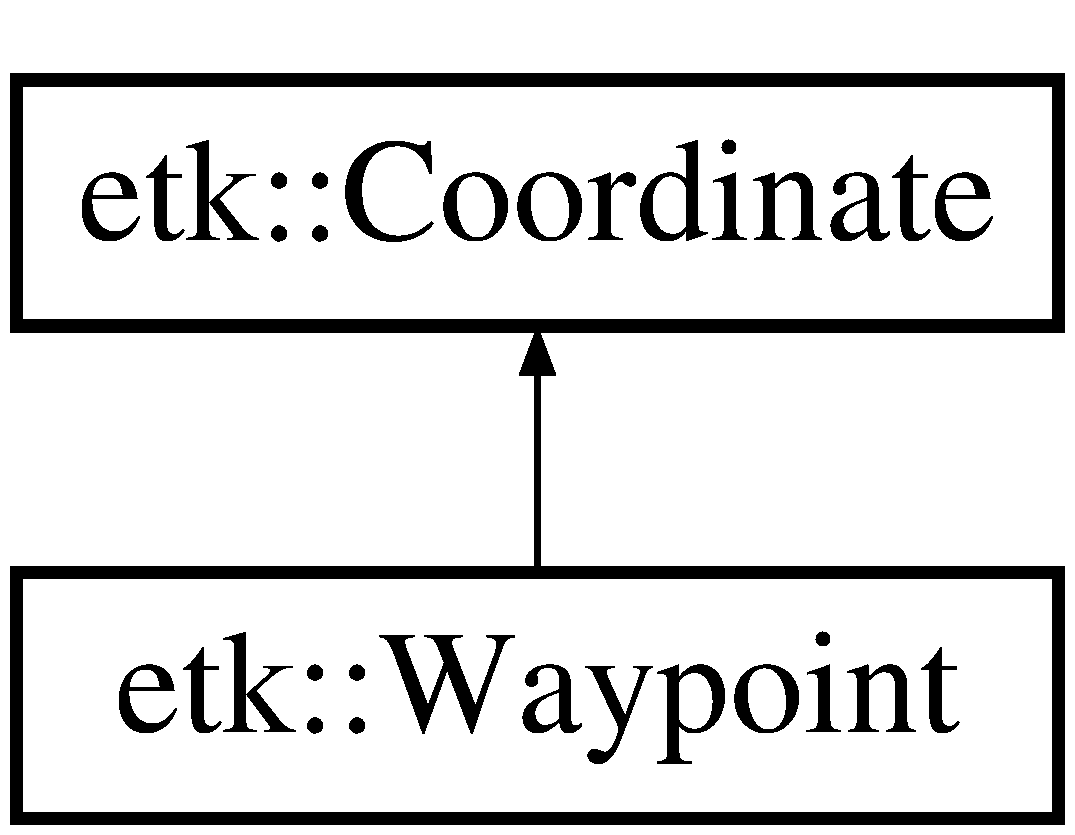
\includegraphics[height=2.000000cm]{classetk_1_1_waypoint}
\end{center}
\end{figure}
\subsection*{Public Member Functions}
\begin{DoxyCompactItemize}
\item 
\hypertarget{classetk_1_1_waypoint_a5dcd644878b98b826ddc1b56e0e3c279}{{\bfseries Waypoint} (real\-\_\-t la, real\-\_\-t ln)}\label{classetk_1_1_waypoint_a5dcd644878b98b826ddc1b56e0e3c279}

\item 
\hypertarget{classetk_1_1_waypoint_a2104309ef0f478a9f58f6b4f84e189d5}{{\bfseries Waypoint} (real\-\_\-t la, real\-\_\-t ln, real\-\_\-t a)}\label{classetk_1_1_waypoint_a2104309ef0f478a9f58f6b4f84e189d5}

\item 
\hypertarget{classetk_1_1_waypoint_a153e7a17f2de1340493b3f09f3eea3b5}{{\bfseries Waypoint} (\hyperlink{classetk_1_1_vector}{etk\-::\-Vector}$<$ 3 $>$ pos)}\label{classetk_1_1_waypoint_a153e7a17f2de1340493b3f09f3eea3b5}

\item 
\hypertarget{classetk_1_1_waypoint_a713be7c1b38ef8b77bcdf976caa69aa5}{{\bfseries operator Vector$<$ 3 $>$} ()}\label{classetk_1_1_waypoint_a713be7c1b38ef8b77bcdf976caa69aa5}

\item 
\hypertarget{classetk_1_1_waypoint_a6ab344e8ab1bbc831a0b4cf97a6eff56}{real\-\_\-t {\bfseries get\-\_\-alt} ()}\label{classetk_1_1_waypoint_a6ab344e8ab1bbc831a0b4cf97a6eff56}

\item 
\hypertarget{classetk_1_1_waypoint_ad1648e2e4c9595956ce2a773636c355b}{void {\bfseries set\-\_\-alt} (real\-\_\-t a)}\label{classetk_1_1_waypoint_ad1648e2e4c9595956ce2a773636c355b}

\end{DoxyCompactItemize}
\subsection*{Protected Attributes}
\begin{DoxyCompactItemize}
\item 
\hypertarget{classetk_1_1_waypoint_a5c301b9ba7c7f8e28f44428b04ea6edc}{real\-\_\-t {\bfseries alt} = 0}\label{classetk_1_1_waypoint_a5c301b9ba7c7f8e28f44428b04ea6edc}

\end{DoxyCompactItemize}


\subsection{Detailed Description}
A \hyperlink{classetk_1_1_waypoint}{Waypoint} I\-S\-\_\-\-A coordinate, but it has an extra dimension to store altitude. It provides get and set methods for altitude, and it can be cast to a 3 dimensional \hyperlink{classetk_1_1_vector}{etk\-::\-Vector}. 

The documentation for this class was generated from the following file\-:\begin{DoxyCompactItemize}
\item 
inc/etk/navigation.\-h\end{DoxyCompactItemize}

%--- End generated contents ---

% Index
\newpage
\phantomsection
\addcontentsline{toc}{chapter}{Index}
\printindex

\end{document}
